\documentclass[Xcolor=svgnames,mathserif]{beamer}
\usepackage[utf8]{inputenc}
\usepackage[T1]{fontenc}

\usepackage[english]{babel}
% pour les images
\usepackage{graphicx}
% pour les espaces entre les lignes : 1, 1.5, 2
\usepackage{setspace}
% pour les marges
\usepackage{geometry}
%infos générales du document
\usepackage{amsmath,amsfonts}
% pour les couleurs
\usepackage{color}
% pour mettre des url
\usepackage{url}
% pour les schémas
\usepackage[all]{xy}
% for bold symbols in mathmode
\usepackage{bm}
% biblio exotique
\usepackage{natbib}

\usetheme{metropolis}

% Customisation of the metropolis theme
\definecolor{deeppurple}{HTML}{29293D}
\definecolor{lightpurple}{HTML}{B3B3CC}
\definecolor{medpurple}{HTML}{666699}

\definecolor{deepblue}{HTML}{19194D}
\definecolor{medblue}{HTML}{333399}
\definecolor{lightblue}{HTML}{B3B3E6}


\definecolor{mygreen}{HTML}{3E750A}
\definecolor{mypink}{HTML}{B30047}
%% \definecolor{mypink}{HTML}{CC0052}

\setbeamercolor{normal text}{fg=deeppurple}
\setbeamercolor{frametitle}{bg=deeppurple}
\setbeamercolor{example text}{fg=mypink}
\setbeamercolor{accent text}{fg=myblue}
\setbeamercolor{alerted text}{fg=mypink}
\setbeamercolor{progress bar}{fg=mypink}

\metroset{sectionpage=progressbar, subsectionpage=none, progressbar=frametitle}

\newcommand{\R}{\mathbb{R}}
\newcommand{\beq}{\begin{equation}}
\newcommand{\eeq}{\end{equation}}
\newcommand{\m}[1]{\mathbf{#1}}

\newcommand{\Rcmd}[1]{
%	\begin{columns}[c]
%		\column{0.2\textwidth}
%		\column{0.5cm}
%		\includegraphics[width=.5cm]{figs/Rinvit.png}
%		\column{0.8\textwidth}
%		\alert{\scriptsize \texttt{#1}}
%	\end{columns}
}

\newcommand{\Rlogo}{
		\includegraphics[width=.5cm]{figs/Rlogo-transp.png}
}



\definecolor{gris}{gray}{0.45}

\title[~]{Introduction to phylogenetics}
\author[~]{\textbf{Thibaut Jombart}}

\institute{MRC Centre for Outbreak Analysis and Modelling\\ Imperial College London}

\date[15 December 2017]{15 December 2017}


%% Pour rappeler le plan a chaque changement de subsection.
\AtBeginSection[]
{
 \begin{frame}<beamer>
   \frametitle{Plan}
   % \tableofcontents[currentsection,currentsubsection]
   \tableofcontents[currentsection]
 \end{frame}
}

% \AtBeginSubsection[]
% {
%  \begin{frame}<beamer>
%    \frametitle{Plan}
%    % \tableofcontents[currentsection,currentsubsection]
%    \tableofcontents[currentsubsection]
%  \end{frame}
% }


%% % Pour rappeler le plan a chaque changement de subsection.
%% \AtBeginSubsection[]
%% {
%%    \begin{frame}
%%        \frametitle{Outline}
%%        \tableofcontents[currentsection,currentsubsection]
%%    \end{frame}
%% }



% Pour rappeler le plan a chaque changement de section.
\AtBeginSection[]
{
  \begin{frame}<beamer>
    \frametitle{Outline}
    \tableofcontents[currentsection]
  \end{frame}
}
%
%\AtBeginSubsection[]
%{
%  \begin{frame}<beamer>
%    \frametitle{Outline}
%    \tableofcontents[currentsubsection]
%  \end{frame}
%}

\usefonttheme[onlymath]{serif}


%% %%%%%%%%%%%%%%%%%%%%%%%%%%

\begin{document}


%%%%%%%%%%%%%%%%%%%%
%%%%%%%%%%%%%%%%%%%%
\maketitle



%%%%%%%%%%%%%%%%%%%%%%%%%%%%
%%%%%%%%%%%%%%%%%%%%%%%%%%%%
\begin{frame}[fragile]
  \frametitle{Outline}
\tableofcontents
\end{frame}




%%%%%%%%%%%%%%%%%%%%
%%%%%%%%%%%%%%%%%%%%
% pas de sections
%%%%%%%%%%%%%%%%%%%%
%%%%%%%%%%%%%%%%%%%%


%% %%%%%%%%%%%%%%%%%%%%
%% %%%%%%%%%%%%%%%%%%%%
%% \section{Context}
\subsection{~}
%% %%%%%%%%%%%%%%%%%%%%
%% %%%%%%%%%%%%%%%%%%%%

%%%%%%%%%%%%%%%%%%%%
%%%%%%%%%%%%%%%%%%%%
\begin{frame}
  \frametitle{Phylogenetics: from the origins...}

\begin{columns}[l]
	\column{.5\textwidth}
	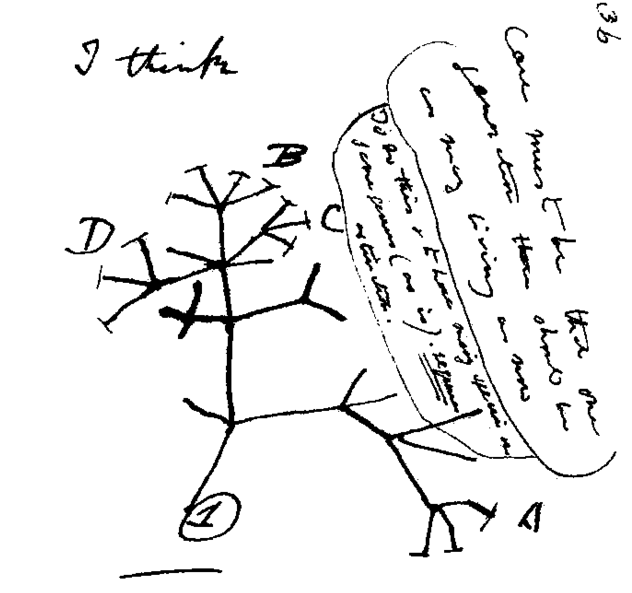
\includegraphics[width=\textwidth]{figs/DarwinTree.png}\\
	C. Darwin, Notebook, 1837.	
	\column{0.6\textwidth}
	\textit{'From the first growth of the tree, many a limb and branch has decayed and dropped off; and these fallen branches of various sizes may represent those whole orders, families, and genera which have now no living representatives, and which are known to us only in a fossil state.'}
\end{columns}

\end{frame}

%%%%%%%%%%%%%%%%%%%%
%%%%%%%%%%%%%%%%%%%%






%%%%%%%%%%%%%%%%%%%%
%%%%%%%%%%%%%%%%%%%%
\begin{frame}
  \frametitle{Phylogenetics: ...to the present}

\begin{columns}[c]
	\column{.5\textwidth}
	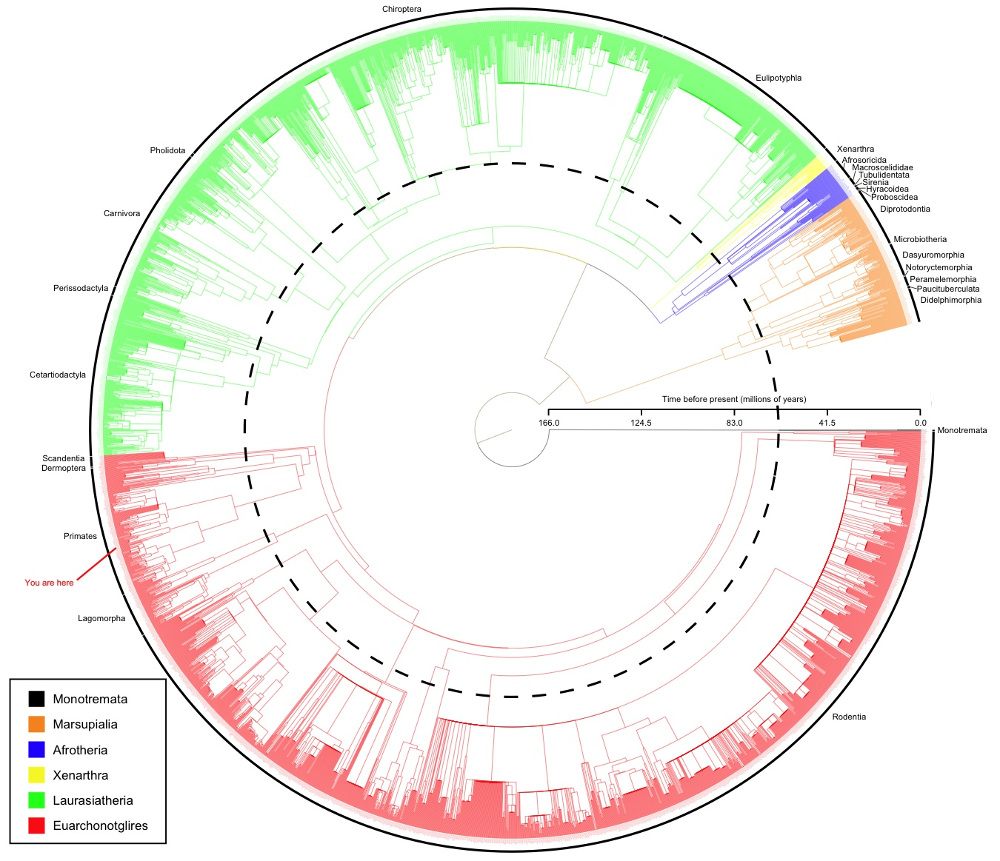
\includegraphics[width=\textwidth]{figs/mammalsTree}\\
	Bininda-Emonds \textit{et al.}, 2007, Nature.
	\column{0.6\textwidth}
\begin{itemize}
\item phylogenetic trees are part of the standard toolbox of genetic data analysis
\item represent the evolutionary history of a set of (sampled) taxa
% \item infers Most Recent Common Ancestors (MRCA)
\end{itemize}
\end{columns}


\end{frame}
%%%%%%%%%%%%%%%%%%%%
%%%%%%%%%%%%%%%%%%%%





%%%%%%%%%%%%%%%%%%%%
%%%%%%%%%%%%%%%%%%%%
\begin{frame}
  \frametitle{And the main difference is...}

\pause
\begin{columns}[c]
	\column{.5\textwidth}
	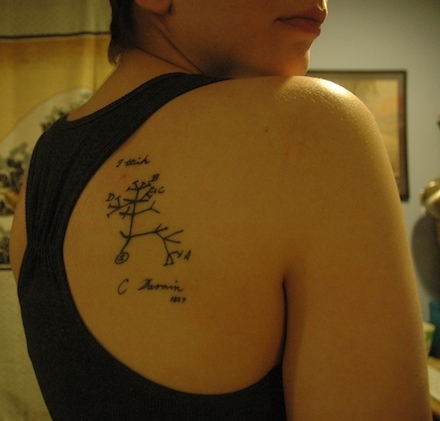
\includegraphics[width=.9\textwidth]{figs/tattooDarwin}\\
	\column{0.5\textwidth}
	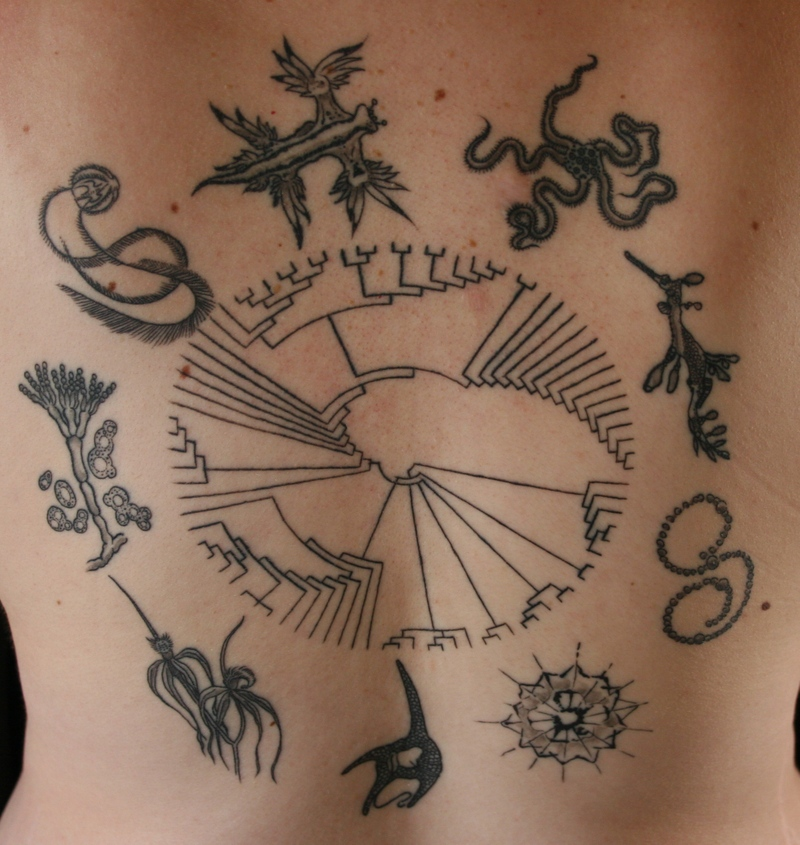
\includegraphics[width=.8\textwidth]{figs/tattooNew}\\
\end{columns}
~\\
\centering
\textbf{Current trees look better!}
\pause
~\\

\vspace{.5cm}
\alert{(and some other minor differences)}

\end{frame}
%%%%%%%%%%%%%%%%%%%%
%%%%%%%%%%%%%%%%%%%%





%%%%%%%%%%%%%%%%%%%%
%%%%%%%%%%%%%%%%%%%%
\begin{frame}
  \frametitle{About the minor differences...}

\begin{columns}[c]
	\column{.6\textwidth}
\begin{itemize}
\item DNA sequencing revolution
\item huge data banks freely available (e.g. GenBank)
\item easier, cheaper, faster to obtain DNA sequences
\item increasing number of full genomes available
\end{itemize}
	\column{0.4\textwidth}
	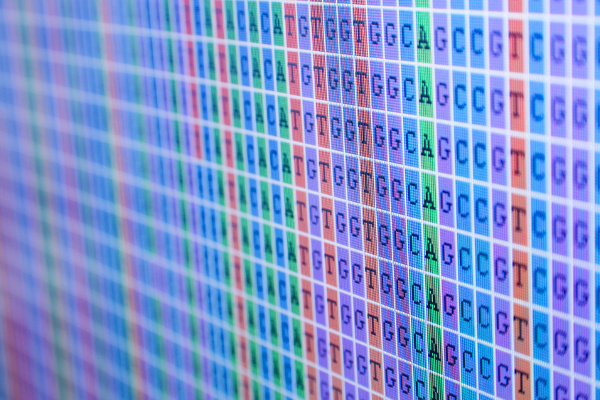
\includegraphics[width=\textwidth]{figs/DNAsequences}\\
	\end{columns}
~\\
\vspace{1cm}
\centering
\pause
\textbf{Different ways to exploit this information.}

\end{frame}
%%%%%%%%%%%%%%%%%%%%
%%%%%%%%%%%%%%%%%%%%





%%%%%%%%%%%%%%%%%%%%
%%%%%%%%%%%%%%%%%%%%
\section{Phylogenies...}
\subsection{~}
%%%%%%%%%%%%%%%%%%%%
%%%%%%%%%%%%%%%%%%%%


%
%%%%%%%%%%%%%%%%%%%%%
%%%%%%%%%%%%%%%%%%%%%
%\begin{frame}
%  \frametitle{Reconstructing evolutionary history}
%
%\vspace{.5cm}
%
%\vspace{-.5cm}
%
%\pause
%\begin{center}
%    \only<2>{\resizebox{\textwidth}{!}{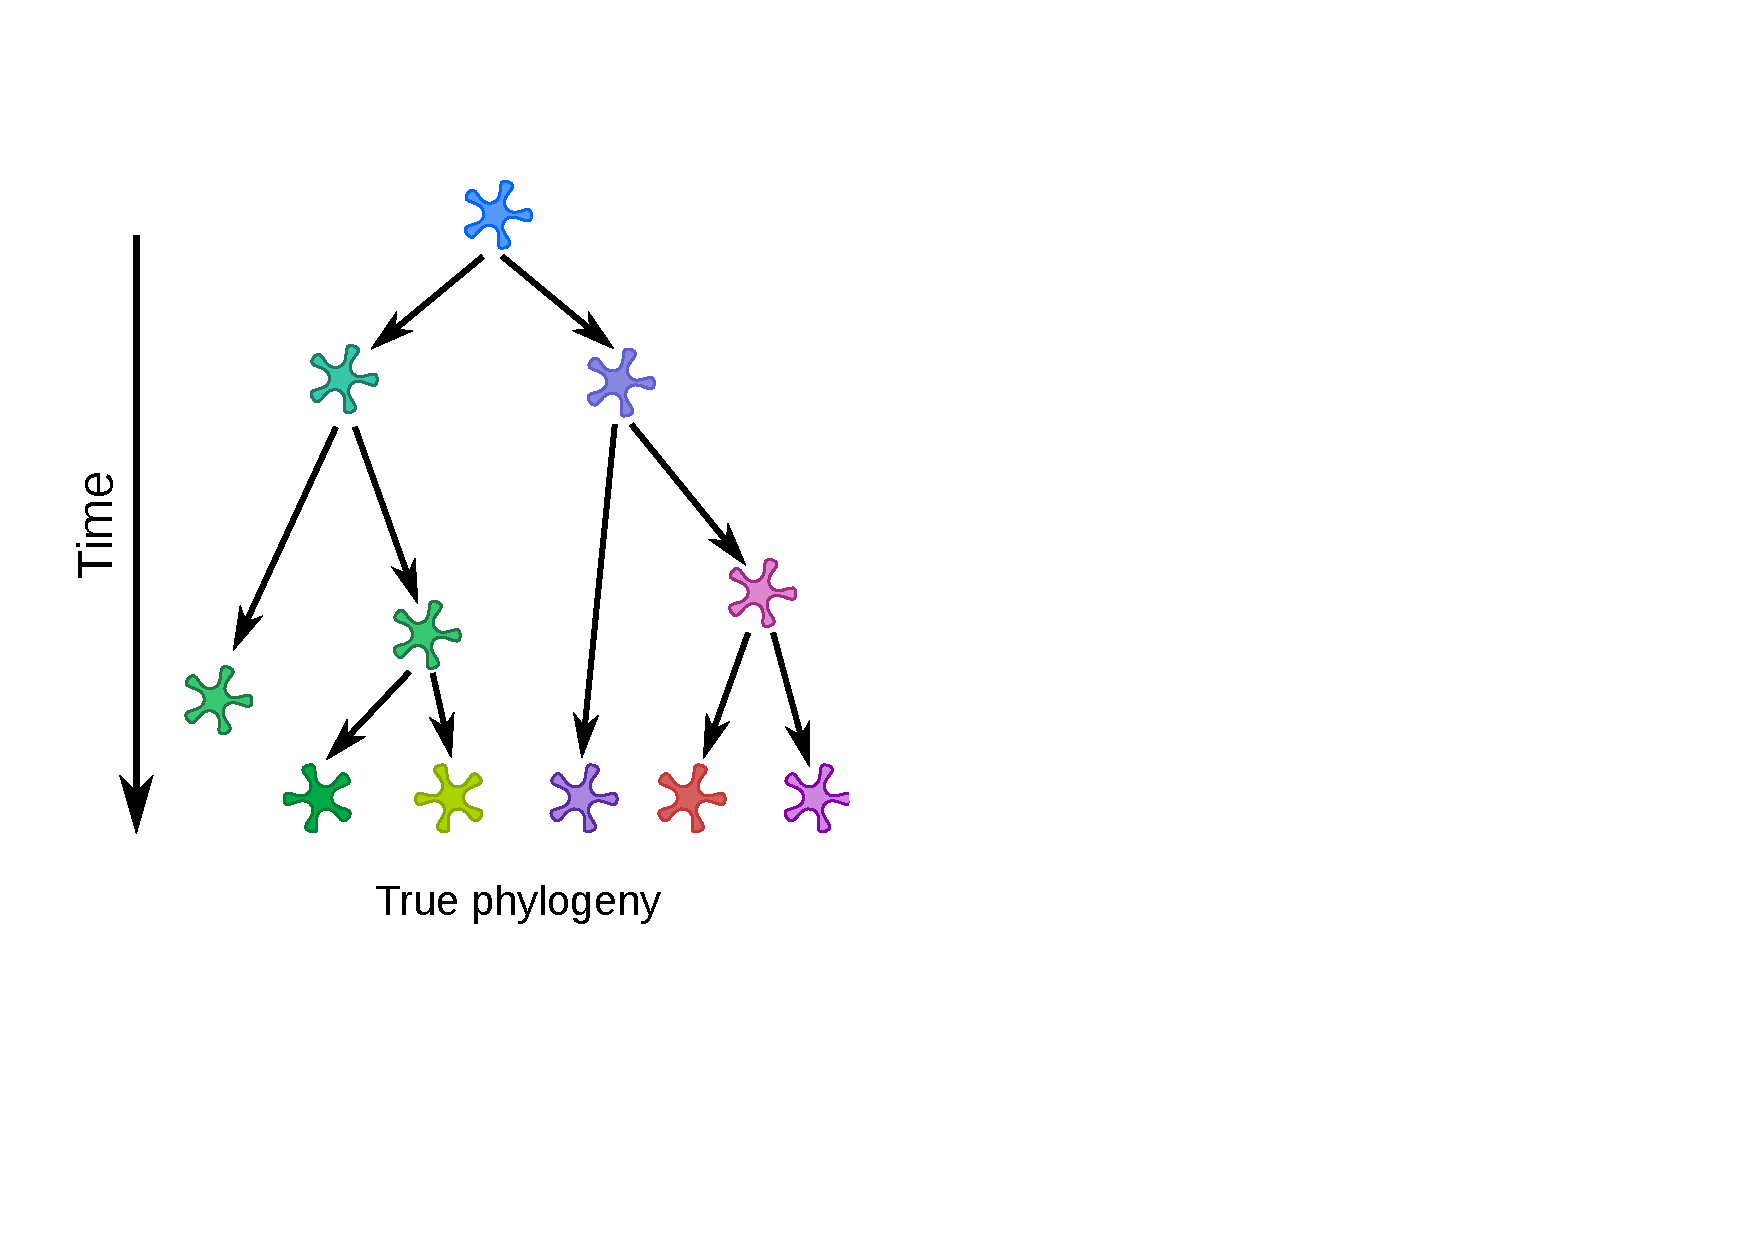
\includegraphics{figs/phylogenetics1}}}\only<3>{\resizebox{\textwidth}{!}{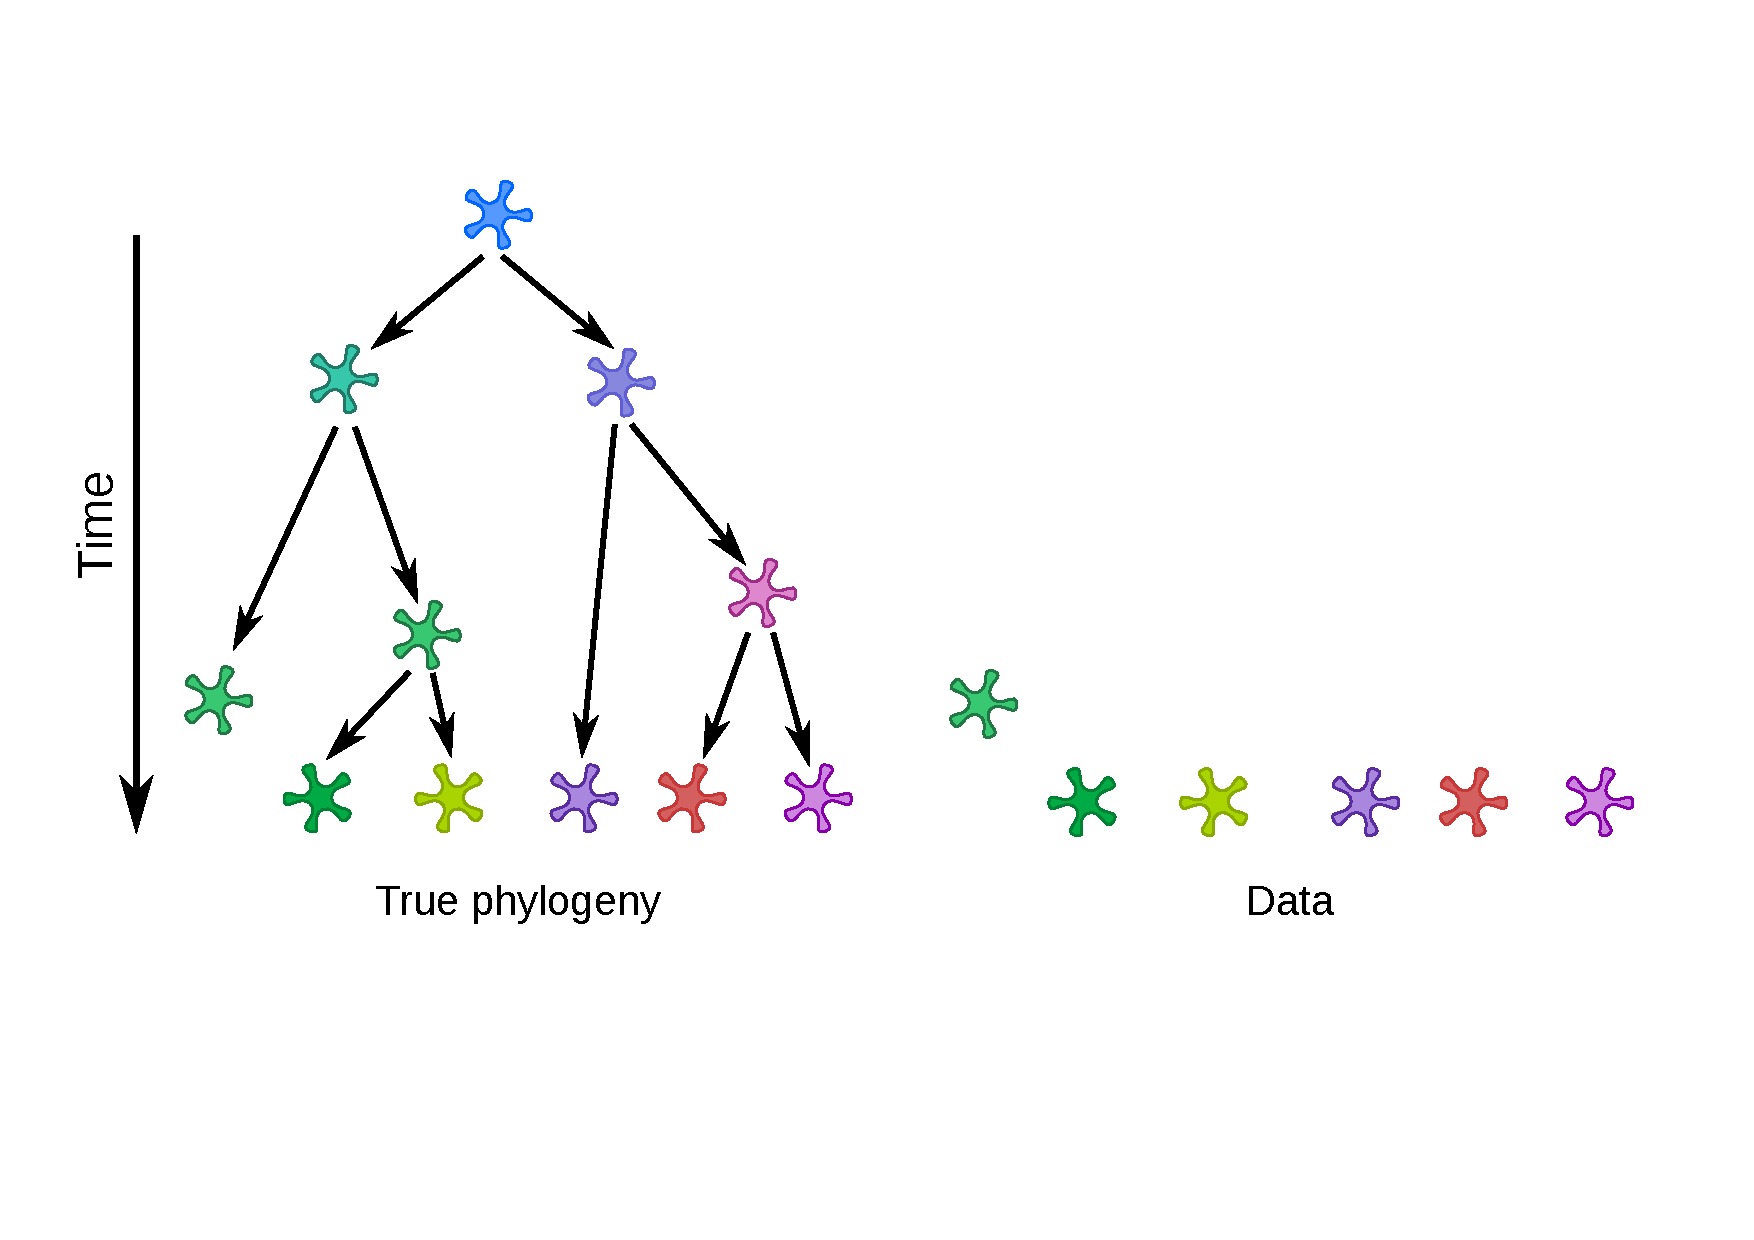
\includegraphics{figs/phylogenetics2}}}\only<4->{\resizebox{\textwidth}{!}{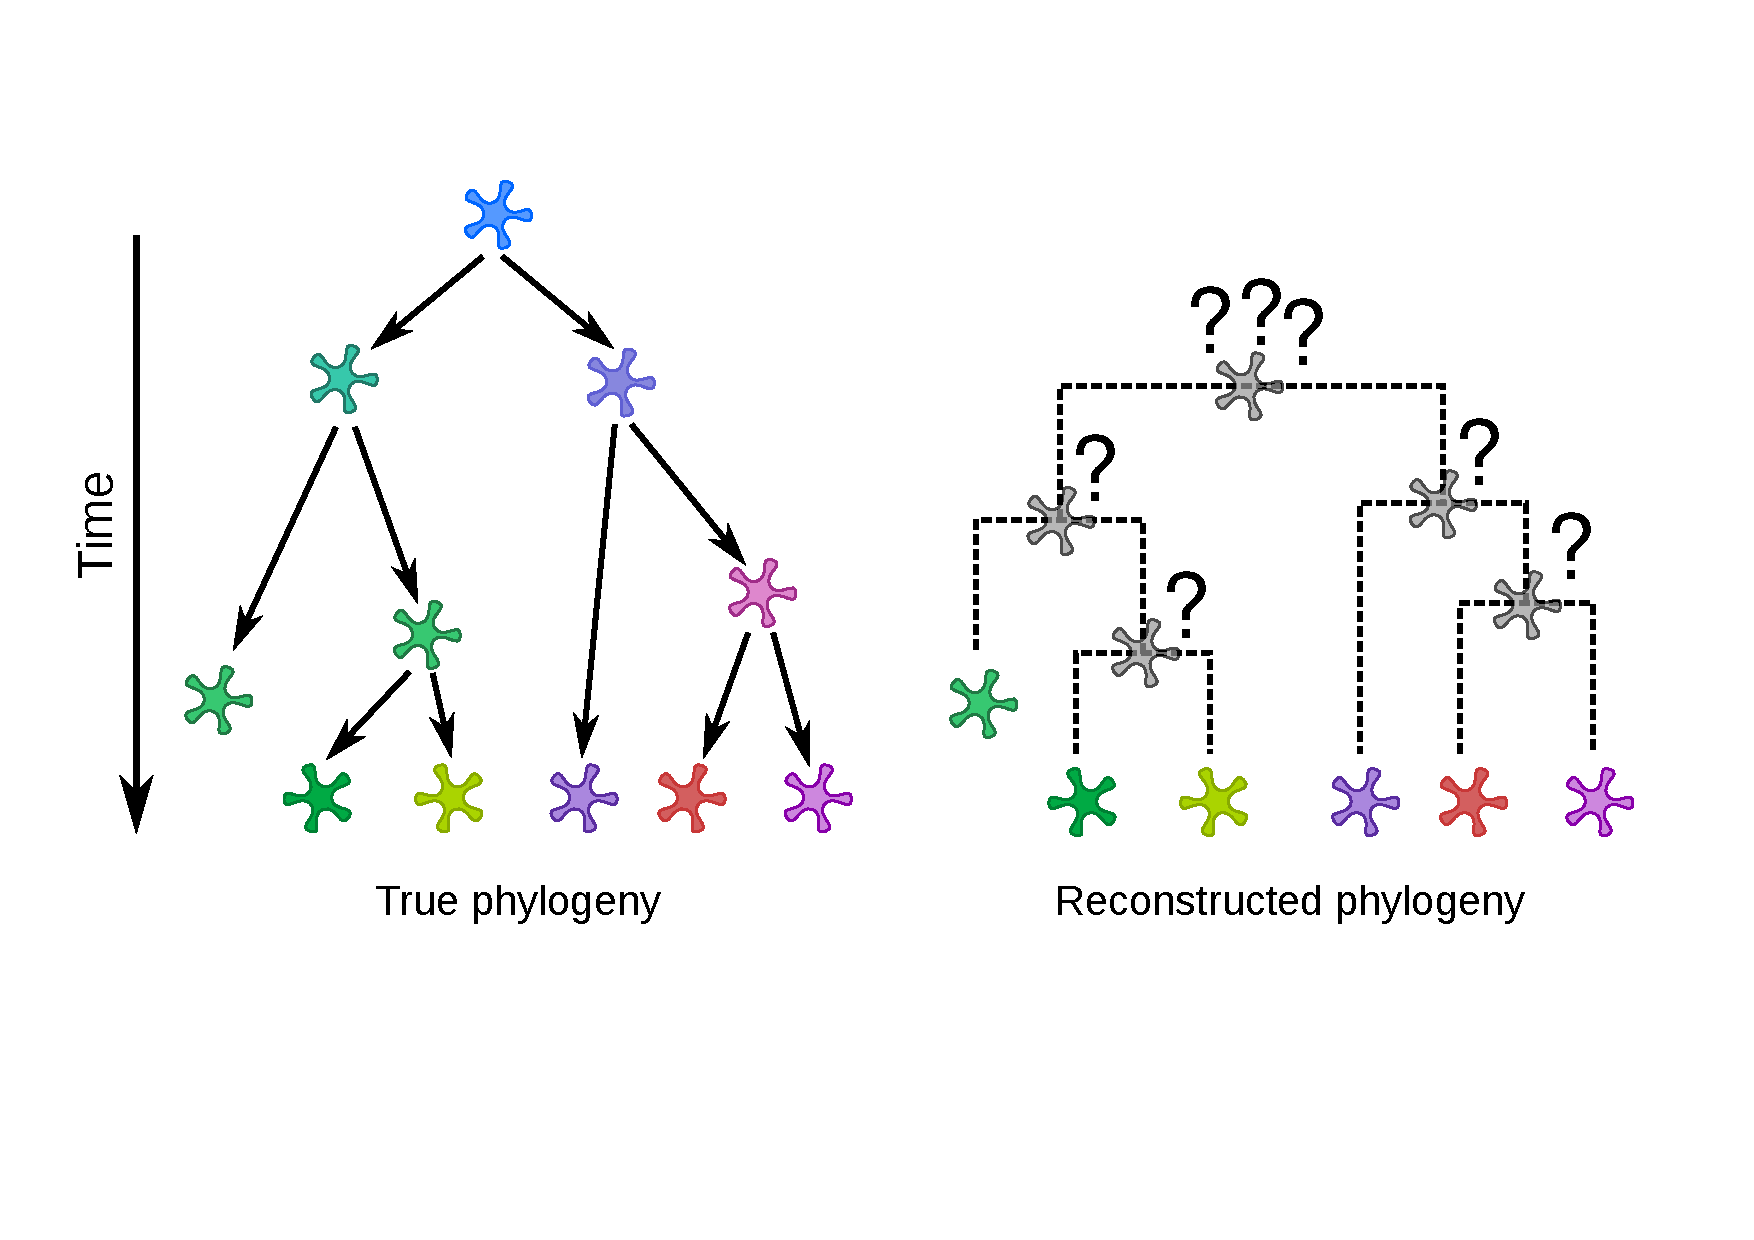
\includegraphics{figs/phylogenetics3}}}
%  \end{center}
%
%\end{frame}
%
%%%%%%%%%%%%%%%%%%%%%
%%%%%%%%%%%%%%%%%%%%%




%%%%%%%%%%%%%%%%%%%%
%%%%%%%%%%%%%%%%%%%%
\begin{frame}
  \frametitle{Genetic changes (substitution) accumulate over time}

\vspace{.5cm}
\textbf{Substitution}: replacement of a nucleotide (e.g. a $\rightarrow$ t)
\vspace{-.25cm}

\begin{center}
    \only<1>{\resizebox{.7\textwidth}{!}{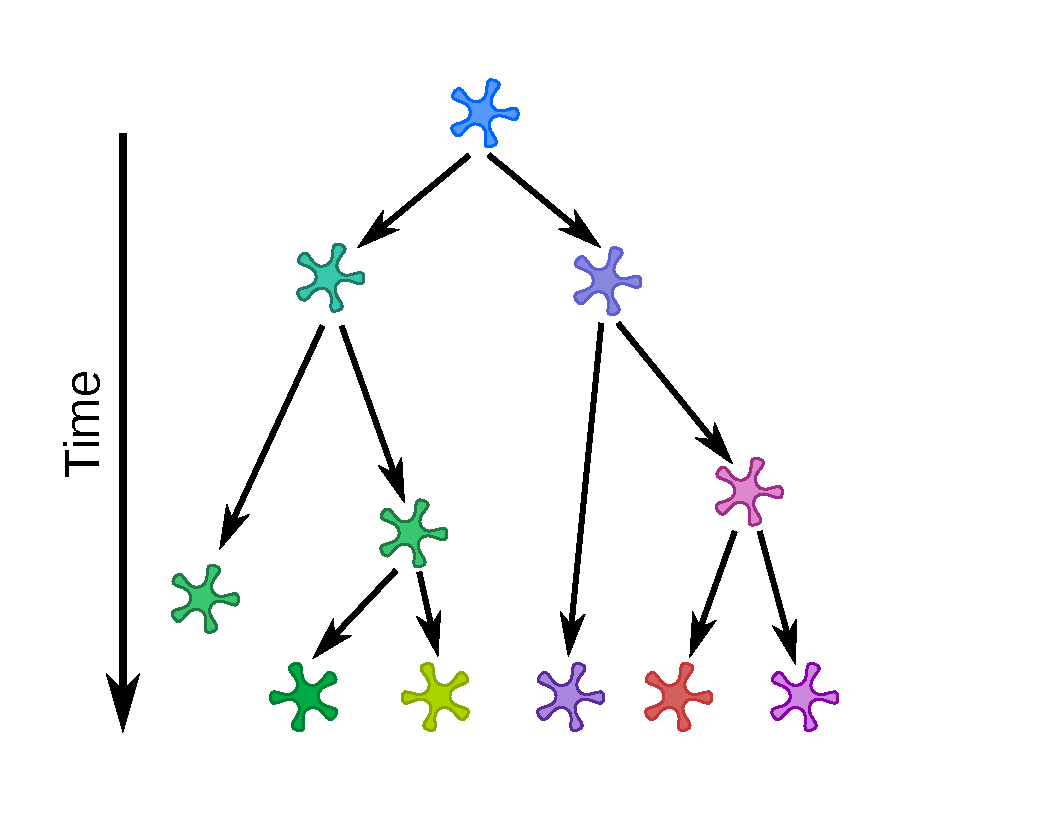
\includegraphics{figs/phyloDNA1}}}\only<2>{\resizebox{.7\textwidth}{!}{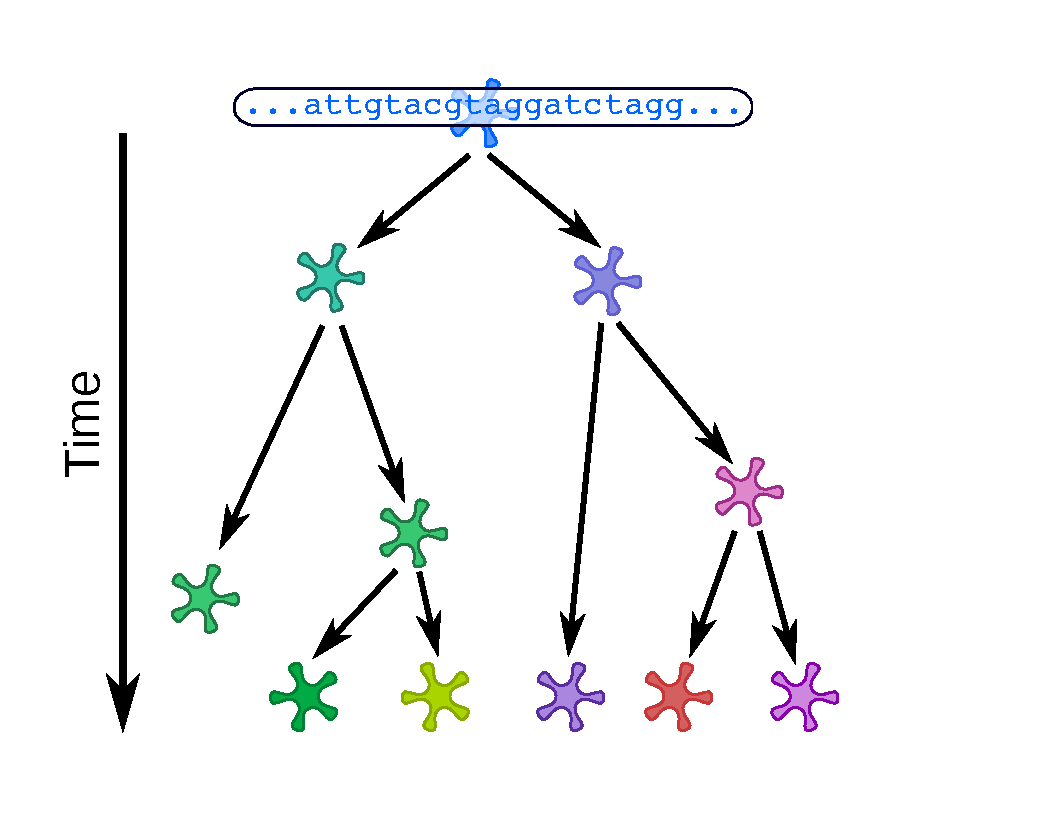
\includegraphics{figs/phyloDNA2}}}\only<3>{\resizebox{.7\textwidth}{!}{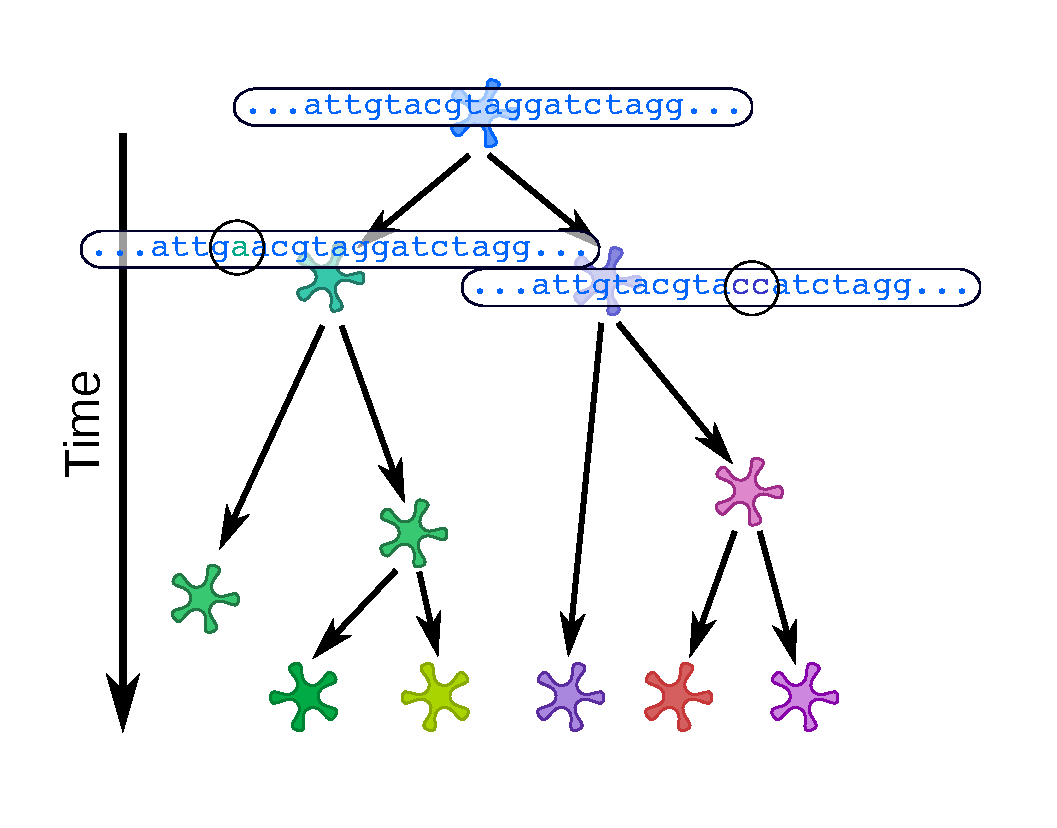
\includegraphics{figs/phyloDNA3}}}\only<4>{\resizebox{.7\textwidth}{!}{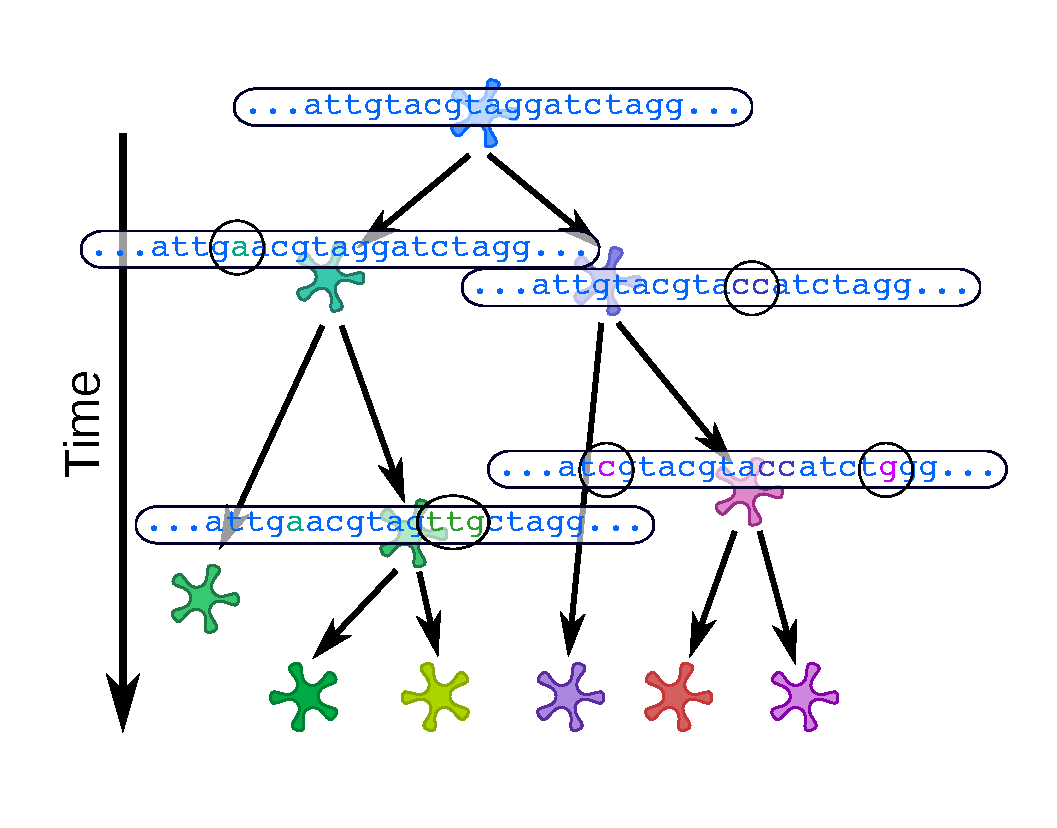
\includegraphics{figs/phyloDNA4}}}\only<5->{\resizebox{.7\textwidth}{!}{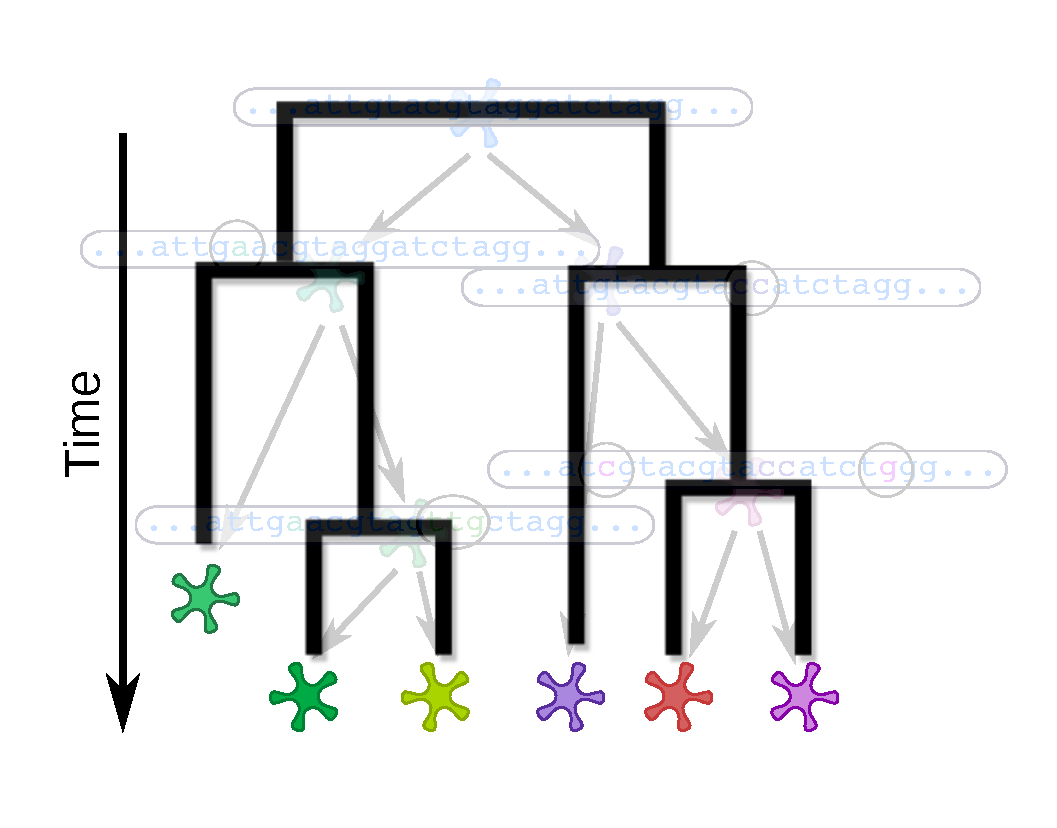
\includegraphics{figs/phyloDNA5}}}

      \visible<6->{Substitution patterns reflect the evolutionary history}

    \end{center}

\end{frame}
%%%%%%%%%%%%%%%%%%%%
%%%%%%%%%%%%%%%%%%%%




%%%%%%%%%%%%%%%%%%%%
%%%%%%%%%%%%%%%%%%%%
\begin{frame}
  \frametitle{Using substitution patterns to reconstruct the evolutionary history}

\begin{center}
    \only<1>{\resizebox{\textwidth}{!}{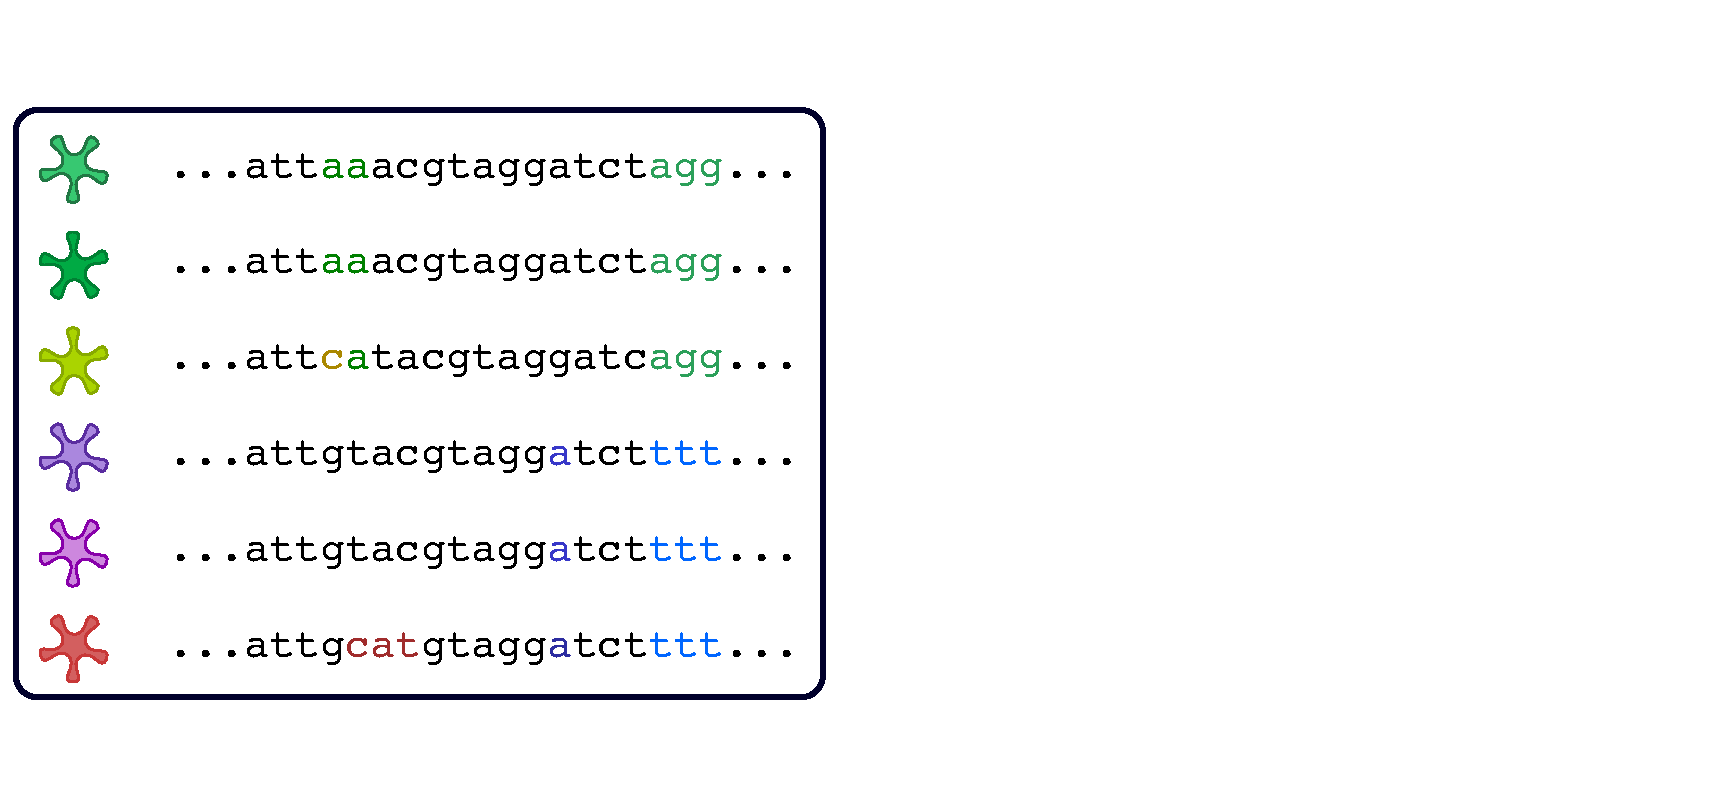
\includegraphics{figs/DNA2phylo1}}}\only<2->{\resizebox{\textwidth}{!}{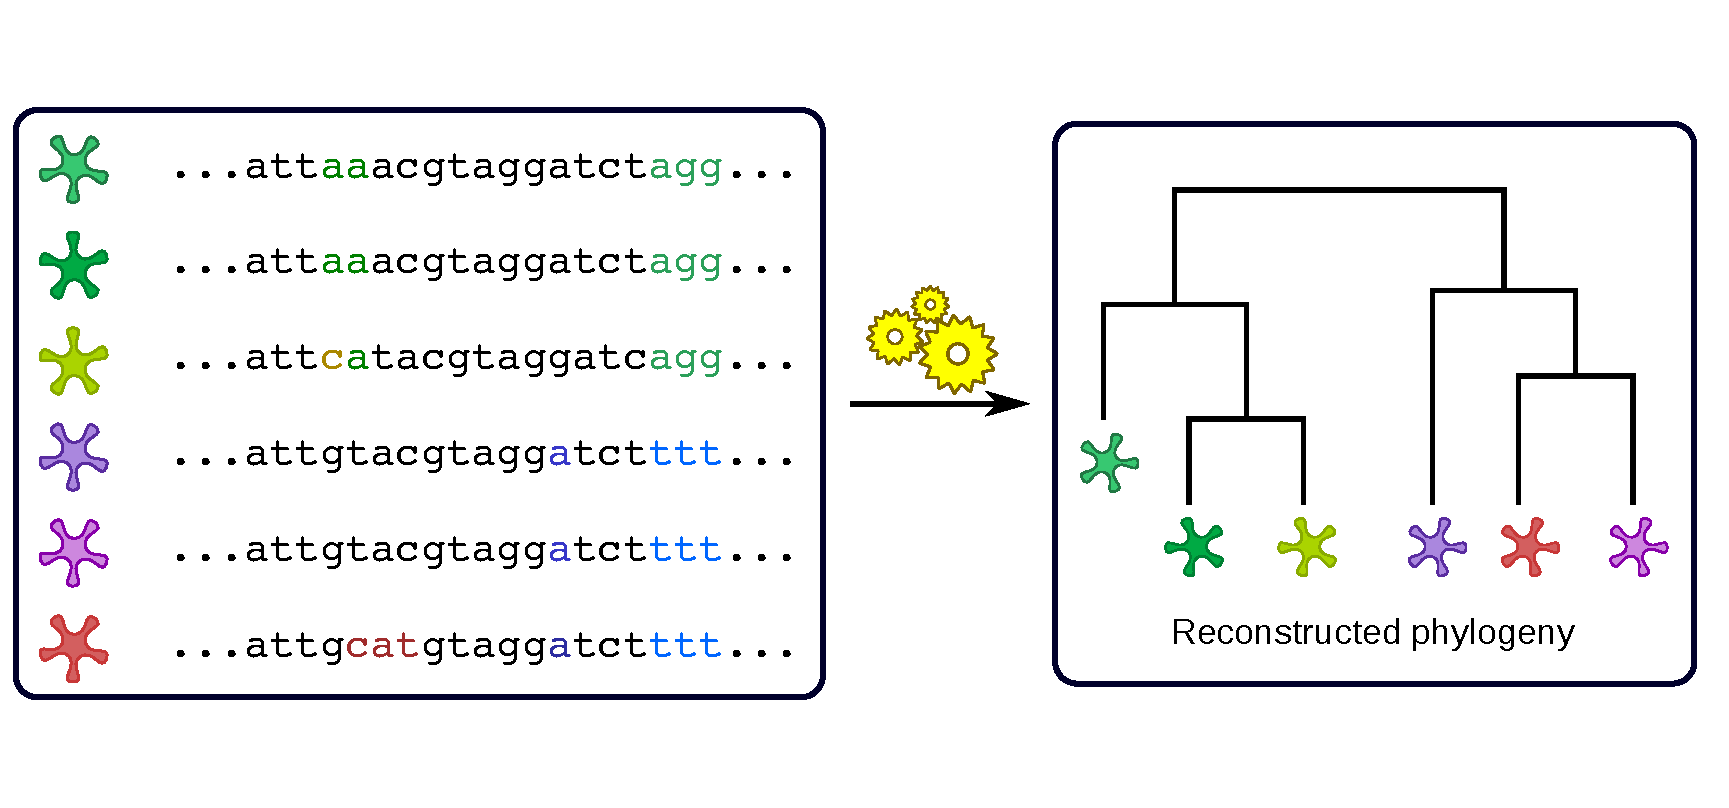
\includegraphics{figs/DNA2phylo2}}}

\visible<3->{Phylogenetics aim to reconstruct evolutionary trees (\emph{phylogenies}) from genetic sequence data.}
\end{center}

\end{frame}

%%%%%%%%%%%%%%%%%%%%
%%%%%%%%%%%%%%%%%%%%





%%%%%%%%%%%%%%%%%%%%
%%%%%%%%%%%%%%%%%%%%
\begin{frame}
  \frametitle{Using trees to represent the evolutionary history}

  \vspace{-1cm}

\begin{center}
\only<1>{\resizebox{\textwidth}{!}{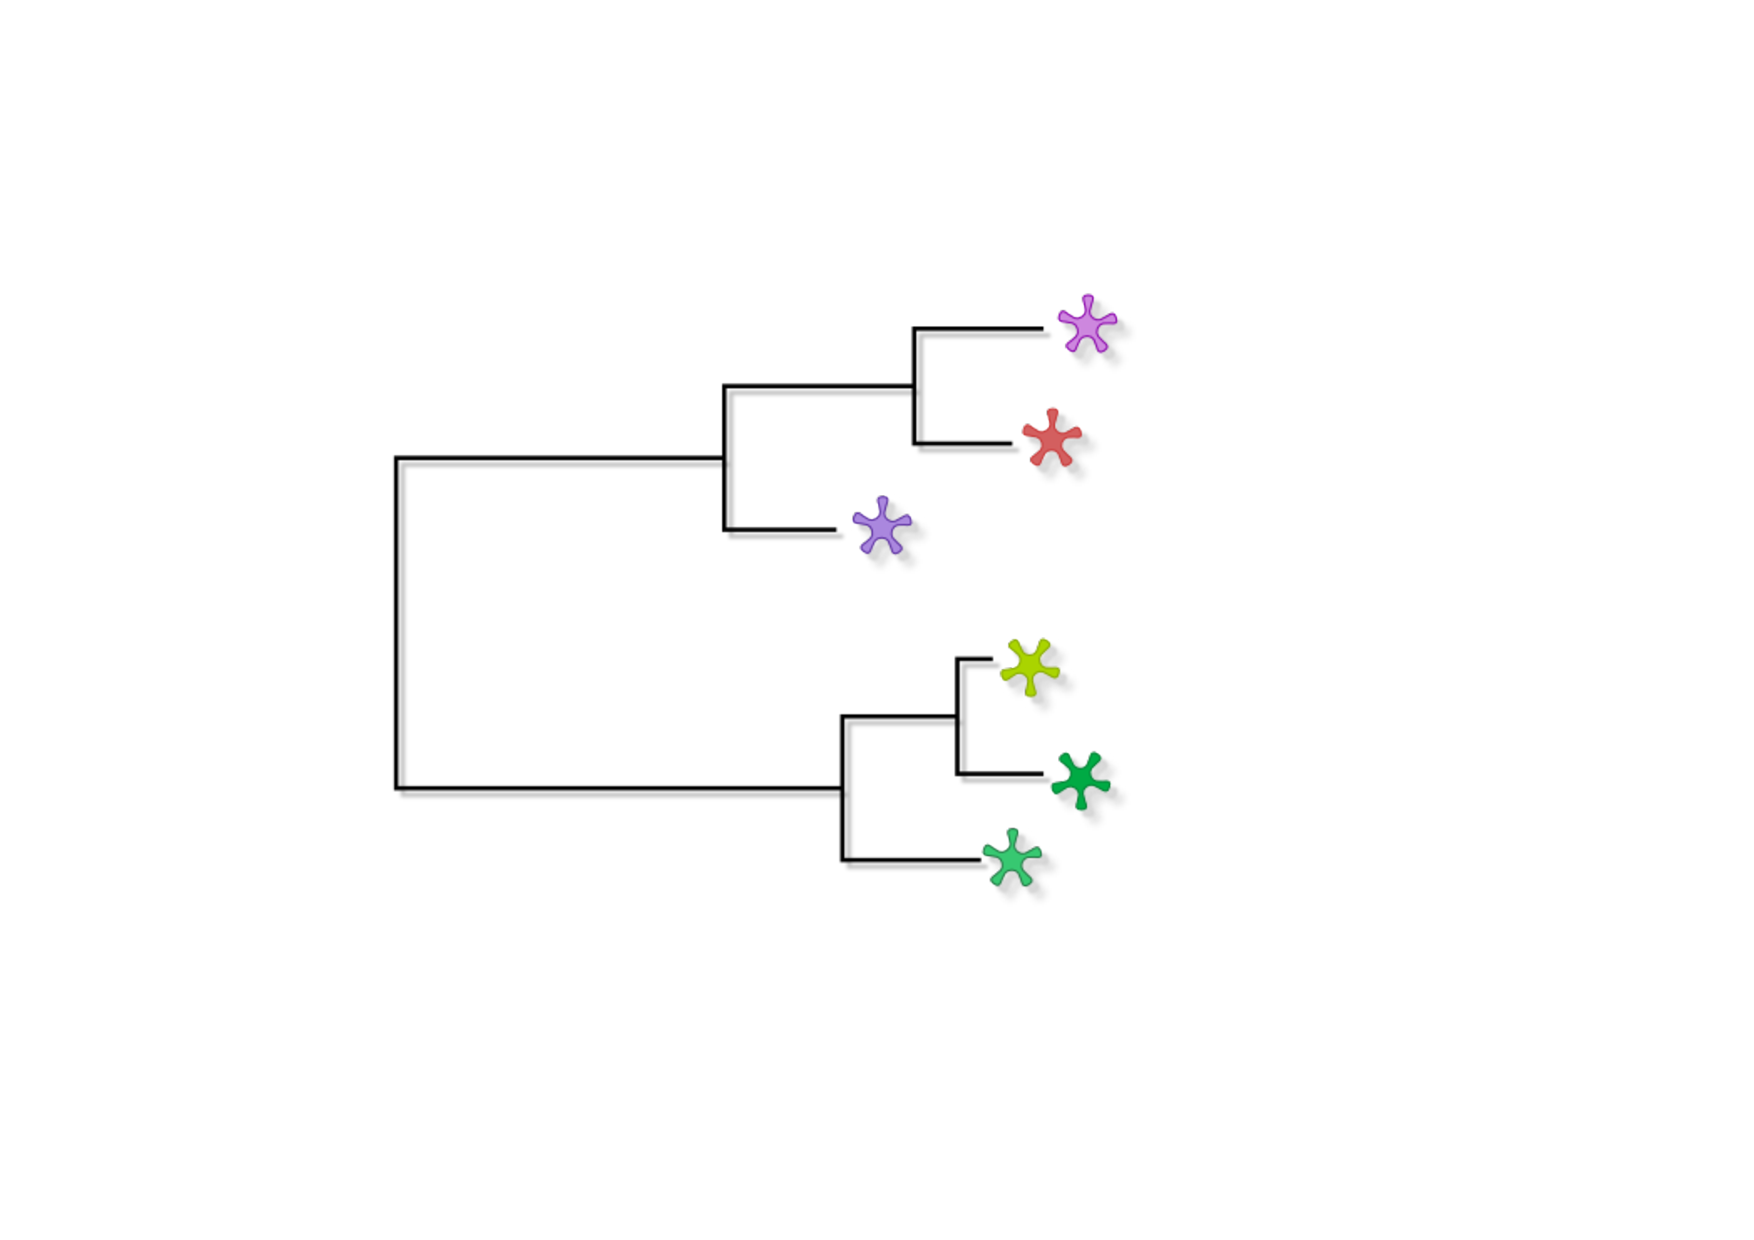
\includegraphics{figs/treeItemsEmpty}}}\only<2>{\resizebox{\textwidth}{!}{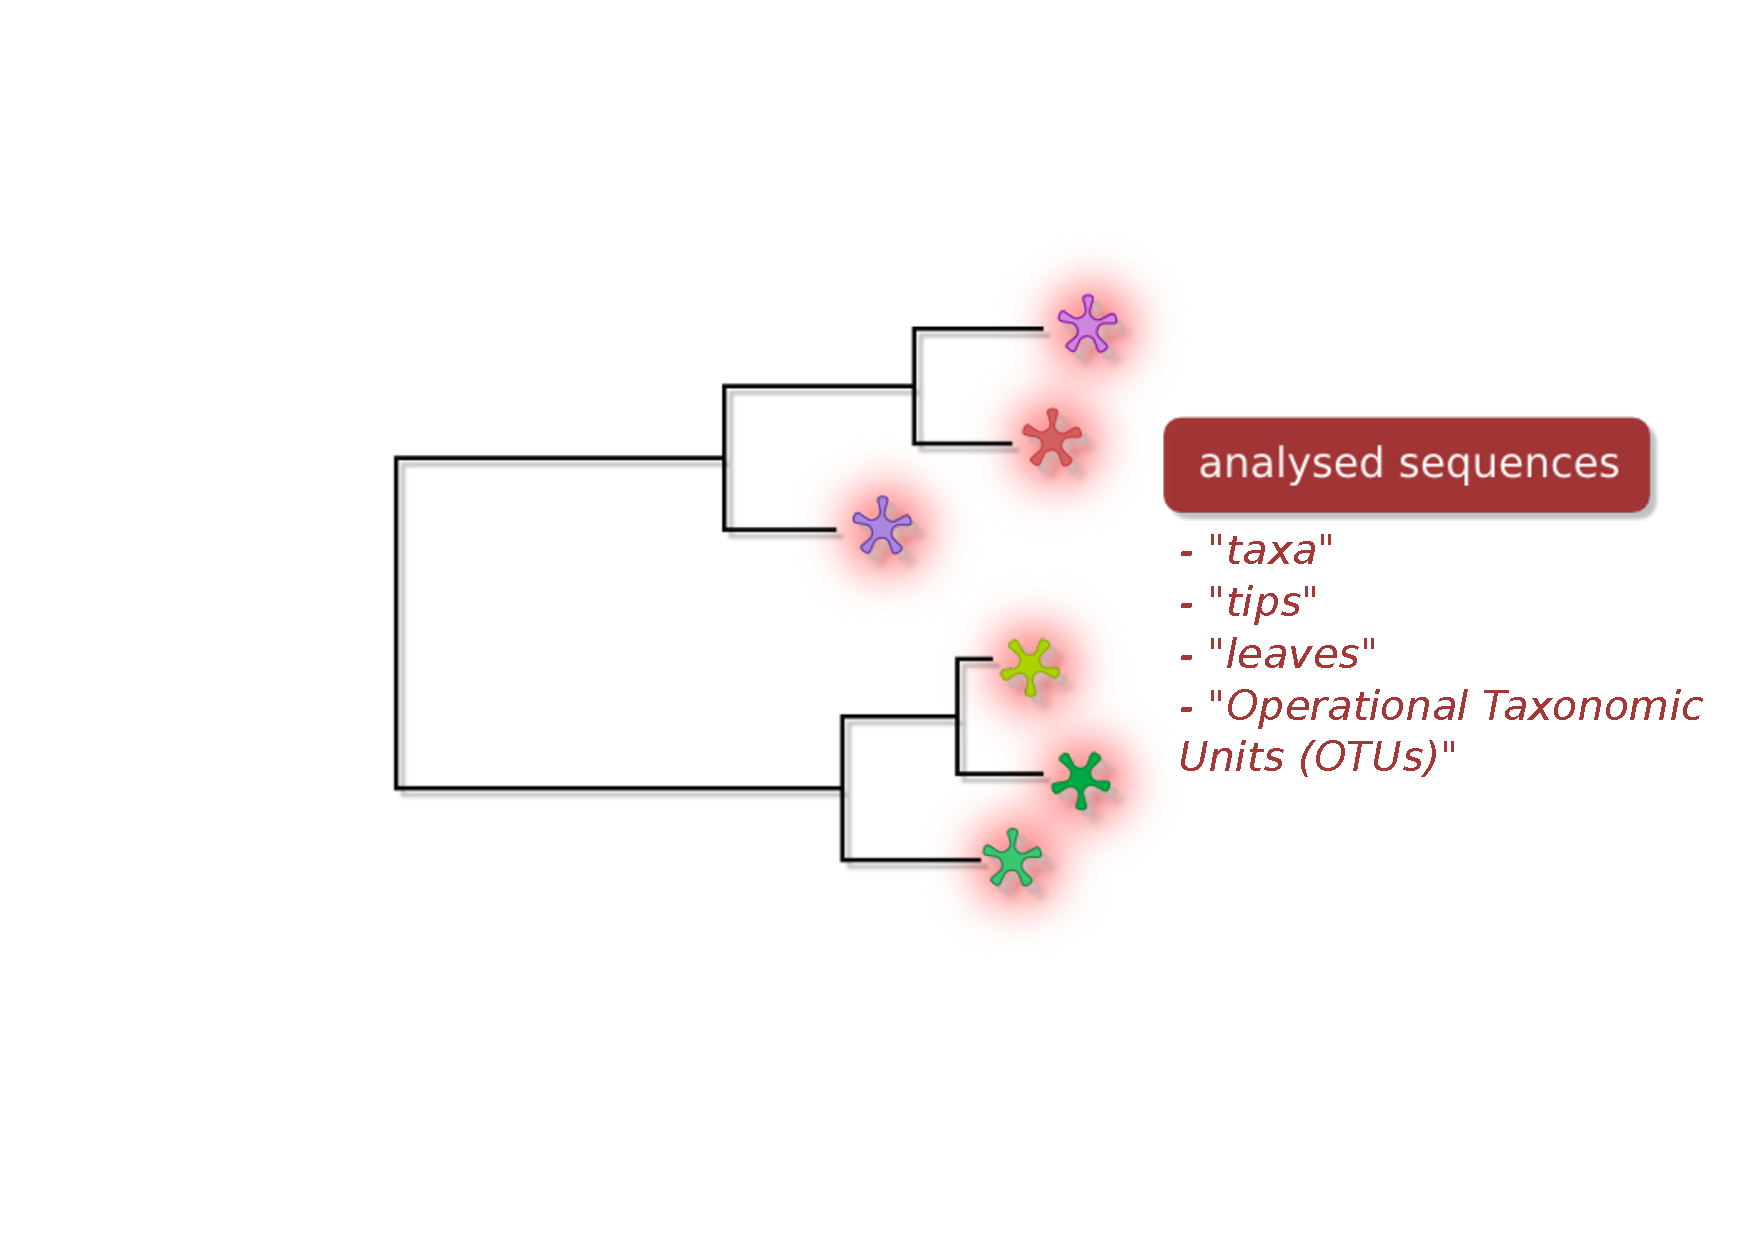
\includegraphics{figs/treeItemsTips}}}\only<3>{\resizebox{\textwidth}{!}{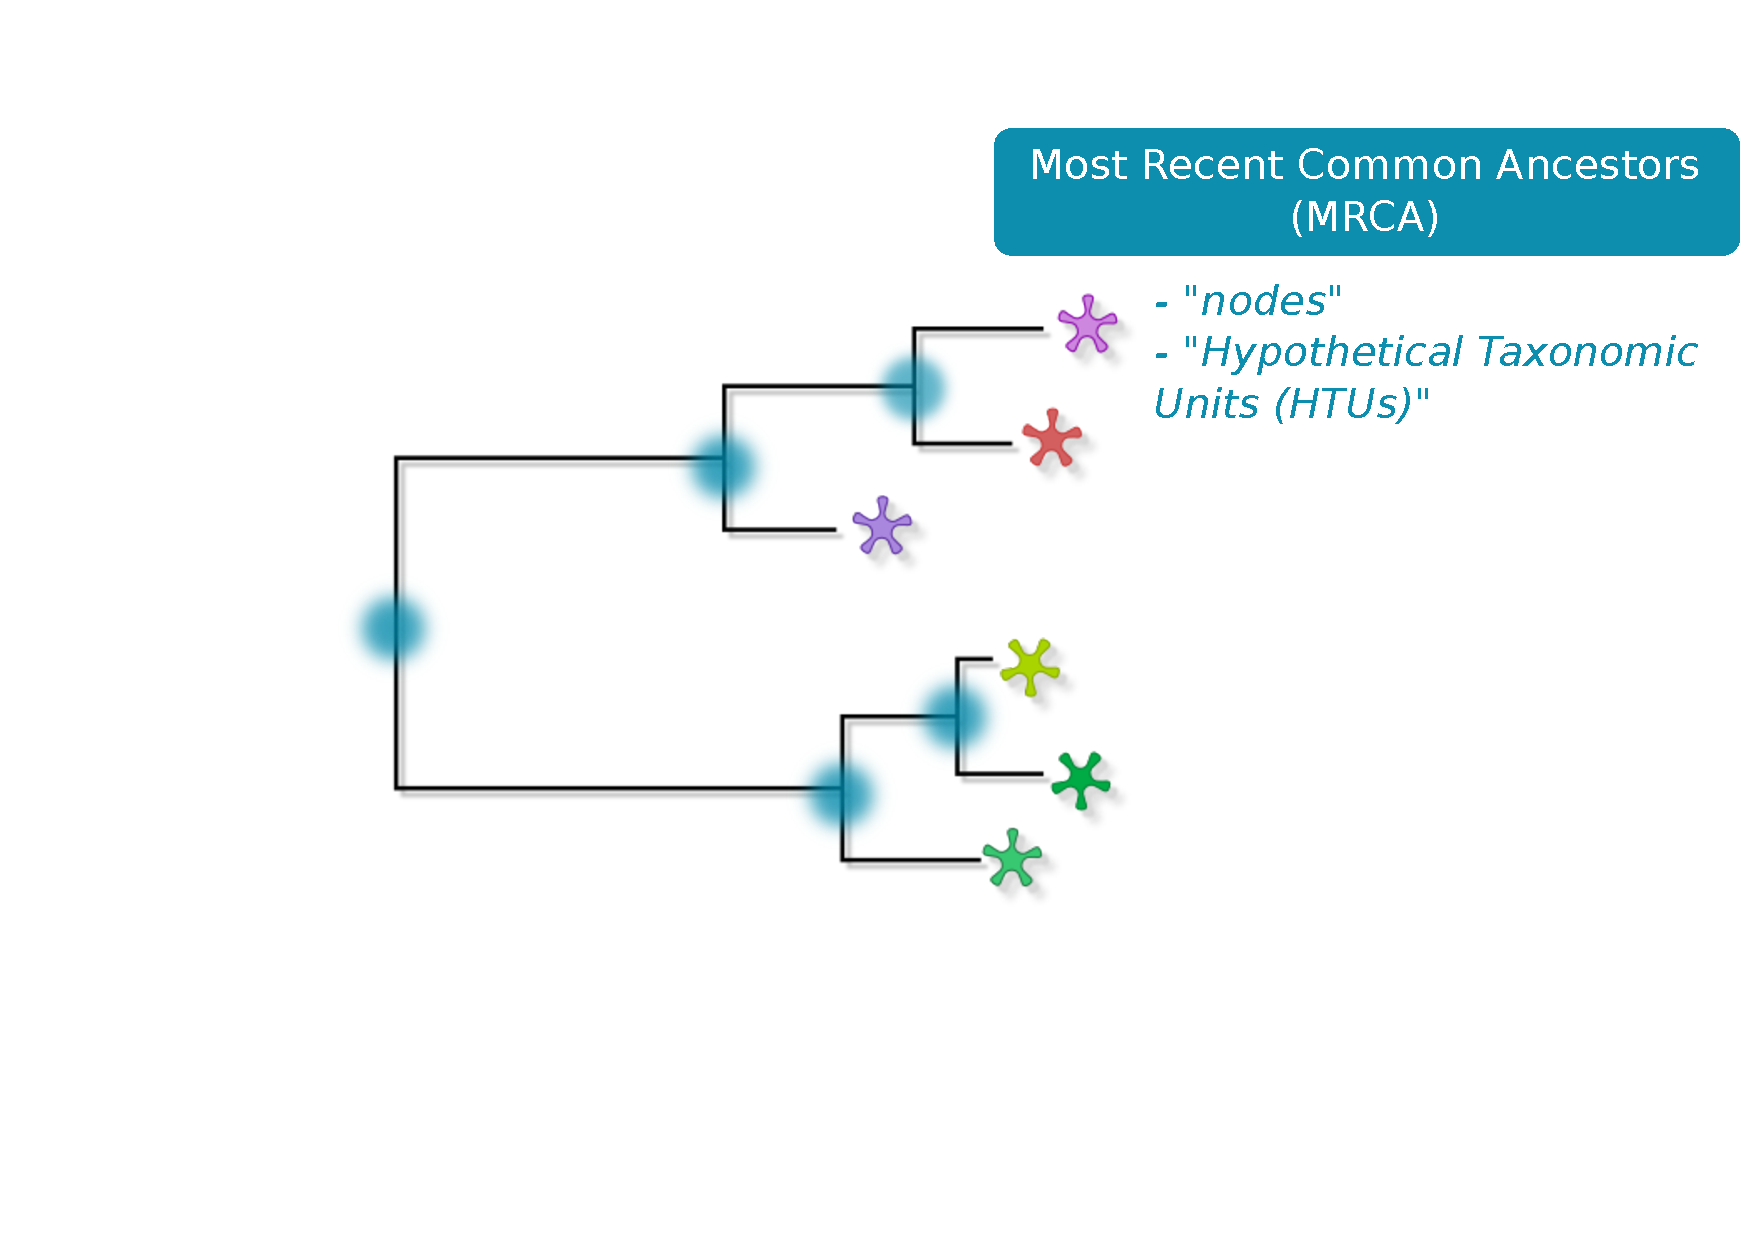
\includegraphics{figs/treeItemsNodes}}}\only<4>{\resizebox{\textwidth}{!}{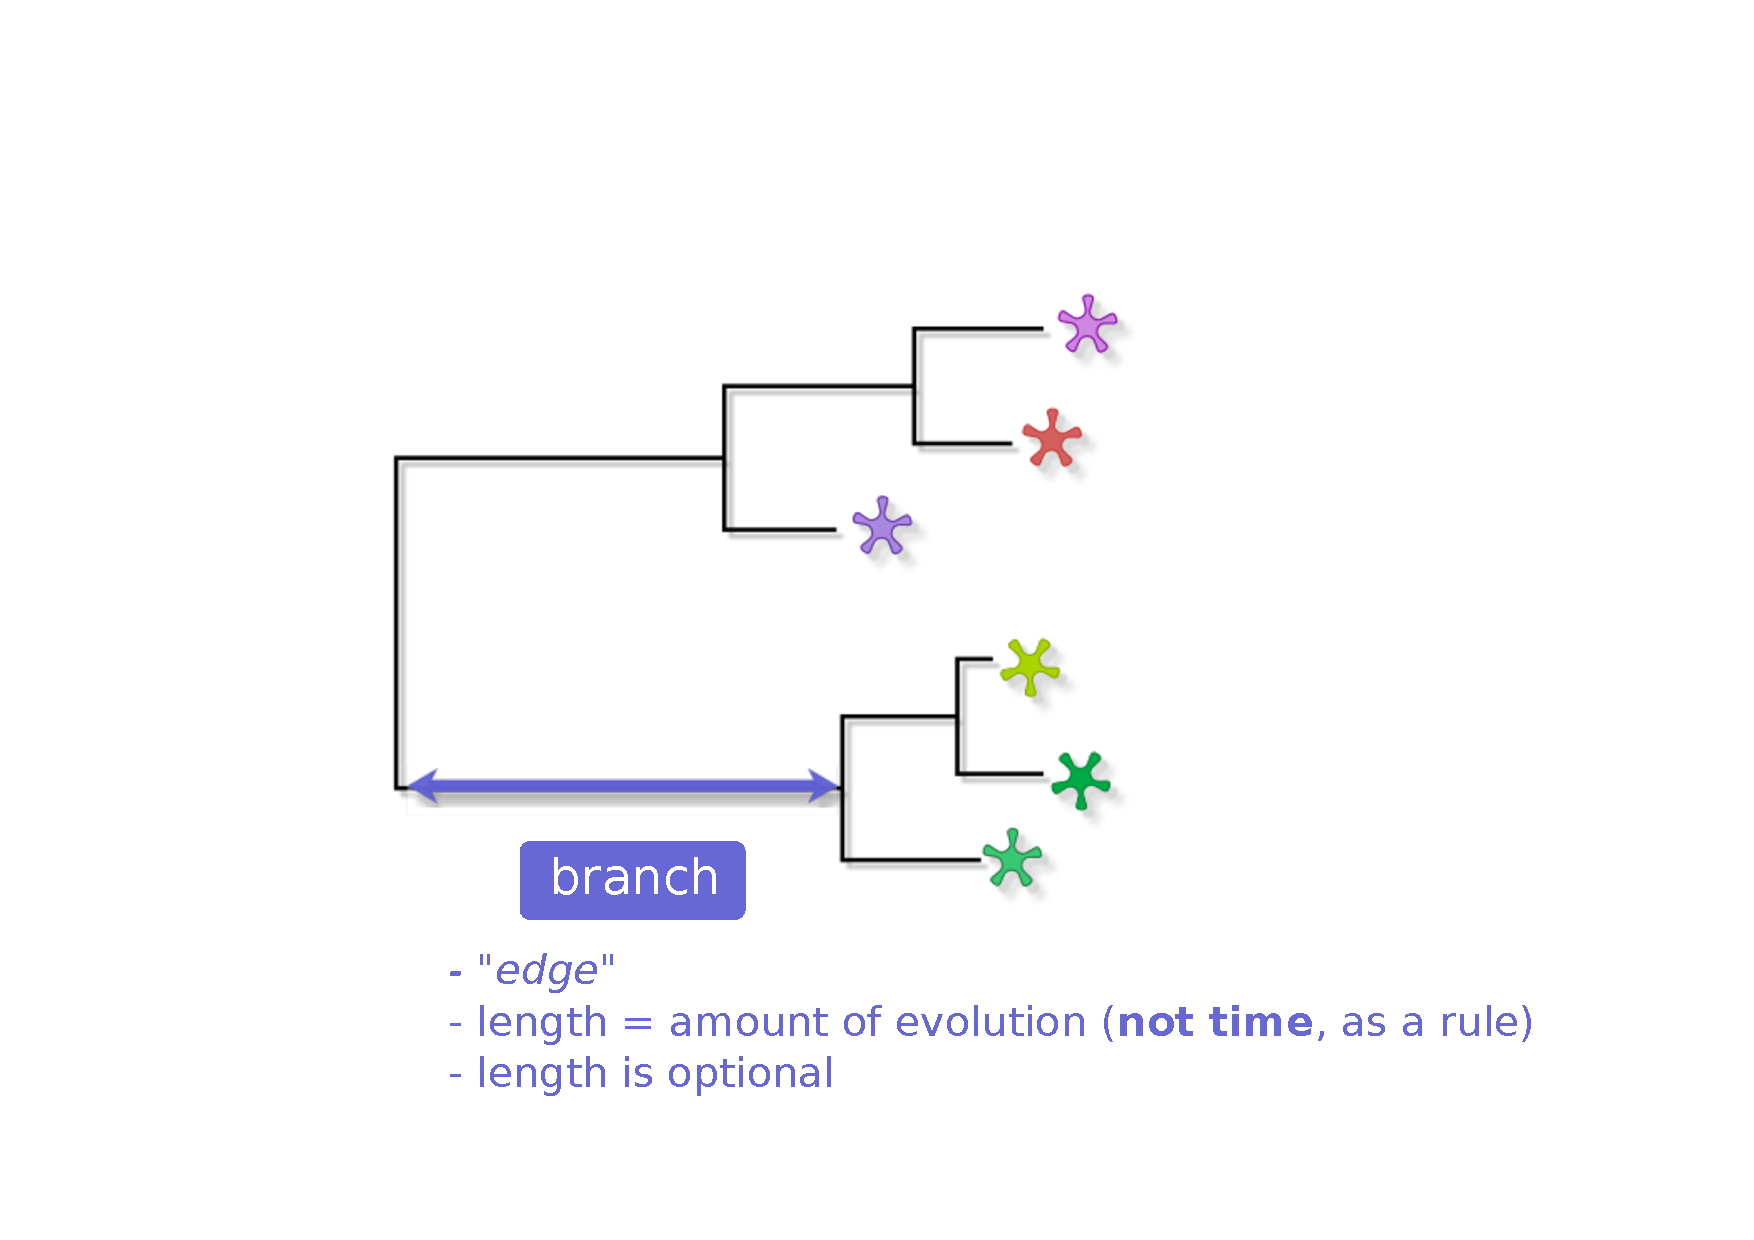
\includegraphics{figs/treeItemsBranch}}}\only<5>{\resizebox{\textwidth}{!}{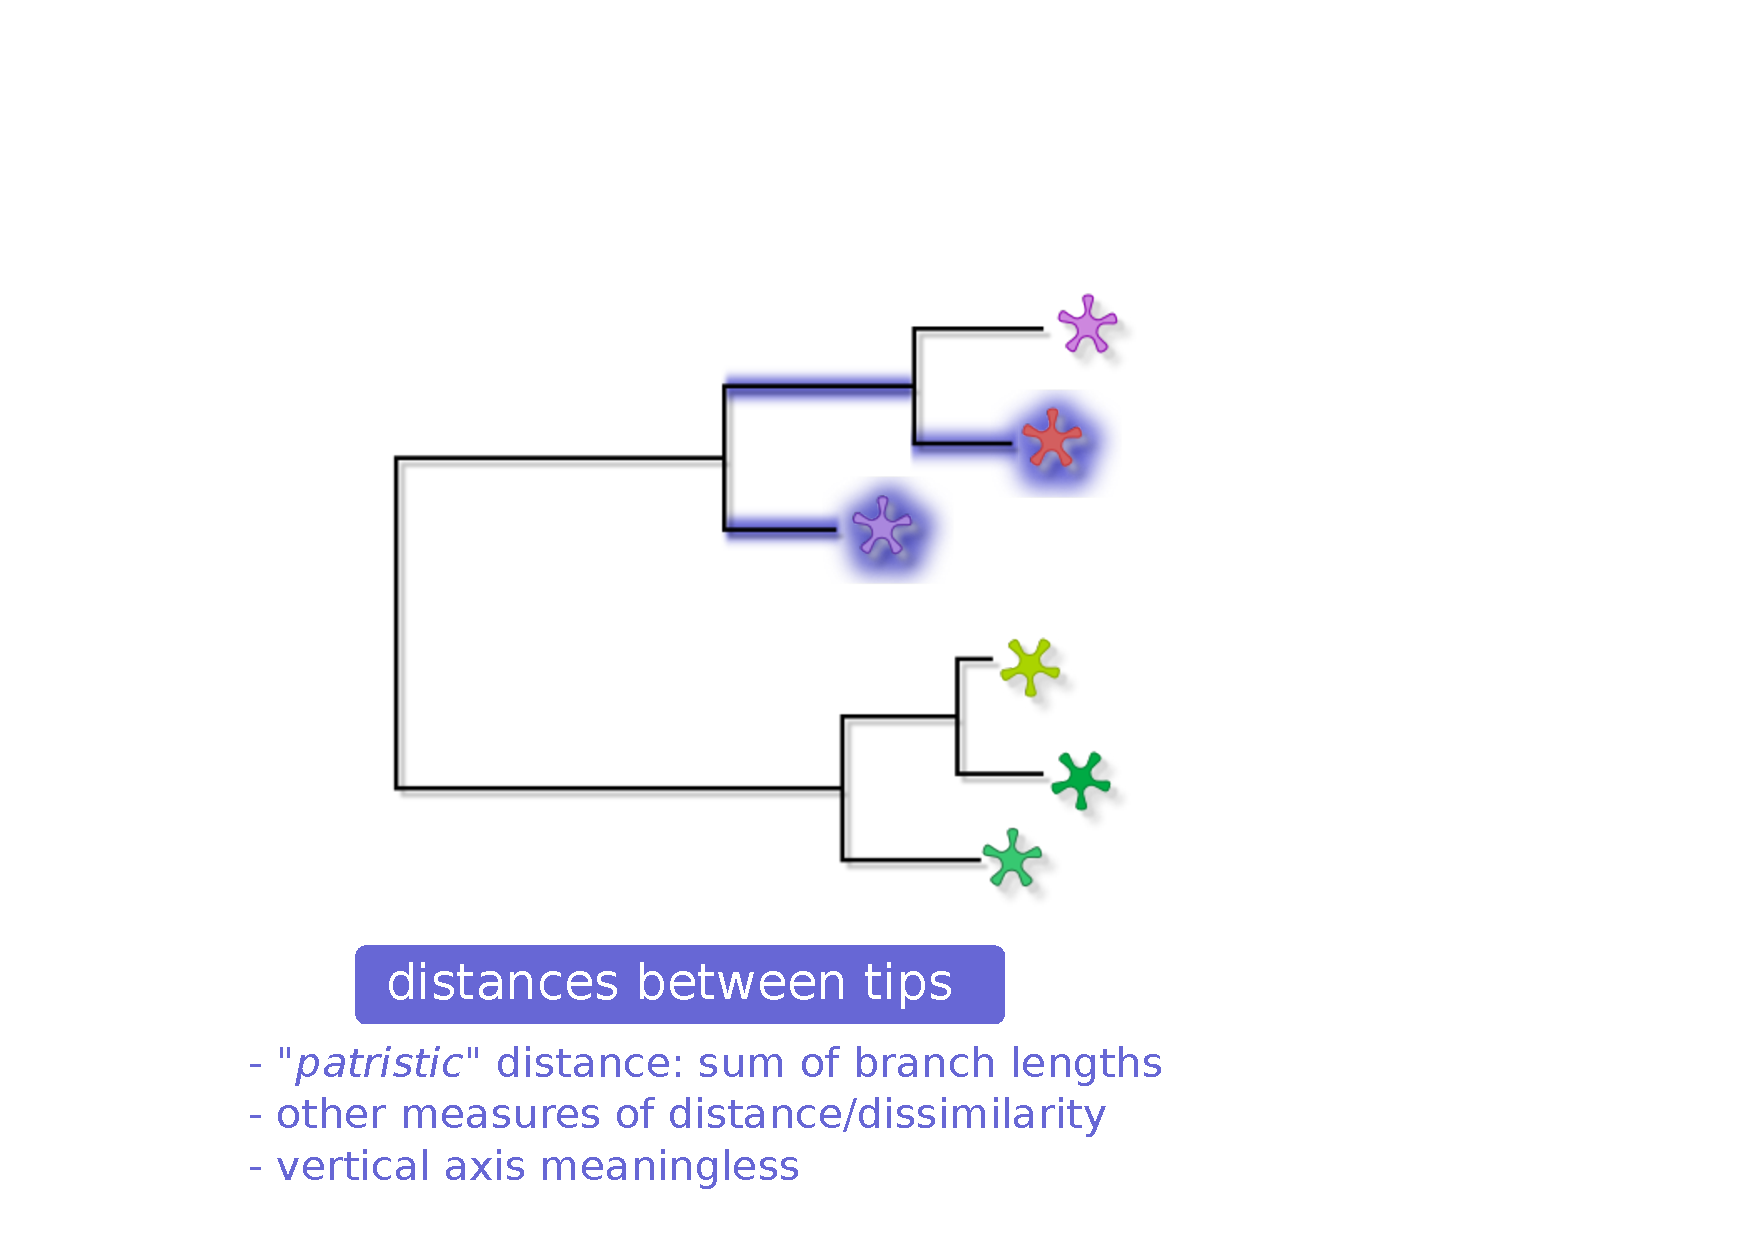
\includegraphics{figs/treeItemsDistances}}}\only<6->{\resizebox{\textwidth}{!}{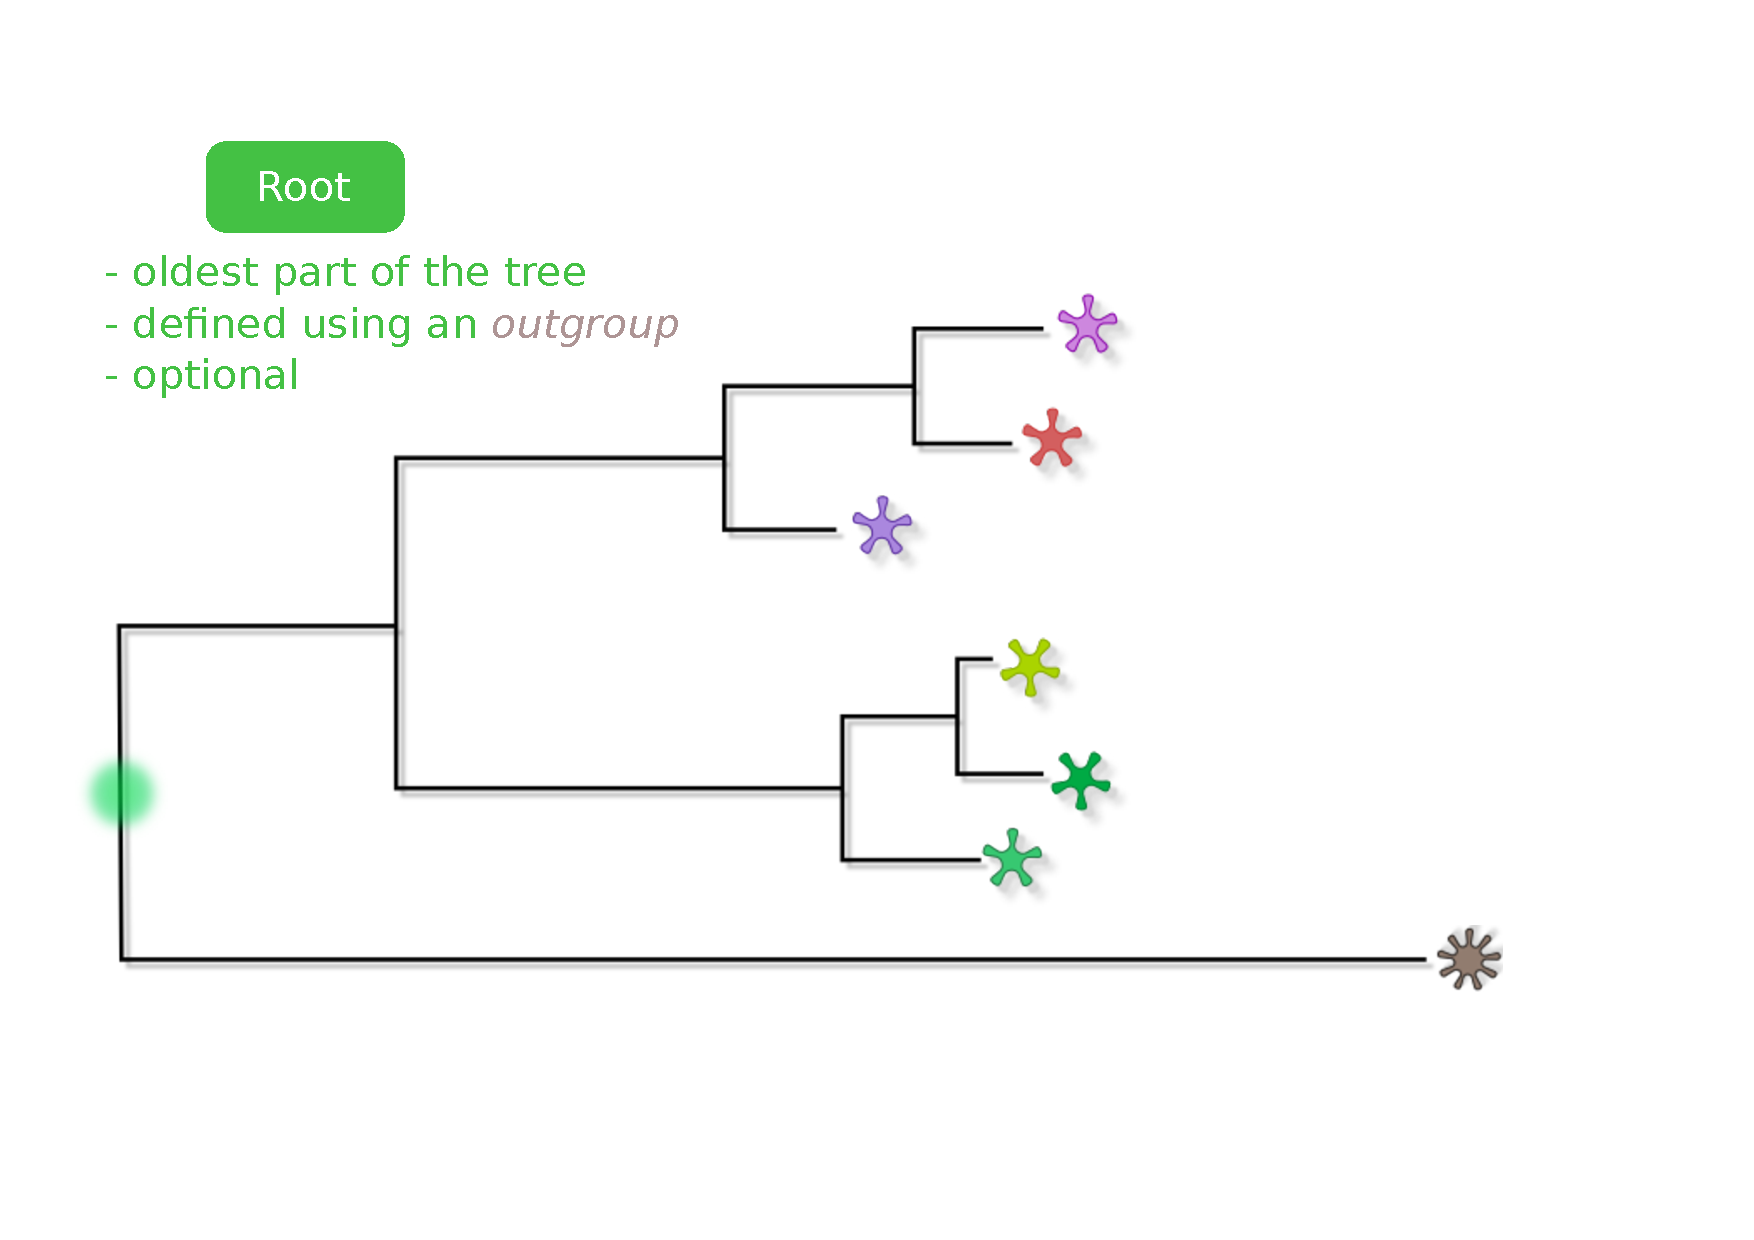
\includegraphics{figs/treeItemsRoot}}}

\visible<7->{How to we build them?}
\end{center}

\end{frame}
%%%%%%%%%%%%%%%%%%%%
%%%%%%%%%%%%%%%%%%%%





%%%%%%%%%%%%%%%%%%%%
%%%%%%%%%%%%%%%%%%%%
\begin{frame}
  \frametitle{Workflow}
\footnotesize
\begin{block}{Prepare data}
\begin{itemize}
   \item align sequences: alignment software + manual refinement
\end{itemize}
\end{block}

\pause

\begin{block}{\textbf<4->{Build the tree}}
\begin{itemize}
  \item \textbf<4->{distance-based methods}
  \item \textbf<4->{maximum parsimony}
  \item \textbf<4->{likelihood-based methods (ML, Bayesian)}
\end{itemize}
\end{block}

\pause

\begin{block}{Analyse the tree}
\begin{itemize}
  \item assess uncertainty
  \item test phylogenetic signal
  \item model trait evolution
  \item ...
\end{itemize}
\end{block}

\end{frame}







%%%%%%%%%%%%%%%%%%%%
%%%%%%%%%%%%%%%%%%%%
\section{Distance trees}
\subsection{~}
%%%%%%%%%%%%%%%%%%%%
%%%%%%%%%%%%%%%%%%%%


%%%%%%%%%%%%%%%%%%%%
%%%%%%%%%%%%%%%%%%%%
\begin{frame}
  \frametitle{Distance-based phylogenetic reconstruction}

Approaches relying on \textbf{agglomerative clustering} algorithms \\
(e.g. Single linkage, UPGMA, Neighbor-Joining)

\begin{block}{Rationale}
\begin{enumerate}
  \item compute pairwise genetic distances $\m{D}$
  \item group closest sequences
  \item update $\m{D}$
  \item go back to 2) until all sequences are grouped
\end{enumerate}
\end{block}

\end{frame}

%%%%%%%%%%%%%%%%%%%%
%%%%%%%%%%%%%%%%%%%%





%%%%%%%%%%%%%%%%%%%%
%%%%%%%%%%%%%%%%%%%%
\begin{frame}
  \frametitle{Distance-based phylogenetic reconstruction}


\begin{center}
    \only<1>{\resizebox{.8\textwidth}{!}{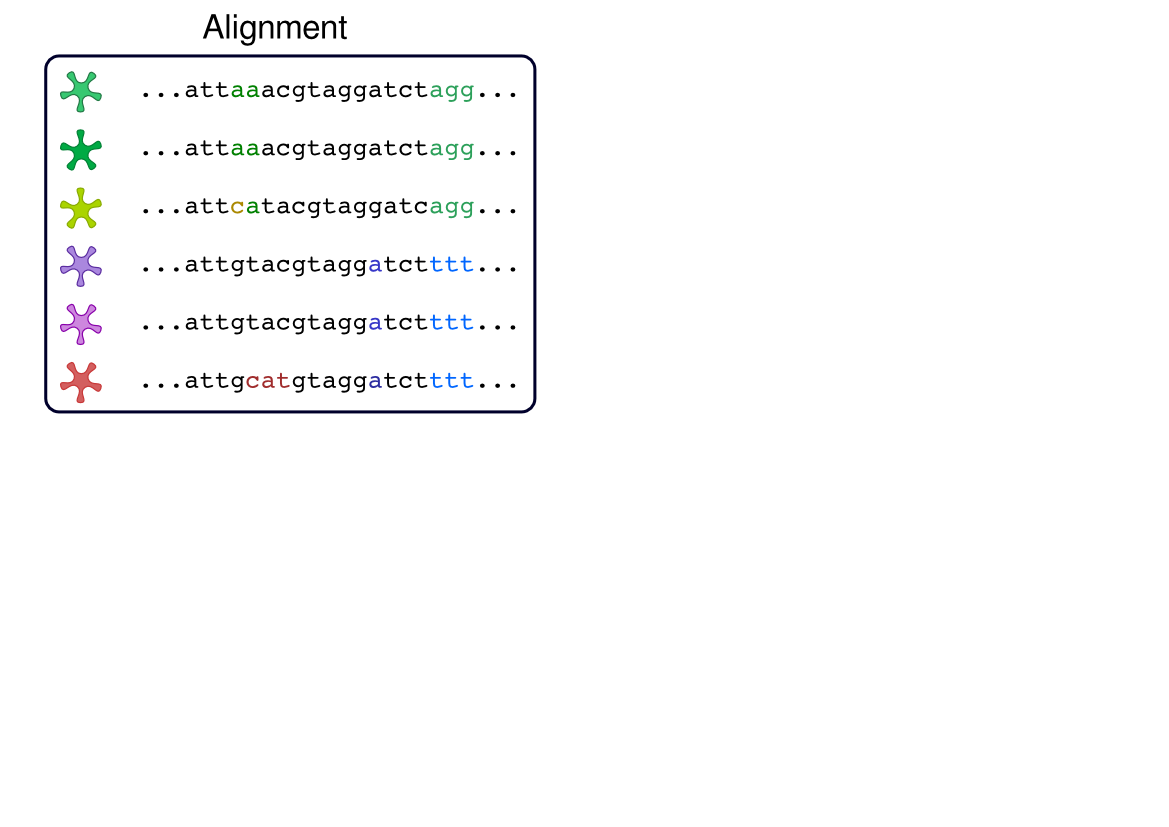
\includegraphics{figs/clustering1}}}\only<2>{\resizebox{.8\textwidth}{!}{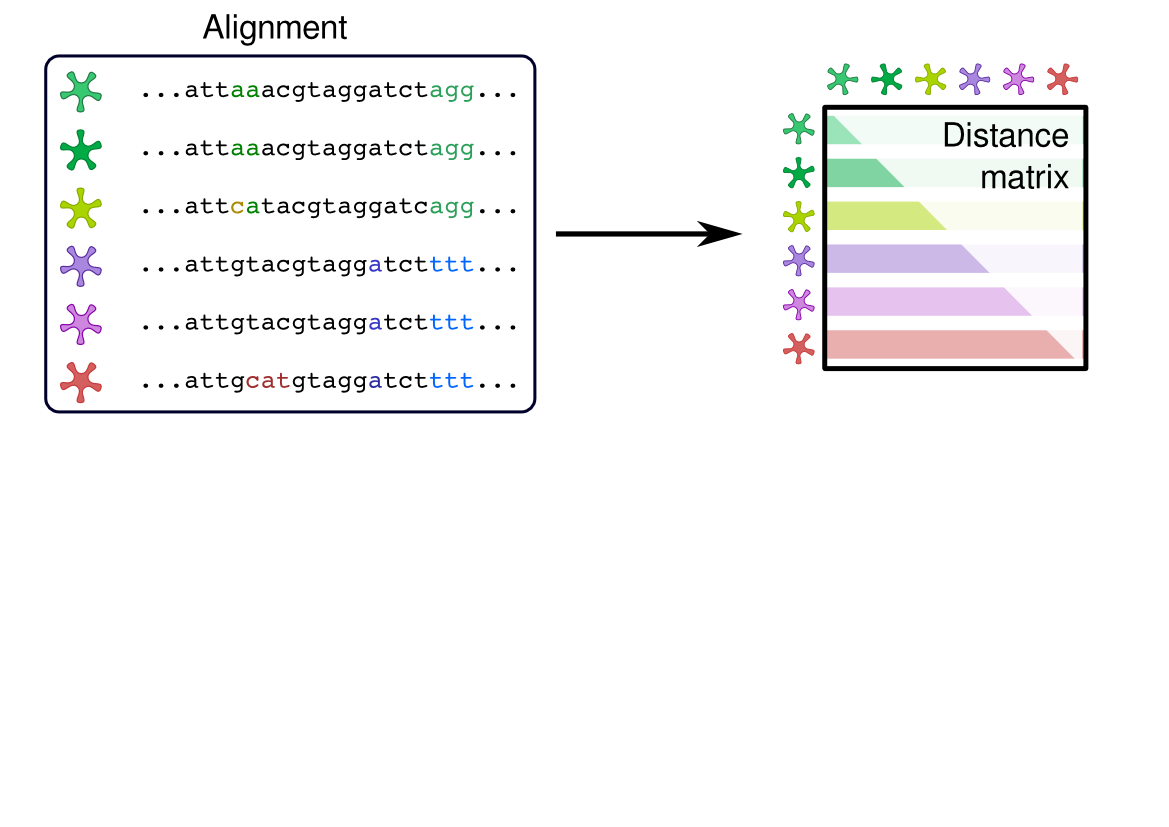
\includegraphics{figs/clustering2}}}\only<3>{\resizebox{.8\textwidth}{!}{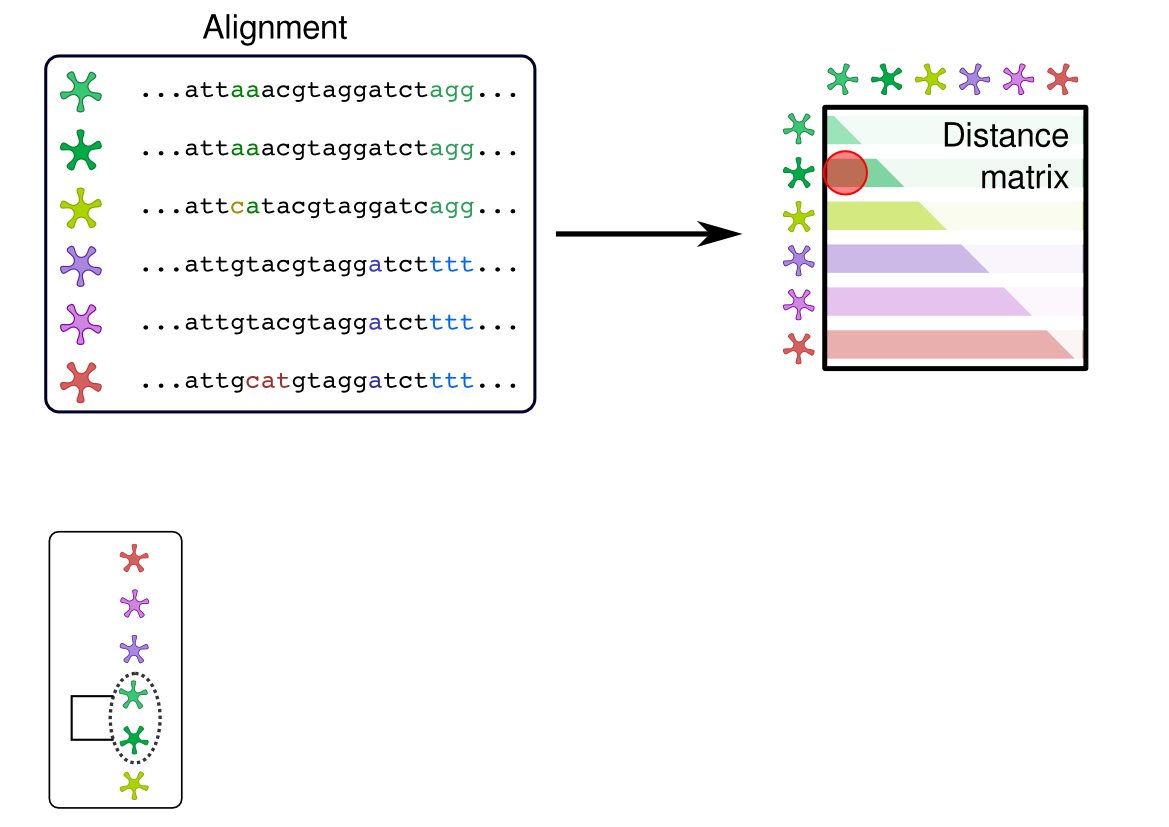
\includegraphics{figs/clustering3}}}\only<4>{\resizebox{.8\textwidth}{!}{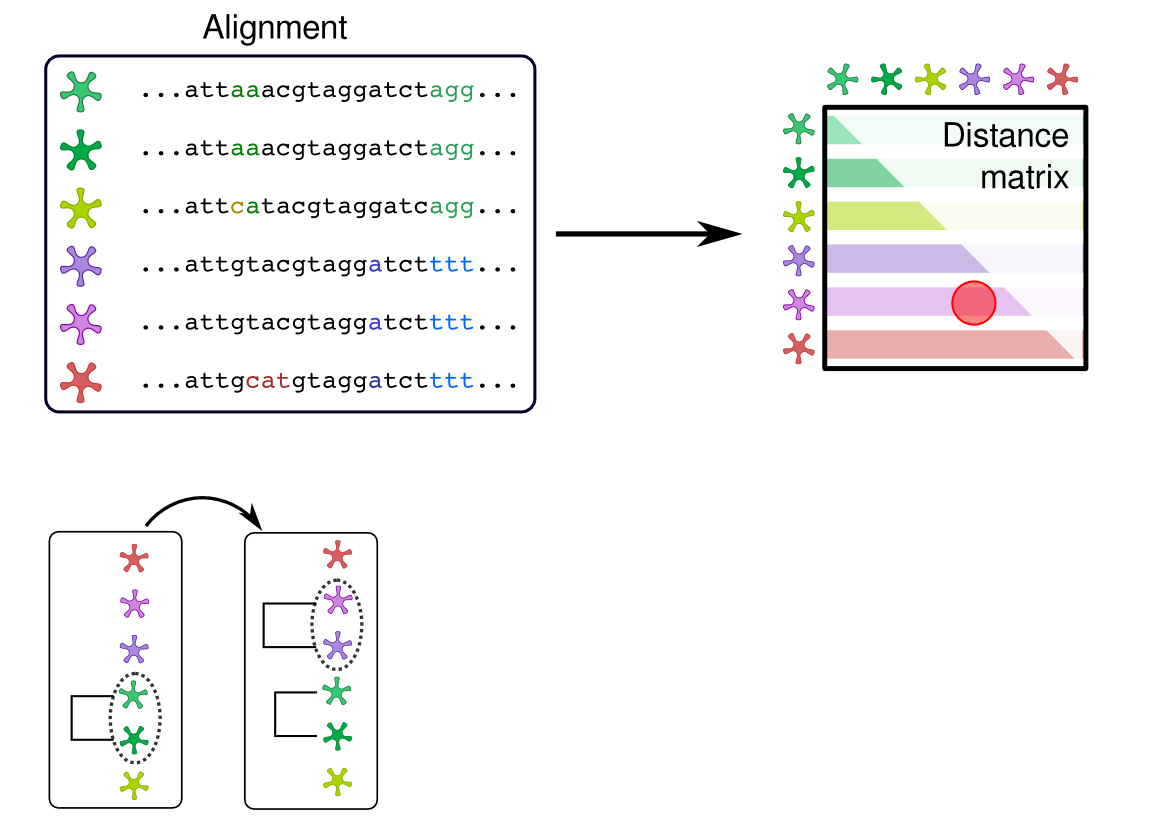
\includegraphics{figs/clustering4}}}\only<5>{\resizebox{.8\textwidth}{!}{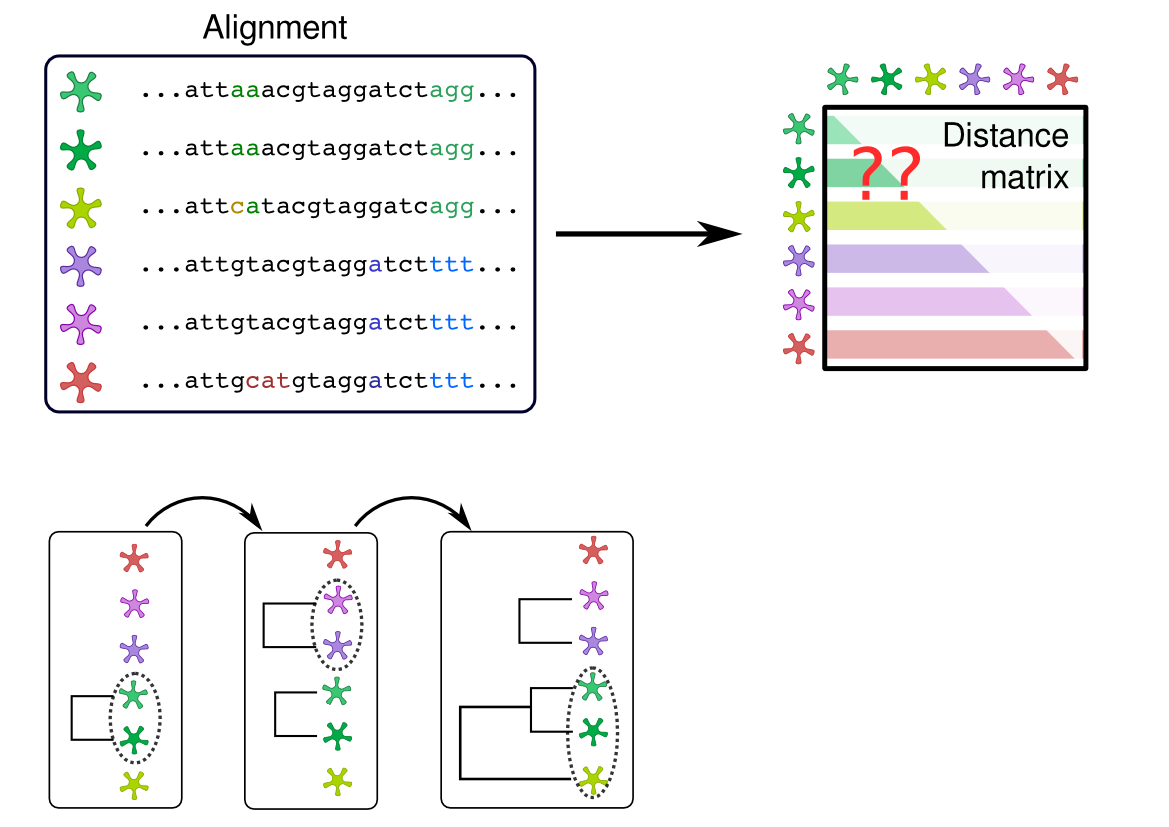
\includegraphics{figs/clustering5}}}\only<6->{\resizebox{.8\textwidth}{!}{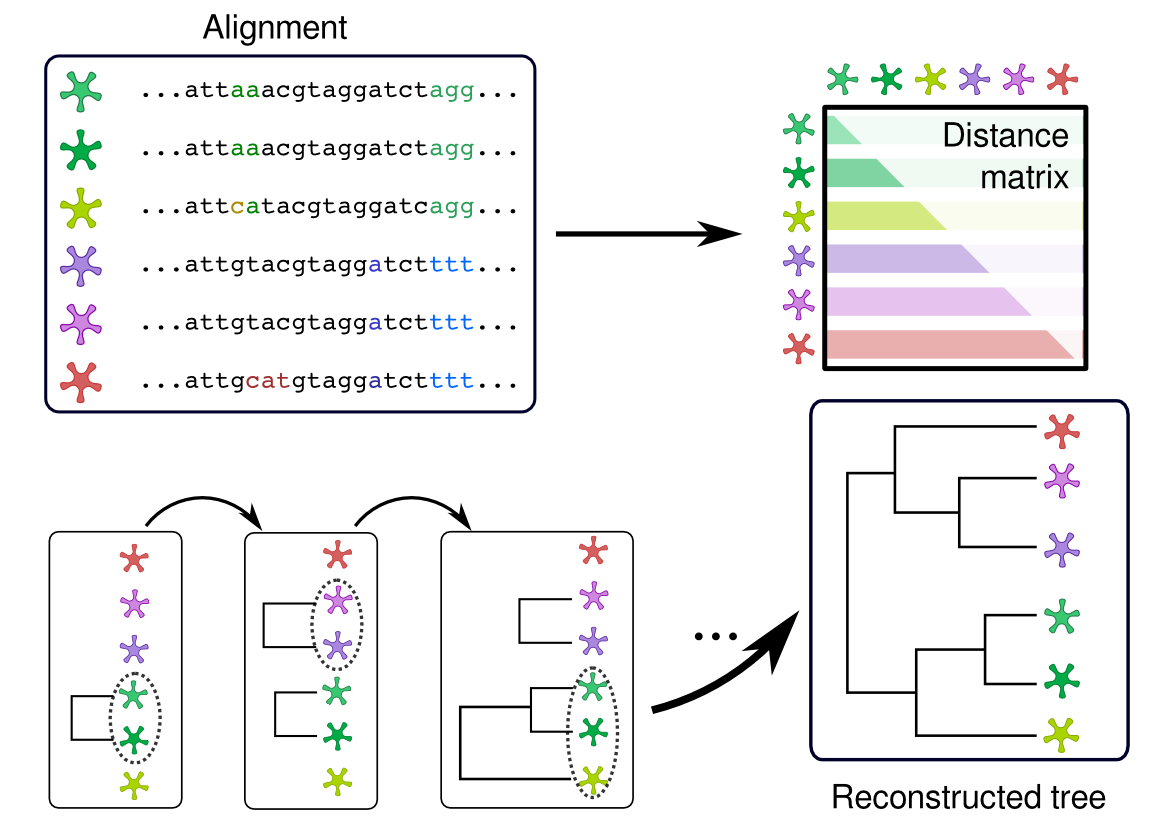
\includegraphics{figs/clustering6}}}
\end{center}

\end{frame}
%%%%%%%%%%%%%%%%%%%%
%%%%%%%%%%%%%%%%%%%%






%%%%%%%%%%%%%%%%%%%%%%%%%%%%
%%%%%%%%%%%%%%%%%%%%%%%%%%%%
\begin{frame}[fragile]
  \frametitle{What is the distance between a node and tips?}
  
\textbf{Hierarchical clustering:}
\vspace{.5cm}

  \begin{columns}[l]
    \column{0.3\textwidth}
     \resizebox{\textwidth}{!}{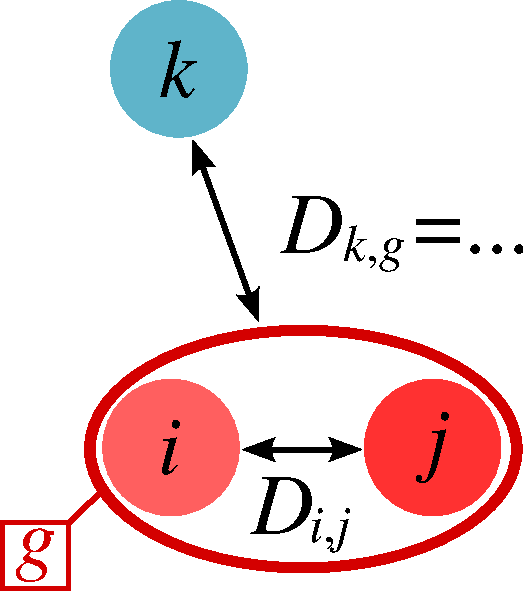
\includegraphics{figs/hclust2}}
    \column{0.7\textwidth}
    \pause
    \begin{itemize}
    \item single linkage: $D_{k,g} = \mbox{min}(D_{k,i}, D_{k,j})$ \pause
      ~\\
      ~\\

    \item complete linkage: $D_{k,g} = \mbox{max}(D_{k,i}, D_{k,j})$ \pause

      ~\\
    \item UPGMA: $D_{k,g} = \frac{D_{k,i} + D_{k,j}}{2}$
    \end{itemize}
  \end{columns}
\vspace{1cm}
 \pause
 \textbf{Neighbor joining:}
 
 
 Transforms original distances to account for heterogeneous rates of evolution.
 
\end{frame}
%%%%%%%%%%%%%%%%%%%%%%%%%%%%
%%%%%%%%%%%%%%%%%%%%%%%%%%%%





%%%%%%%%%%%%%%%%%%%%
%%%%%%%%%%%%%%%%%%%%
\begin{frame}
  \frametitle{Distance-based phylogenetic reconstruction}

\begin{block}{Advantages}
\begin{itemize}
 \item simple
 \item flexible (many distances and clustering algorithms)
 \item fast and scalable (applicable to large datasets)
\end{itemize}
\end{block}

\pause

\begin{block}{Limitations}
\begin{itemize}
 \item sensitive to distance/clustering chosen
 \item evolutionary rates are not estimated
 \item no measure of uncertainty for the tree obtained
\end{itemize}
\end{block}

\end{frame}

%%%%%%%%%%%%%%%%%%%%
%%%%%%%%%%%%%%%%%%%%







%%%%%%%%%%%%%%%%%%%%
%%%%%%%%%%%%%%%%%%%%
\section{Parsimony}
\subsection{~}
%%%%%%%%%%%%%%%%%%%%
%%%%%%%%%%%%%%%%%%%%


%%%%%%%%%%%%%%%%%%%%
%%%%%%%%%%%%%%%%%%%%
\begin{frame}
  \frametitle{Maximum parsimony phylogenies}

\vspace{-.5cm}
Approaches relying on finding the tree with the \textbf{smallest number of character changes (substitutions)}
\vspace{.25cm}

\begin{block}{Rationale}
\begin{enumerate}
  \item start from a pre-defined tree
  \item compute initial parsimony score
  \item permute branches and compute parsimony score
  \item accept new tree if the parsimony score is improved
  \item go back to 3) until convergence
\end{enumerate}
\end{block}

\end{frame}




%%%%%%%%%%%%%%%%%%%%
%%%%%%%%%%%%%%%%%%%%
\begin{frame}
  \frametitle{Maximum parsimony phylogenies}

\begin{center}
    \only<1>{\resizebox{\textwidth}{!}{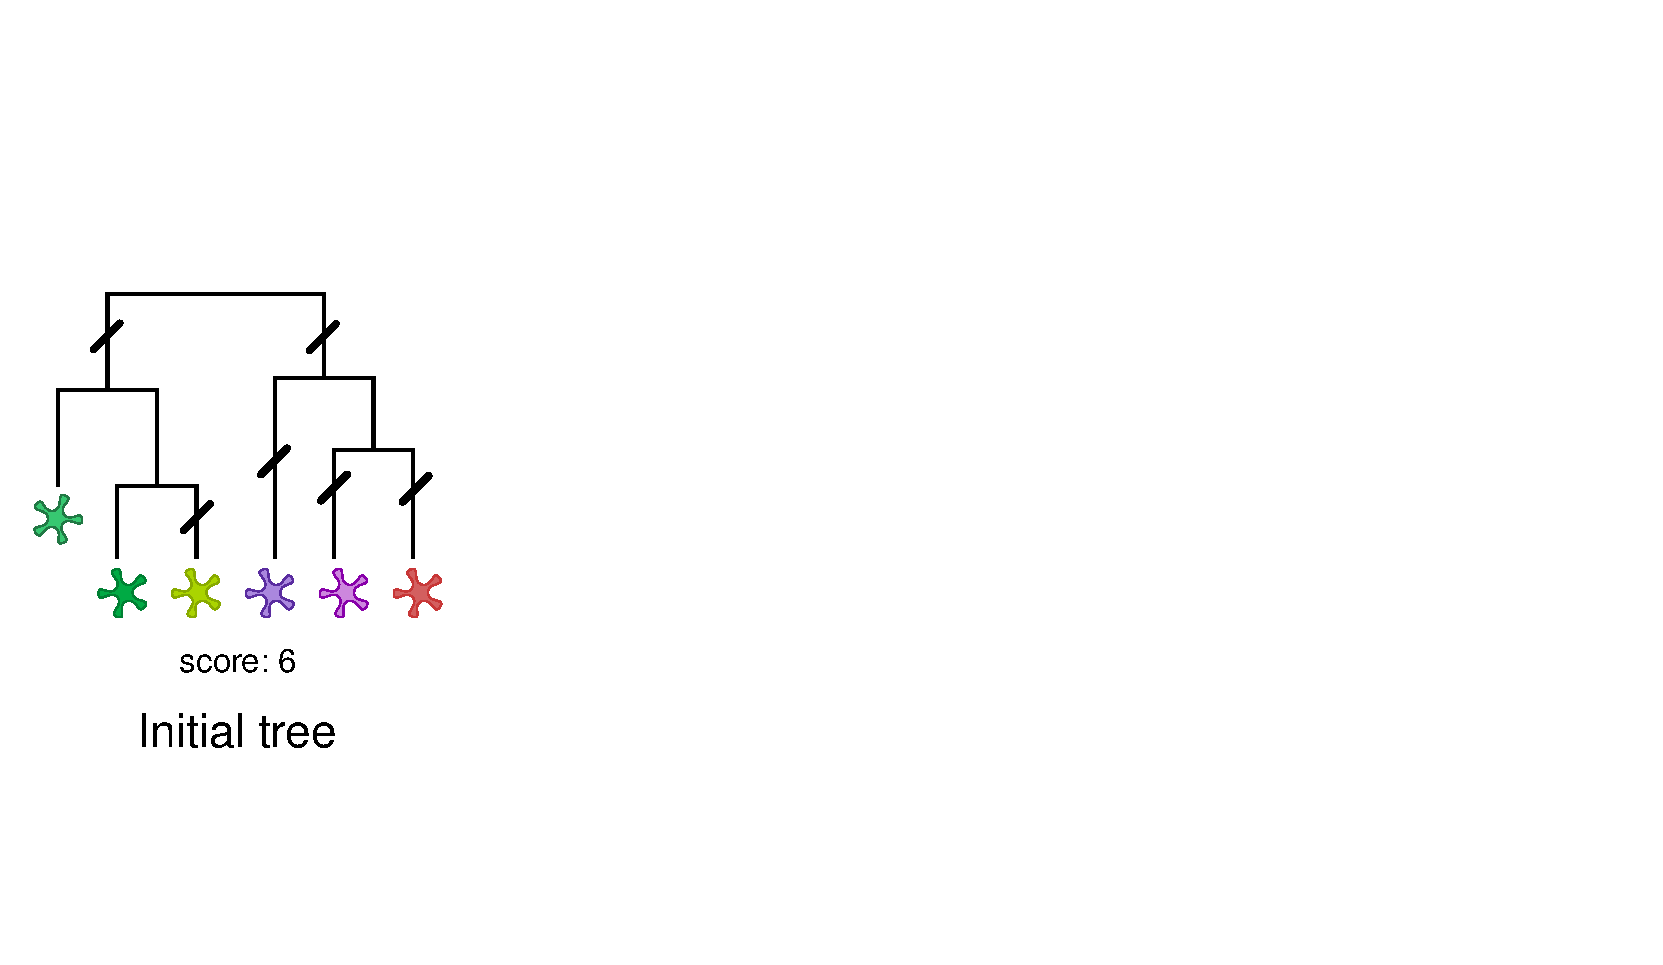
\includegraphics{figs/parsimony1}}}\only<2>{\resizebox{\textwidth}{!}{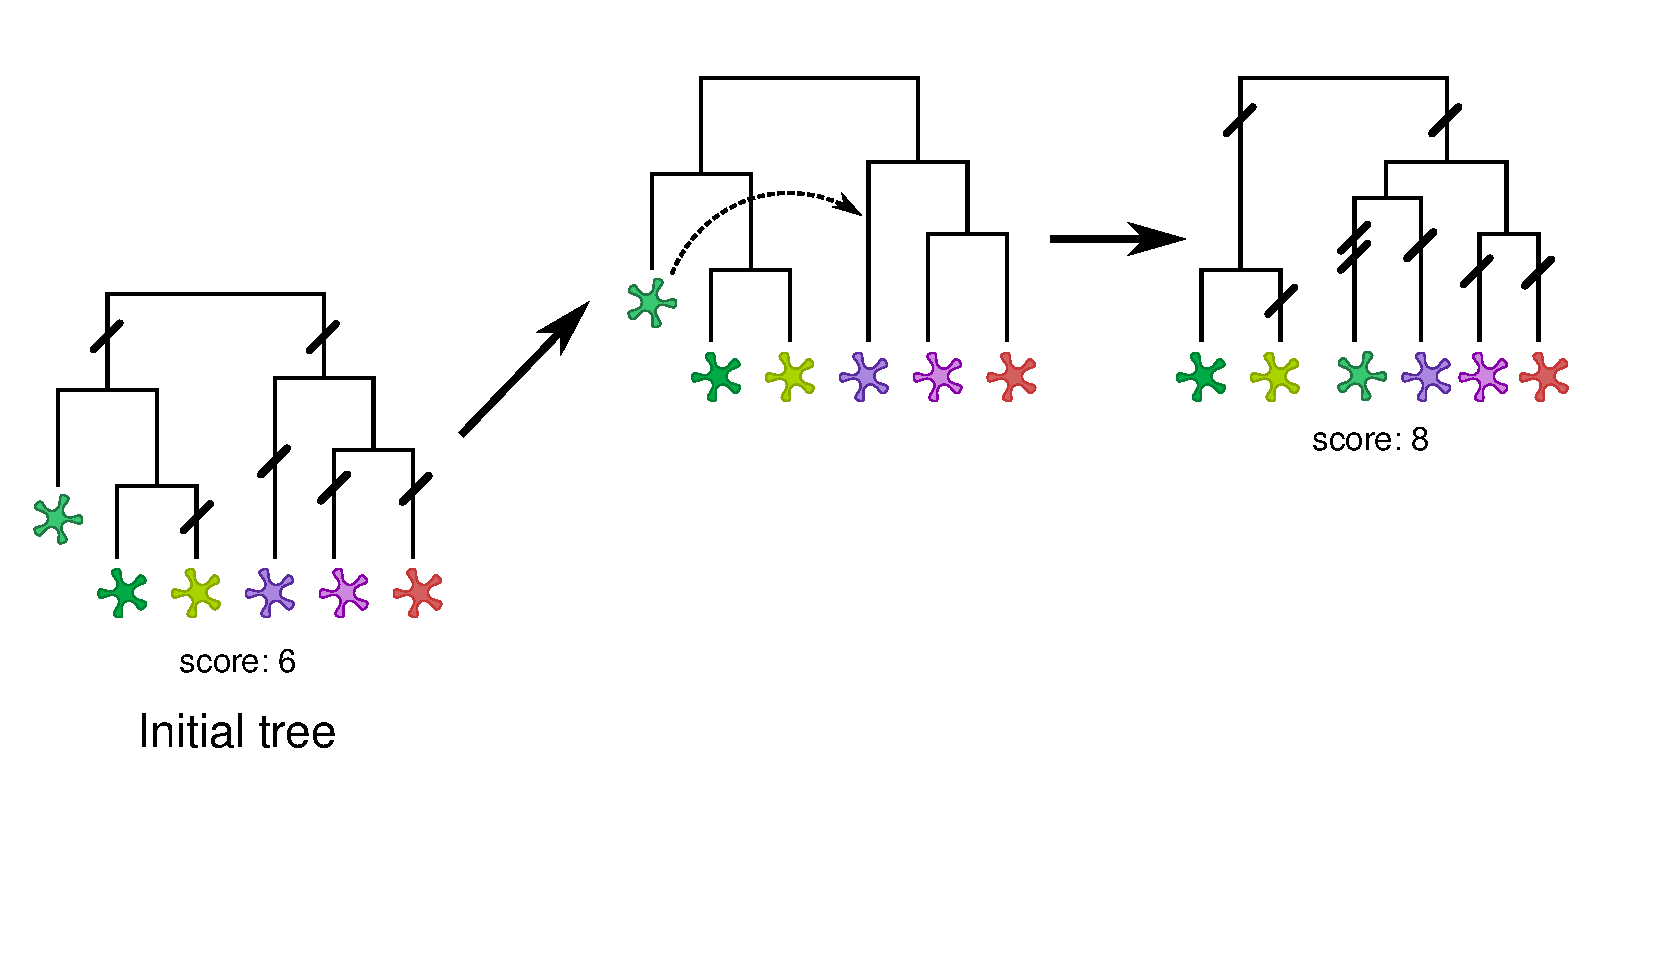
\includegraphics{figs/parsimony2}}}\only<3>{\resizebox{\textwidth}{!}{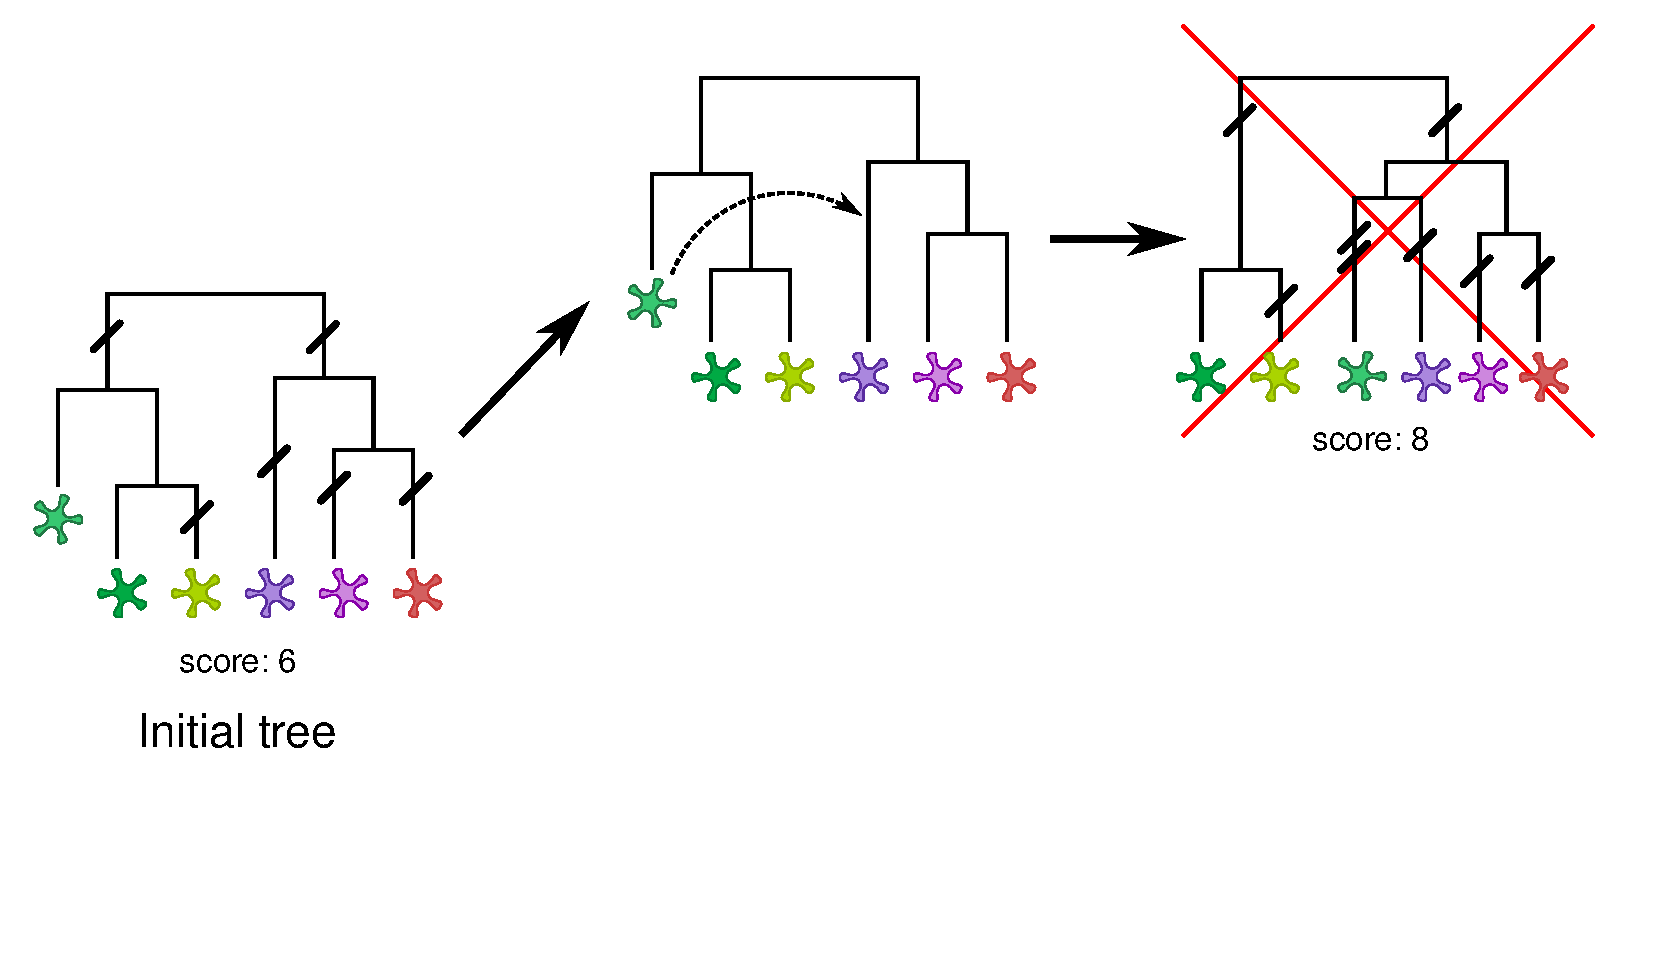
\includegraphics{figs/parsimony3}}}\only<4>{\resizebox{\textwidth}{!}{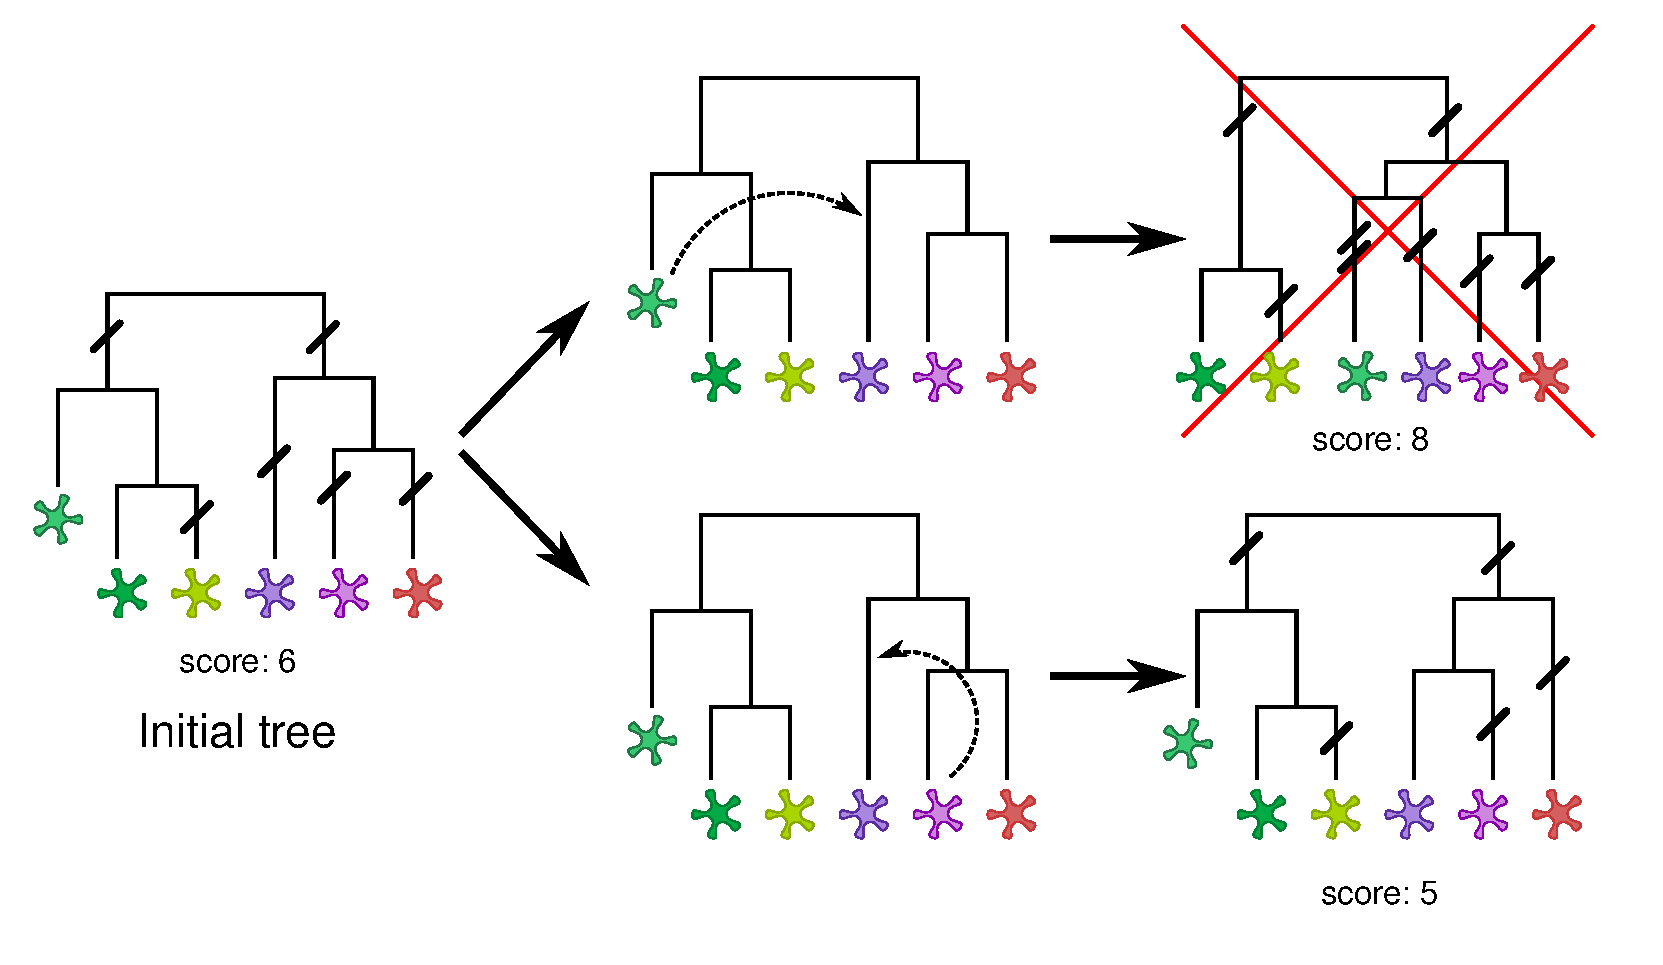
\includegraphics{figs/parsimony4}}}\only<5->{\resizebox{\textwidth}{!}{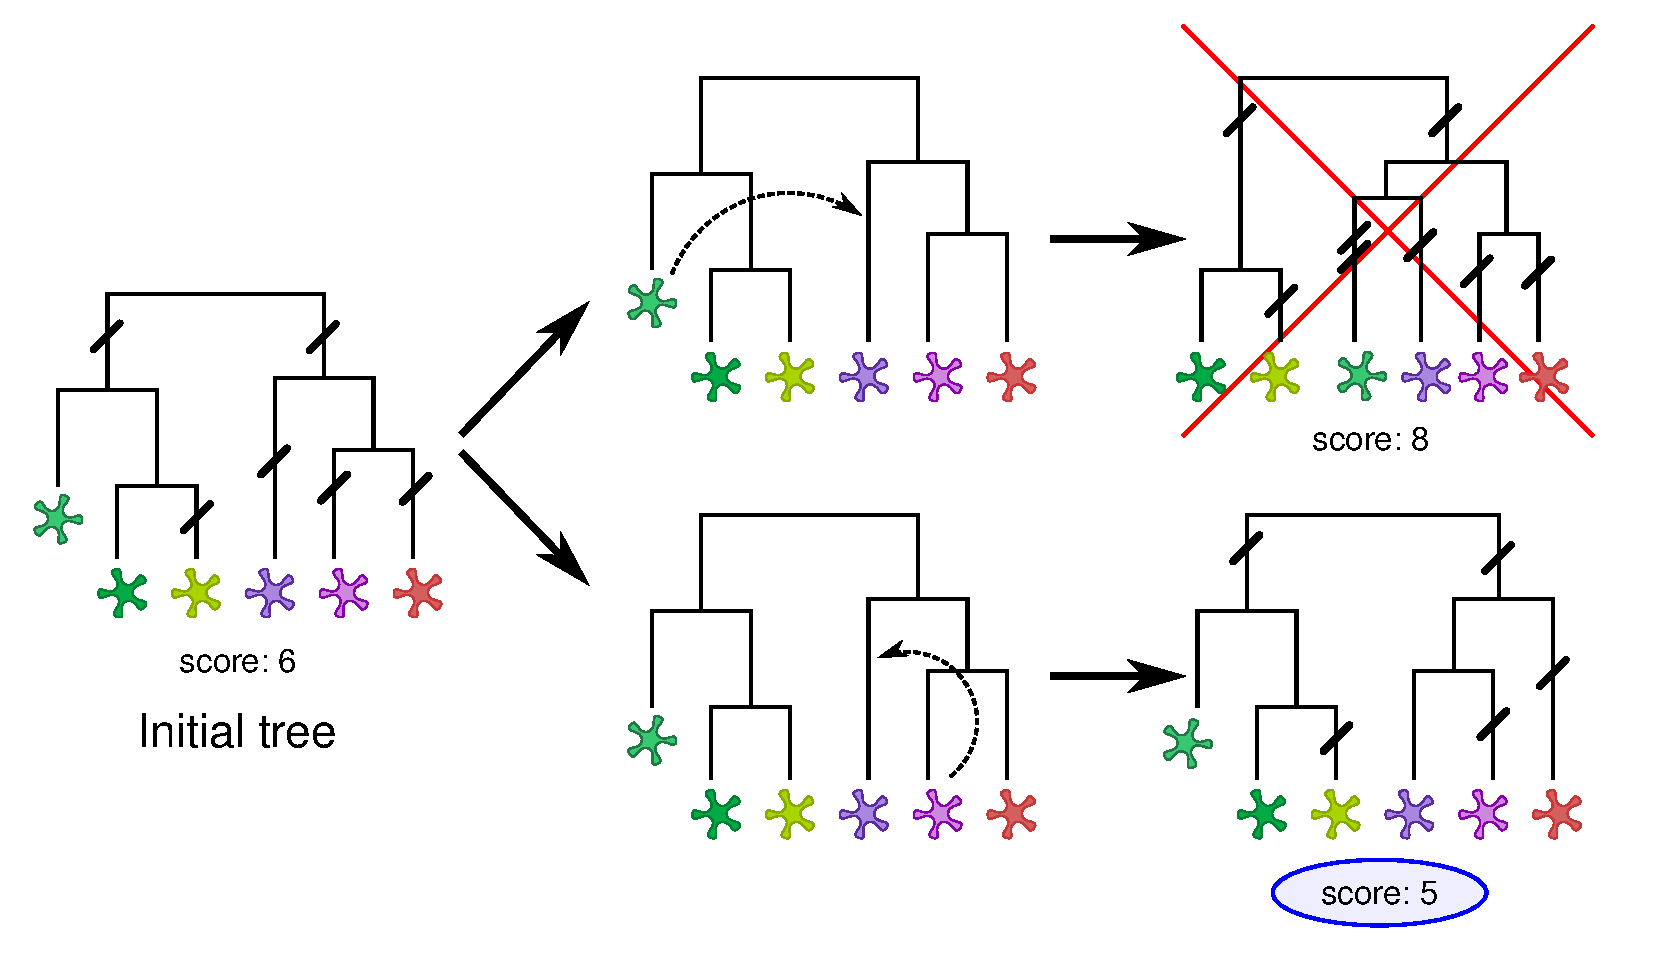
\includegraphics{figs/parsimony5}}}
\end{center}

\end{frame}




%%%%%%%%%%%%%%%%%%%%
%%%%%%%%%%%%%%%%%%%%
\begin{frame}
  \frametitle{Maximum parsimony phylogenies}

\begin{block}{Advantages}
\begin{itemize}
 \item applicable to any discontinuous characters (not just DNA)
 \item intuitive explanation: `simplest' evolutionary scenario
\end{itemize}
\end{block}

\pause

\begin{block}{Limitations}
\begin{itemize}
 \item evolutionary rates are not estimated
 \item no measure of uncertainty for the tree obtained
 \item computer-intensive
 \item different types of substitutions ignored
 \item evolution not necessarily parsimonious
 \item sensitive to heterogeneous rates of evolution (\textit{long branch attraction})
\end{itemize}
\end{block}

\end{frame}






%%%%%%%%%%%%%%%%%%%%
%%%%%%%%%%%%%%%%%%%%
\section{Likelihood/Bayesian}
\subsection{~}
%%%%%%%%%%%%%%%%%%%%
%%%%%%%%%%%%%%%%%%%%


%%%%%%%%%%%%%%%%%%%%
%%%%%%%%%%%%%%%%%%%%
\begin{frame}
  \frametitle{Likelihood-based phylogenies (ML / Bayesian)}

Approaches relying on a \textbf{model of sequence evolution}:
\begin{itemize}
 \item \textbf{ML}: find tree and evolutionary rates with highest likelihood
 \item \textbf{Bayesian}: find tree and evolutionary rates to posterior probability
\end{itemize}

\pause

\begin{block}{Rationale}
\begin{enumerate}
  \item start from a pre-defined tree
  \item compute initial likelihood/posterior
  \item permute branches, sample new parameters and compute likelihood/posterior
  \item accept new tree and parameters based on likelihood/posterior improvement
  \item go back to 3) until convergence
\end{enumerate}
\end{block}

\end{frame}




%%%%%%%%%%%%%%%%%%%%
%%%%%%%%%%%%%%%%%%%%
\begin{frame}
  \frametitle{Likelihood-based phylogenies (ML / Bayesian)}

\begin{center}
    \only<1->{\resizebox{\textwidth}{!}{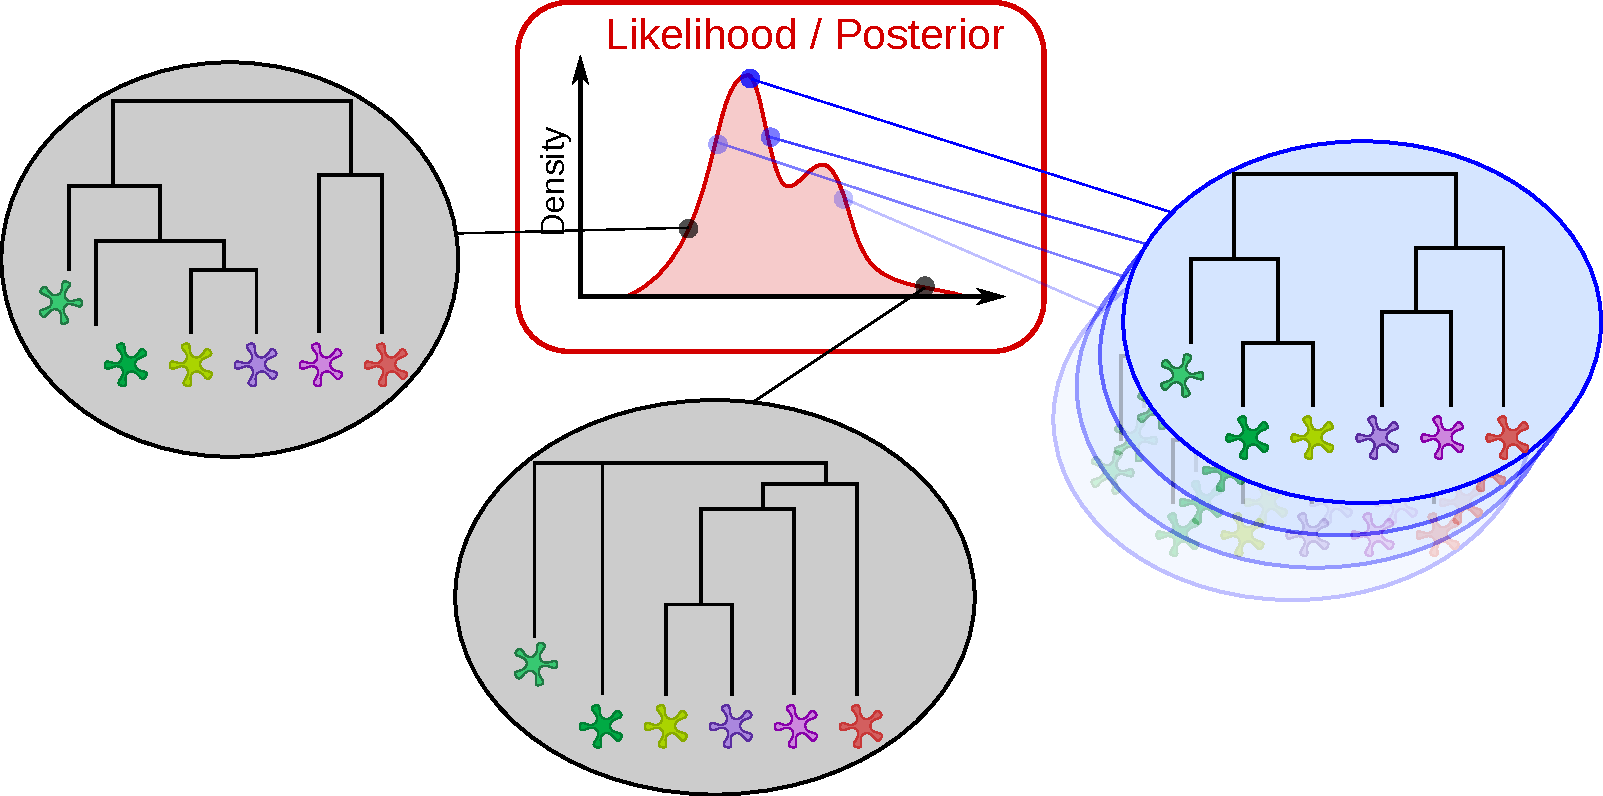
\includegraphics{figs/phyloML}}}
\end{center}

\end{frame}




%%%%%%%%%%%%%%%%%%%%
%%%%%%%%%%%%%%%%%%%%
\begin{frame}
  \frametitle{Likelihood-based phylogenies (ML / Bayesian)}

\begin{block}{Advantages}
\begin{itemize}
 \item very flexible
 \item consistent with a model of evolution
 \item statistically consistent (model comparison)
 \item parameter estimation
 \item (Bayesian) several trees $\rightarrow$ measure of uncertainty
\end{itemize}
\end{block}

\pause

\begin{block}{Limitations}
\begin{itemize}
 \item computer-intensive
 \item choice of the model of evolution
 \item (ML) no measure of uncertainty for the tree obtained
 \item (Bayesian) need to find a consensus tree
\end{itemize}
\end{block}

\end{frame}










%%%%%%%%%%%%%%%%%%%%
%%%%%%%%%%%%%%%%%%%%
\section{Uncertainty}
\subsection{~}
%%%%%%%%%%%%%%%%%%%%
%%%%%%%%%%%%%%%%%%%%


%%%%%%%%%%%%%%%%%%%%
%%%%%%%%%%%%%%%%%%%%
\begin{frame}
  \frametitle{How do we know the tree is robust?}

\textbf{Main issue:} assess the uncertainty of the tree topology / individual nodes

\pause
  \begin{columns}[l]
    \column{0.6\textwidth}

\begin{block}{Approaches}
\begin{itemize}
 \item ML: model selection to compare trees (whole tree)\pause
 \item Bayesian methods: between-samples variability (individual nodes)\pause
 \item \textbf<5->{any method: \\bootstrap (individual nodes)}
\end{itemize}
\end{block}
    \column{0.4\textwidth}
    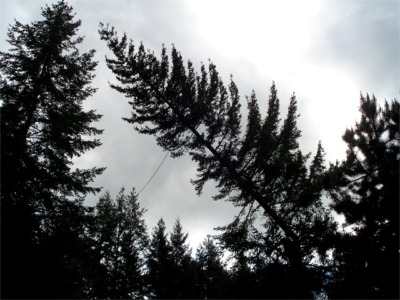
\includegraphics[width=\textwidth]{figs/treefall}
\end{columns}
\end{frame}




%%%%%%%%%%%%%%%%%%%%
%%%%%%%%%%%%%%%%%%%%
\begin{frame}
  \frametitle{Bootstrapping phylogenies}

\begin{itemize}
 \item assess \textbf{variability due to sampling the genome} and \textbf{conflicting signals}
 \item relies on analysing \textbf{resampled datasets}
\end{itemize}

\pause

\begin{block}{Rationale}
\begin{enumerate}
  \item obtain a reference tree
  \item resample the sites with replacement
  \item obtain a tree for the resampled dataset
  \item go back to 2) until the desired number of bootstrapped trees is attained
  \item compute the frequency of each bifurcation of the reference tree occuring in bootstrapped trees
\end{enumerate}
\end{block}

\end{frame}




%%%%%%%%%%%%%%%%%%%%
%%%%%%%%%%%%%%%%%%%%
\begin{frame}
  \frametitle{Bootstrapping phylogenies}

\begin{center}
    \only<1->{\resizebox{.8\textwidth}{!}{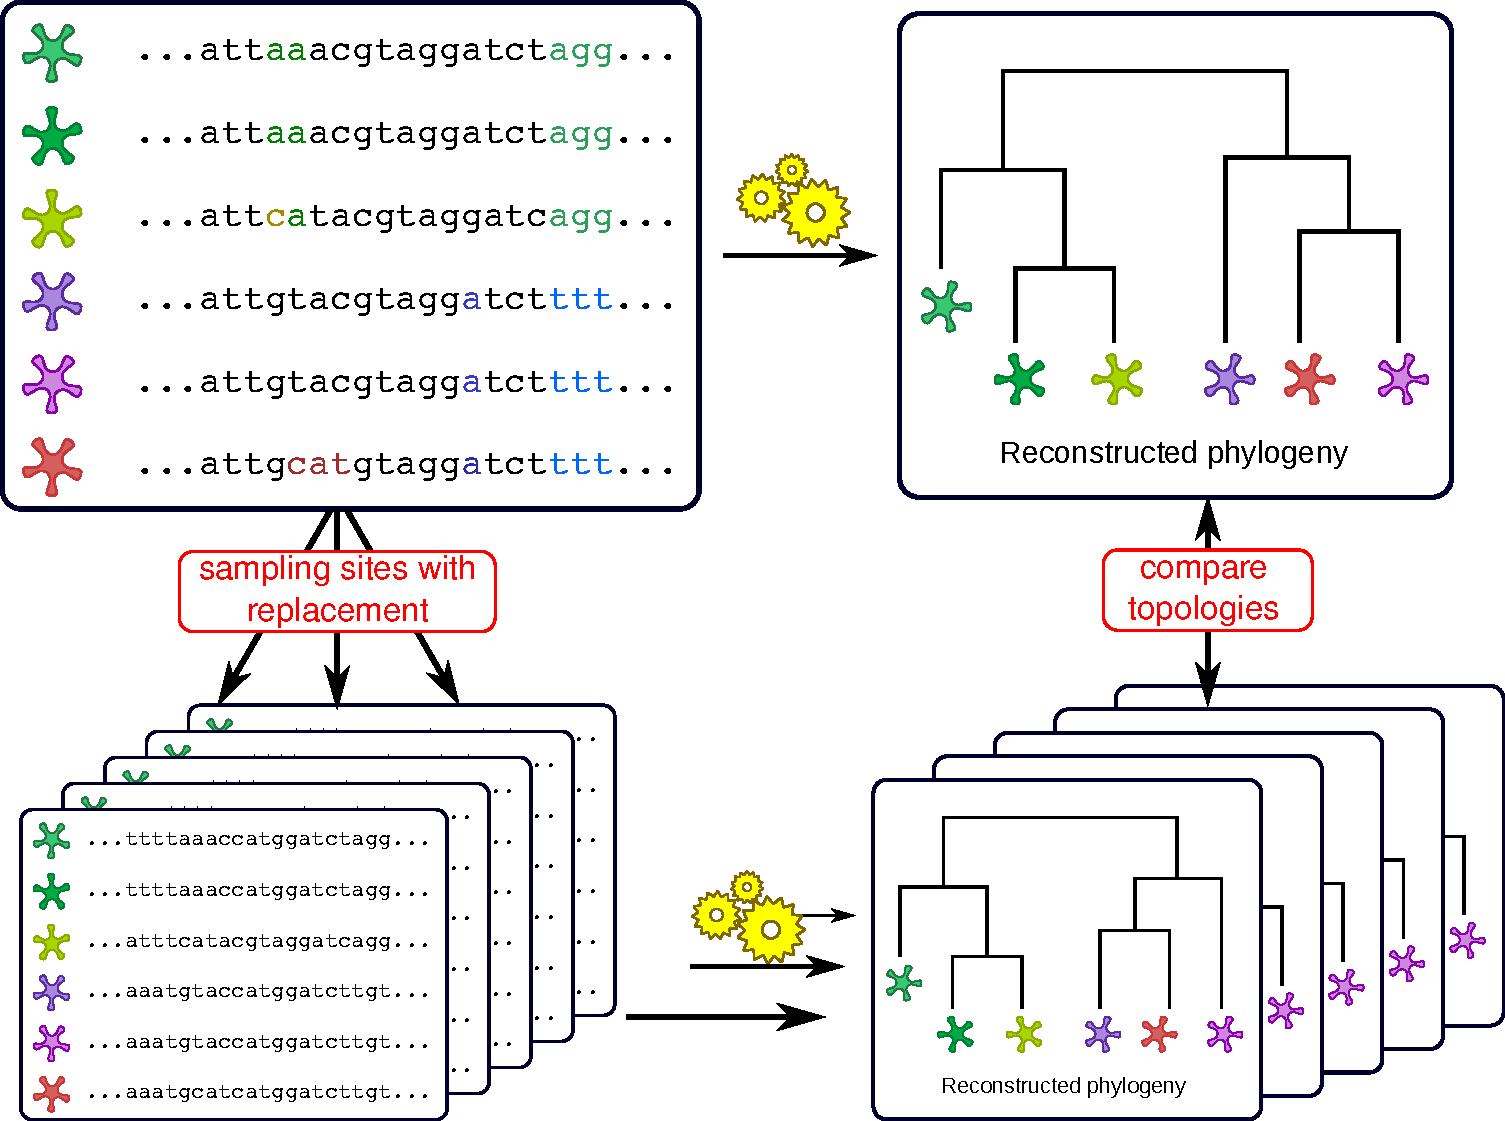
\includegraphics{figs/bootstrap}}}
\end{center}


\end{frame}





%%%%%%%%%%%%%%%%%%%%
%%%%%%%%%%%%%%%%%%%%
\begin{frame}
  \frametitle{Bootstrapping phylogenies}

\begin{block}{Advantages}
\begin{itemize}
 \item standard
 \item simple to implement
\end{itemize}
\end{block}

\pause

\begin{block}{Limitations}
\begin{itemize}
 \item possibly computer-intensive
 \item assumes that the genome has been sampled randomly (often wrong)
\end{itemize}
\end{block}

\end{frame}





%%%%%%%%%%%%%%%%%%%%
%%%%%%%%%%%%%%%%%%%%
\section{Pitfalls \& best practices}
\subsection{~}
%%%%%%%%%%%%%%%%%%%%
%%%%%%%%%%%%%%%%%%%%

%%%%%%%%%%%%%%%%%%%%
%%%%%%%%%%%%%%%%%%%%
\begin{frame}
  \frametitle{Plotting trees as rooted}

\begin{center}
    \only<1->{\resizebox{.9\textwidth}{!}{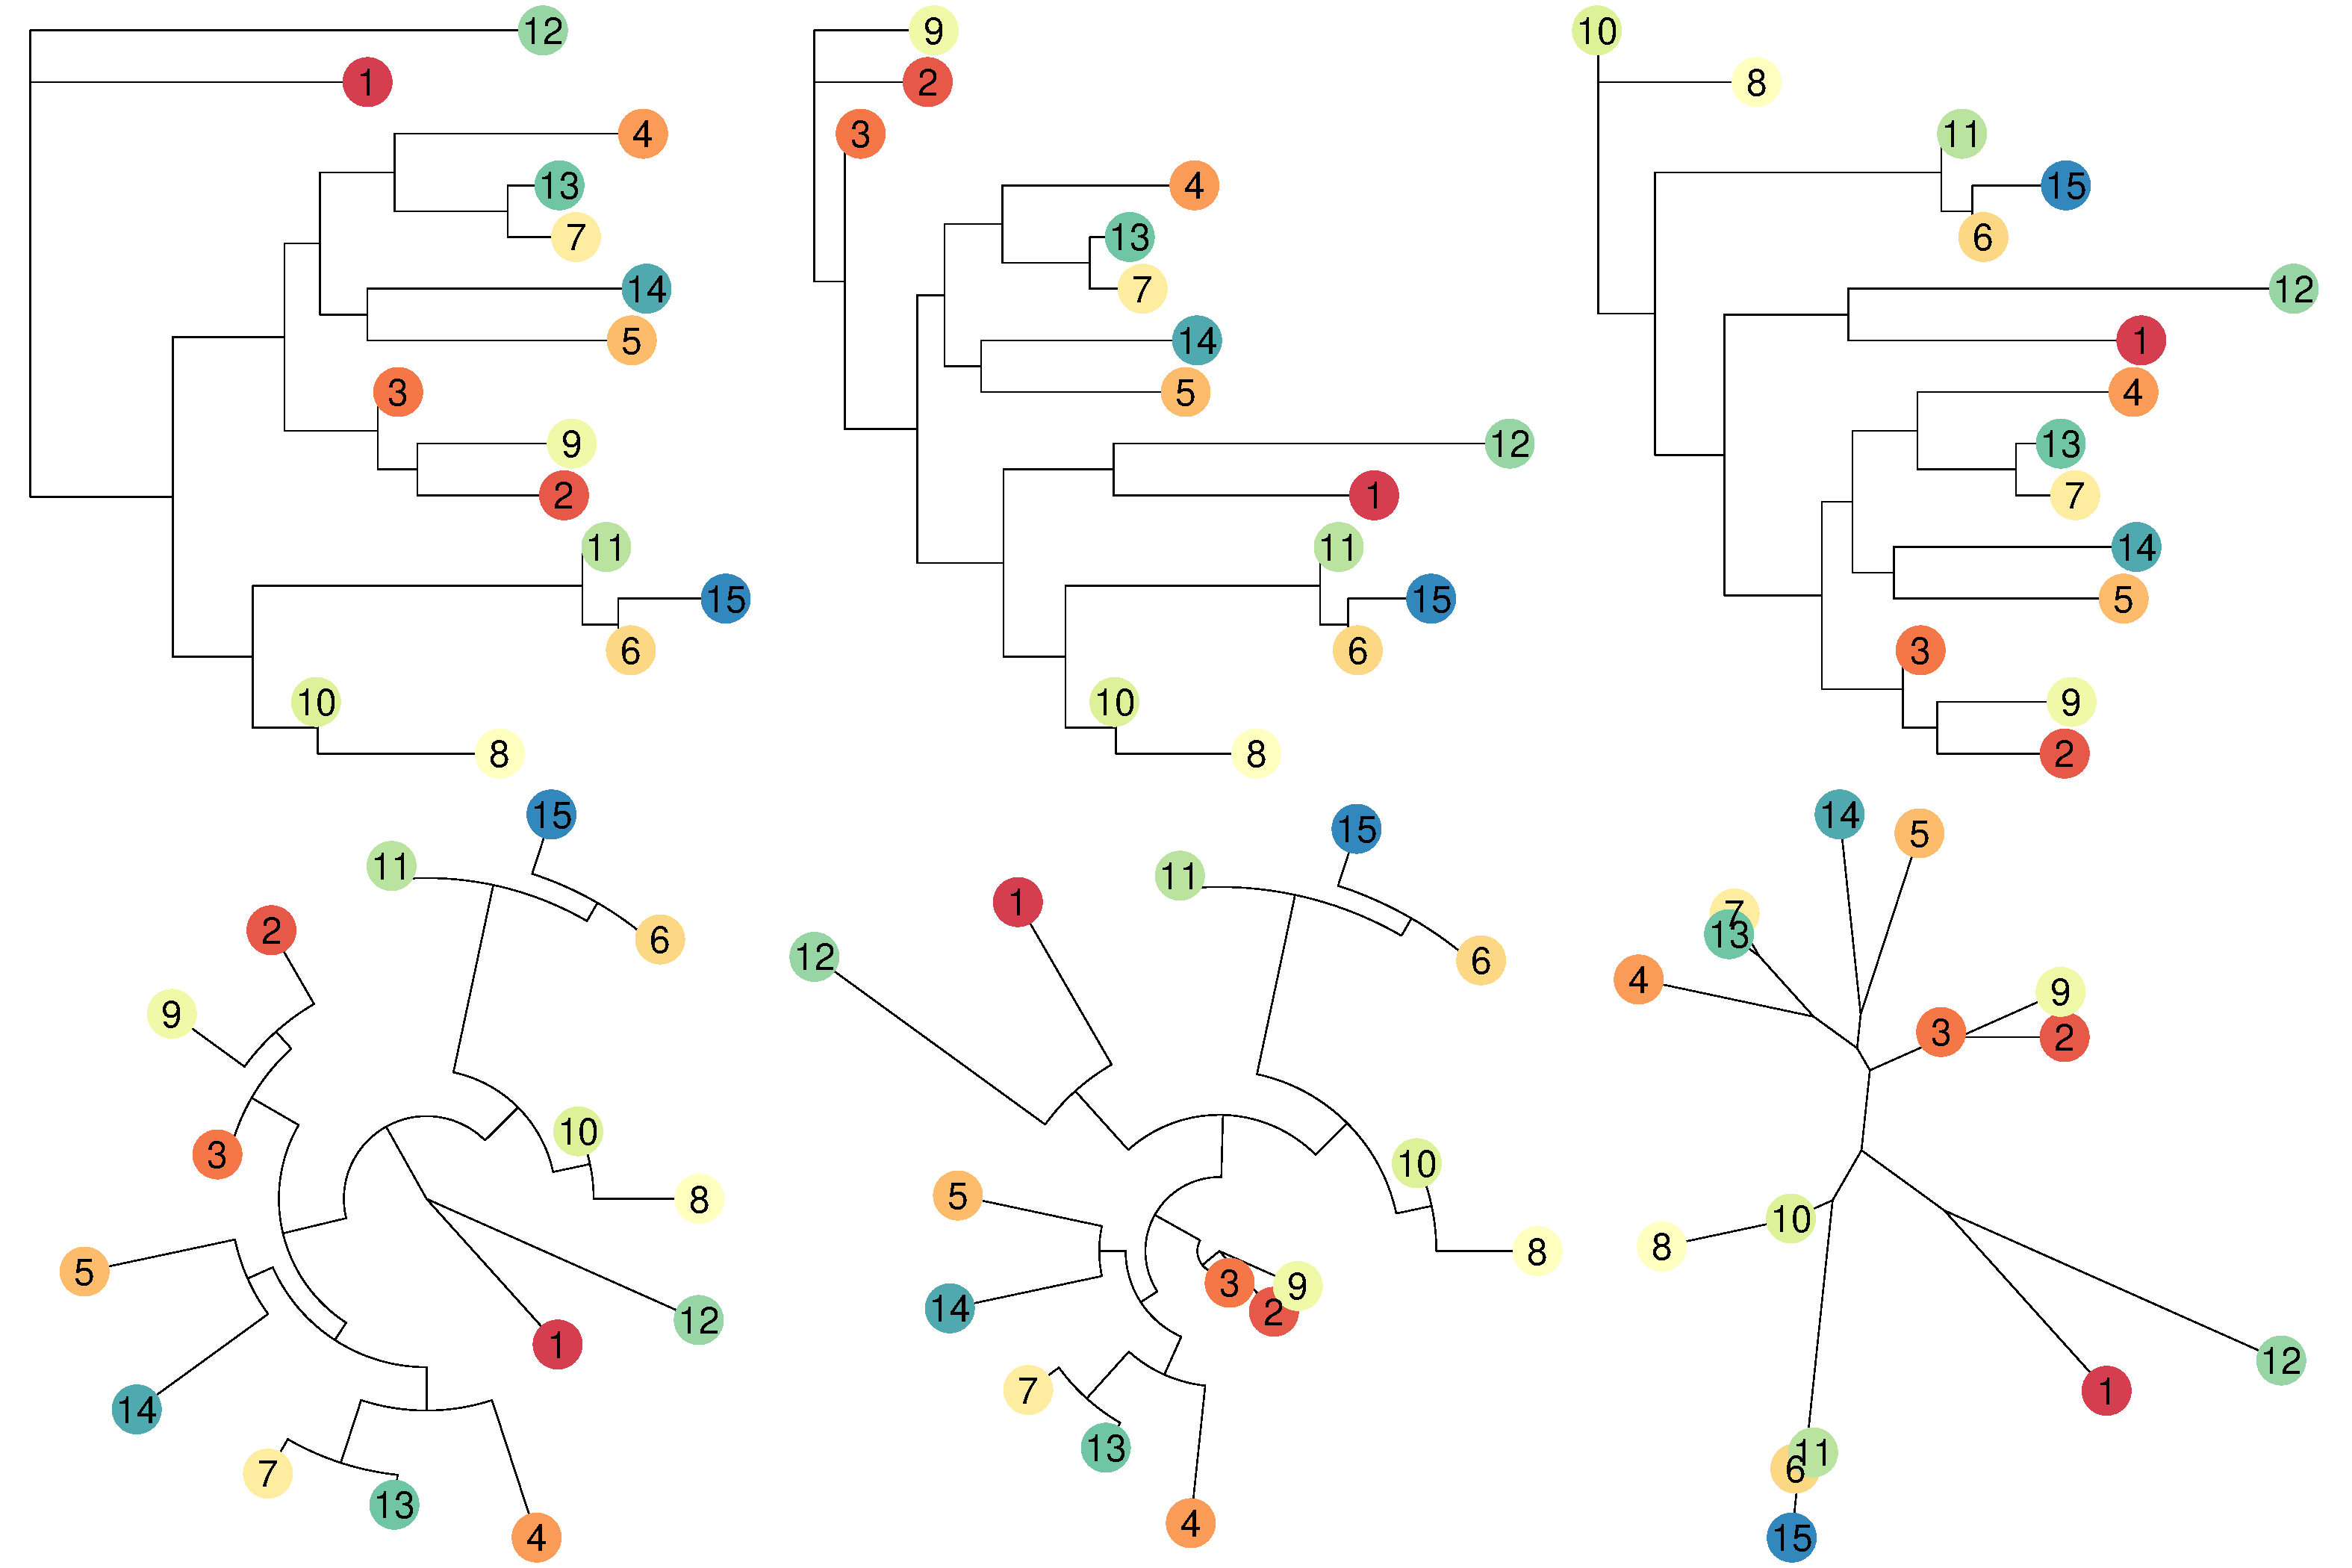
\includegraphics{figs/6trees}}}

    \pause
Never plot an unrooted tree as rooted.
\end{center}

\end{frame}
%%%%%%%%%%%%%%%%%%%%
%%%%%%%%%%%%%%%%%%%%




%%%%%%%%%%%%%%%%%%%%
%%%%%%%%%%%%%%%%%%%%
\begin{frame}
  \frametitle{Interpreting distances}

\begin{center}
    \only<1>{\resizebox{.9\textwidth}{!}{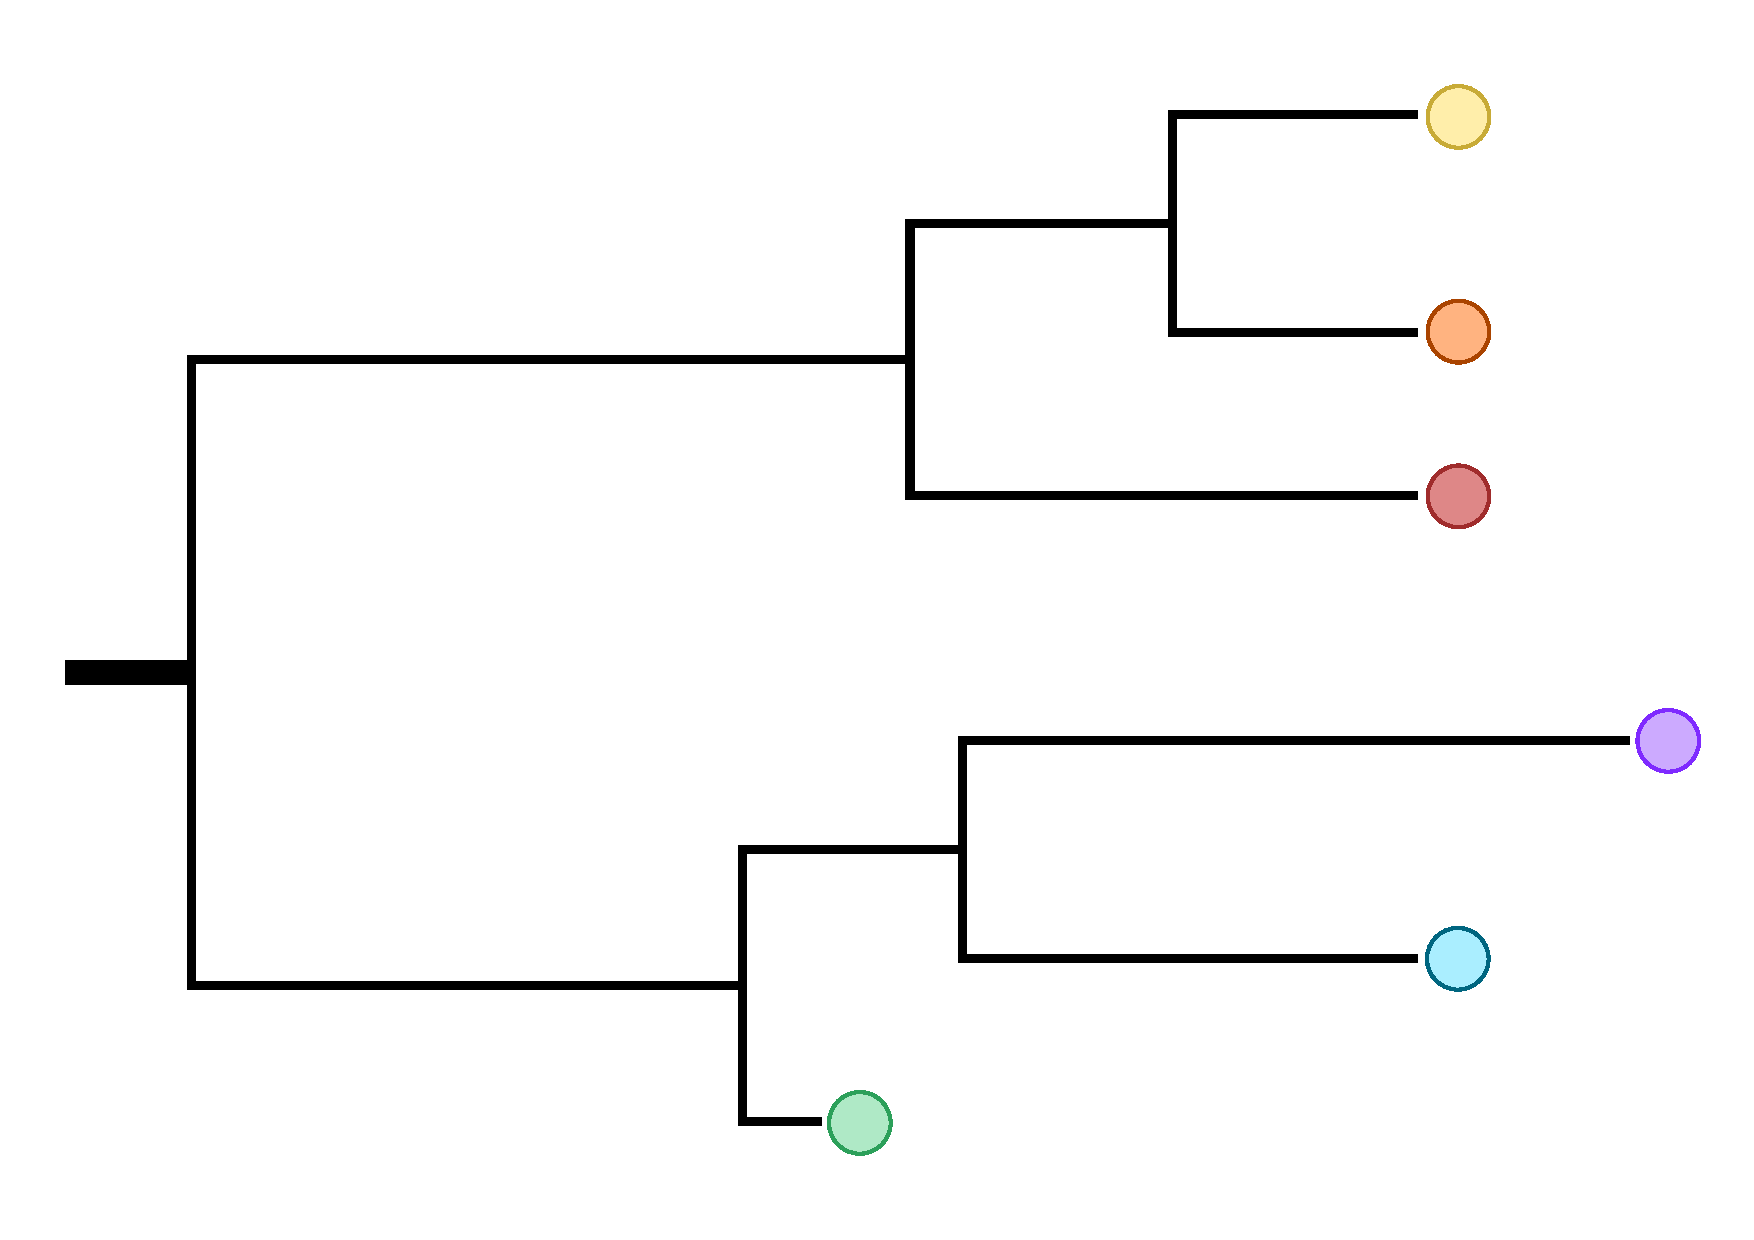
\includegraphics{figs/pitfallsLateral1}}}\only<2>{\resizebox{.9\textwidth}{!}{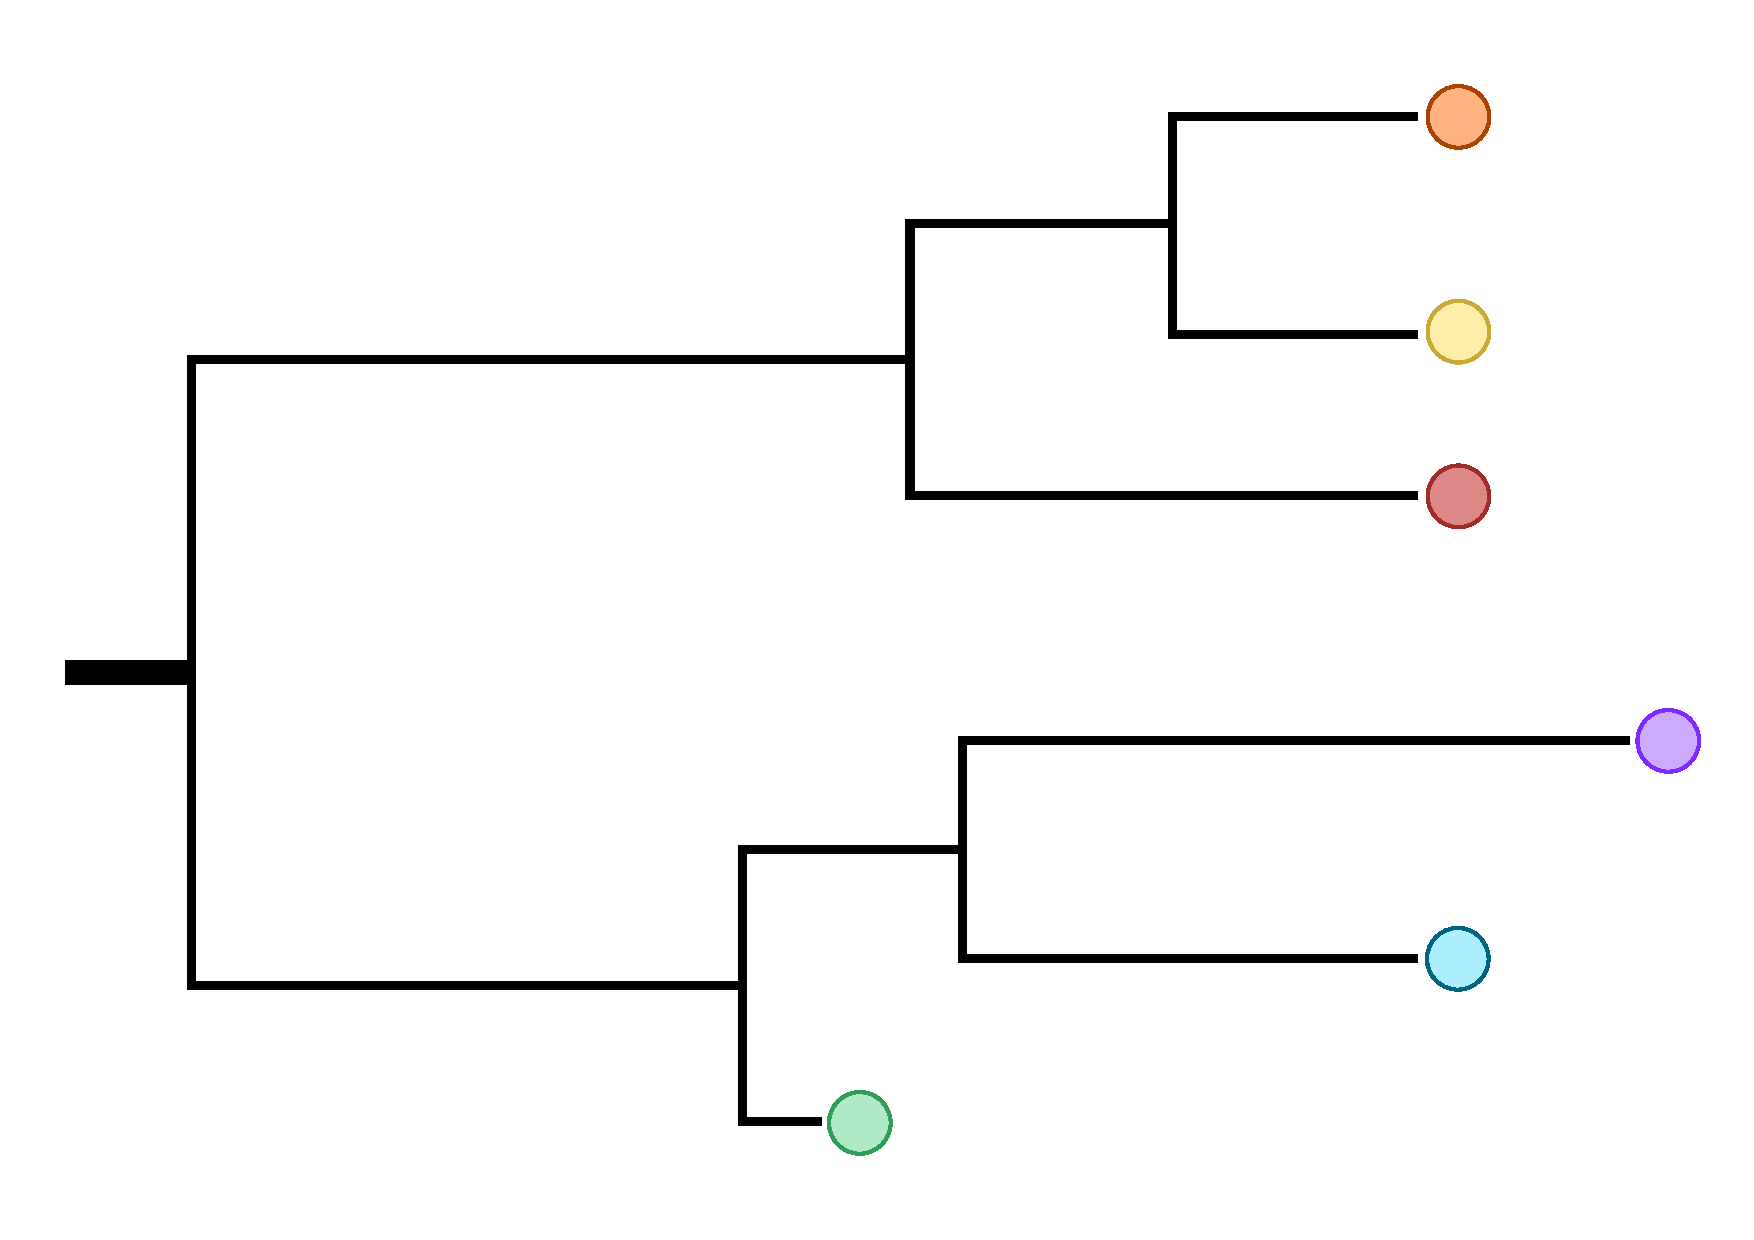
\includegraphics{figs/pitfallsLateral2}}}\only<3->{\resizebox{.9\textwidth}{!}{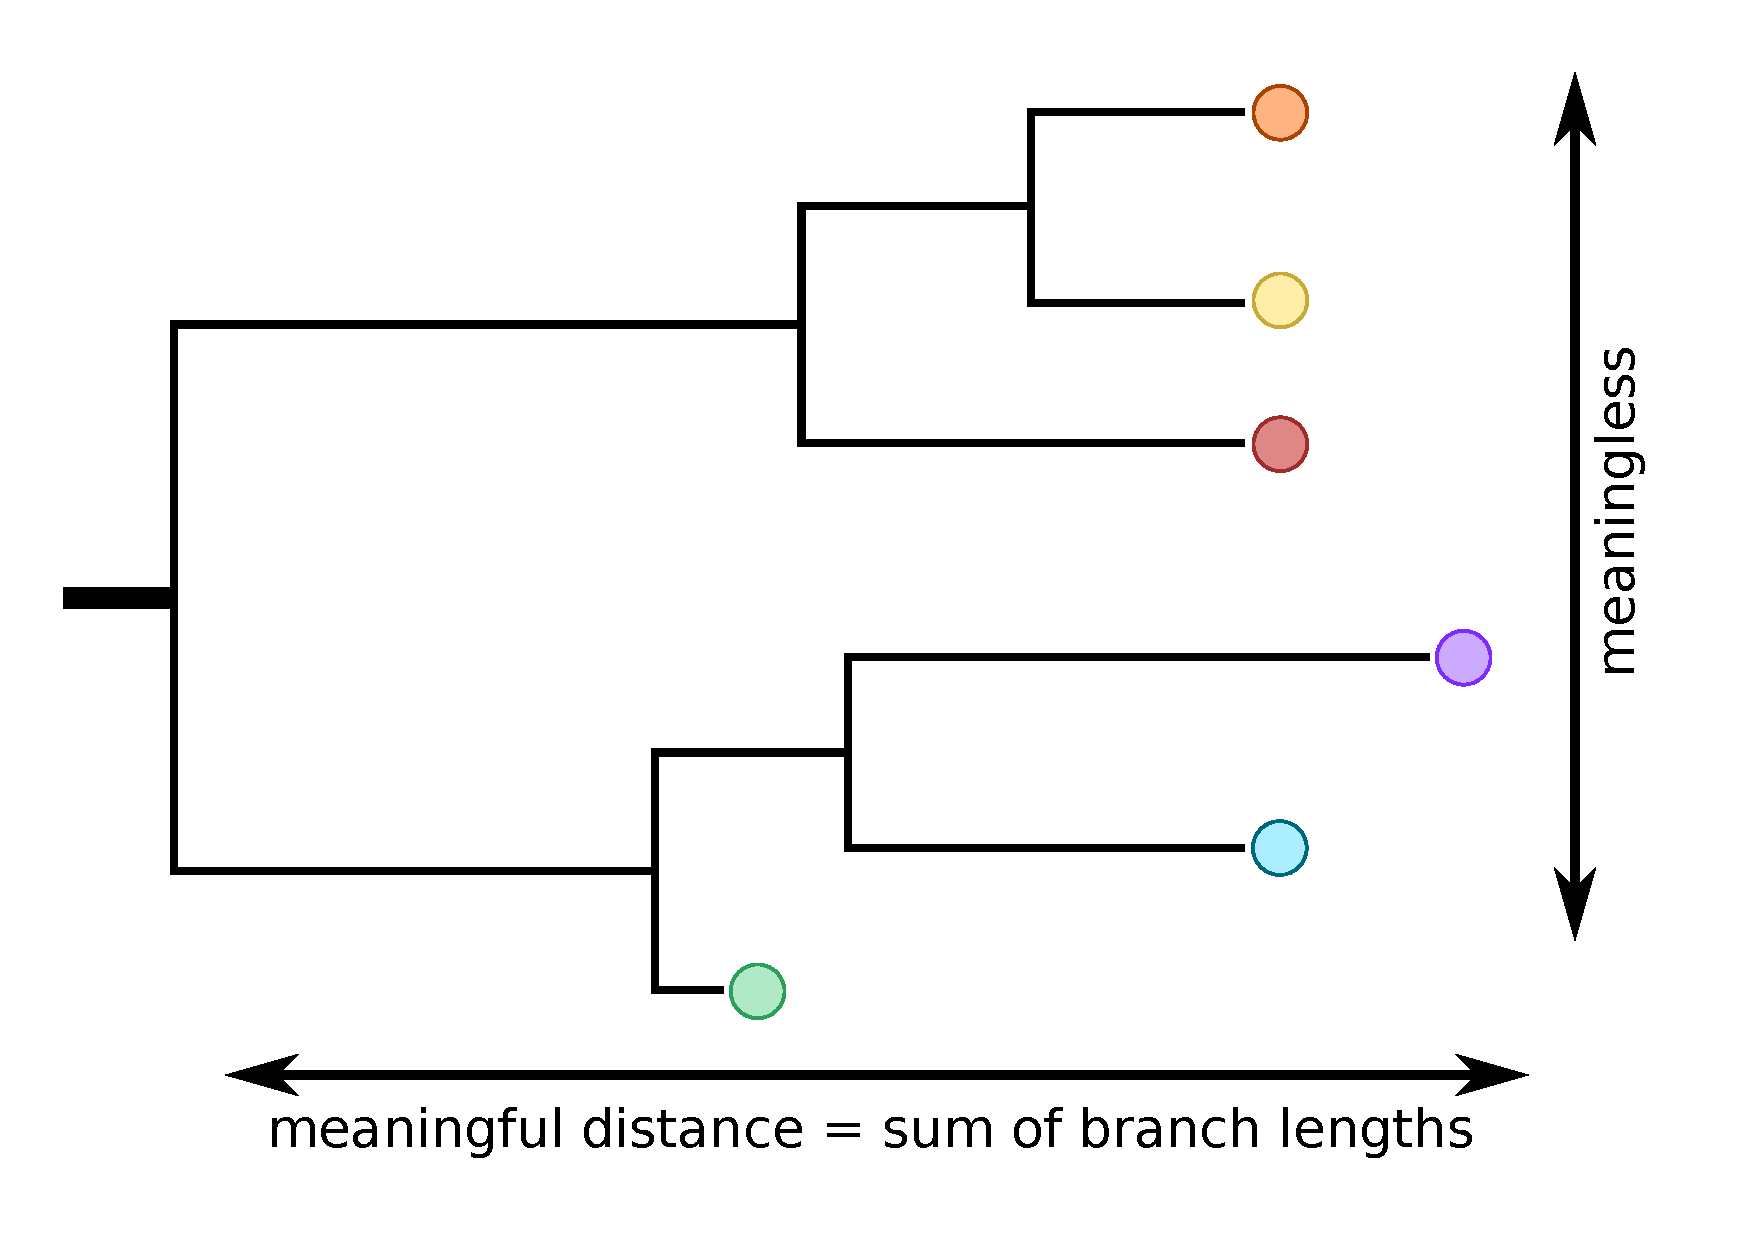
\includegraphics{figs/pitfallsLateral3}}}

% \pause
% \pause
% Only one axis makes sense.
% 
% \pause
% Distances between tips = sums of branch length
\end{center}

\end{frame}
%%%%%%%%%%%%%%%%%%%%
%%%%%%%%%%%%%%%%%%%%





%%%%%%%%%%%%%%%%%%%%
%%%%%%%%%%%%%%%%%%%%
\begin{frame}
  \frametitle{The paradox of divergent clusters}

\begin{center}
    \only<1>{\resizebox{.8\textwidth}{!}{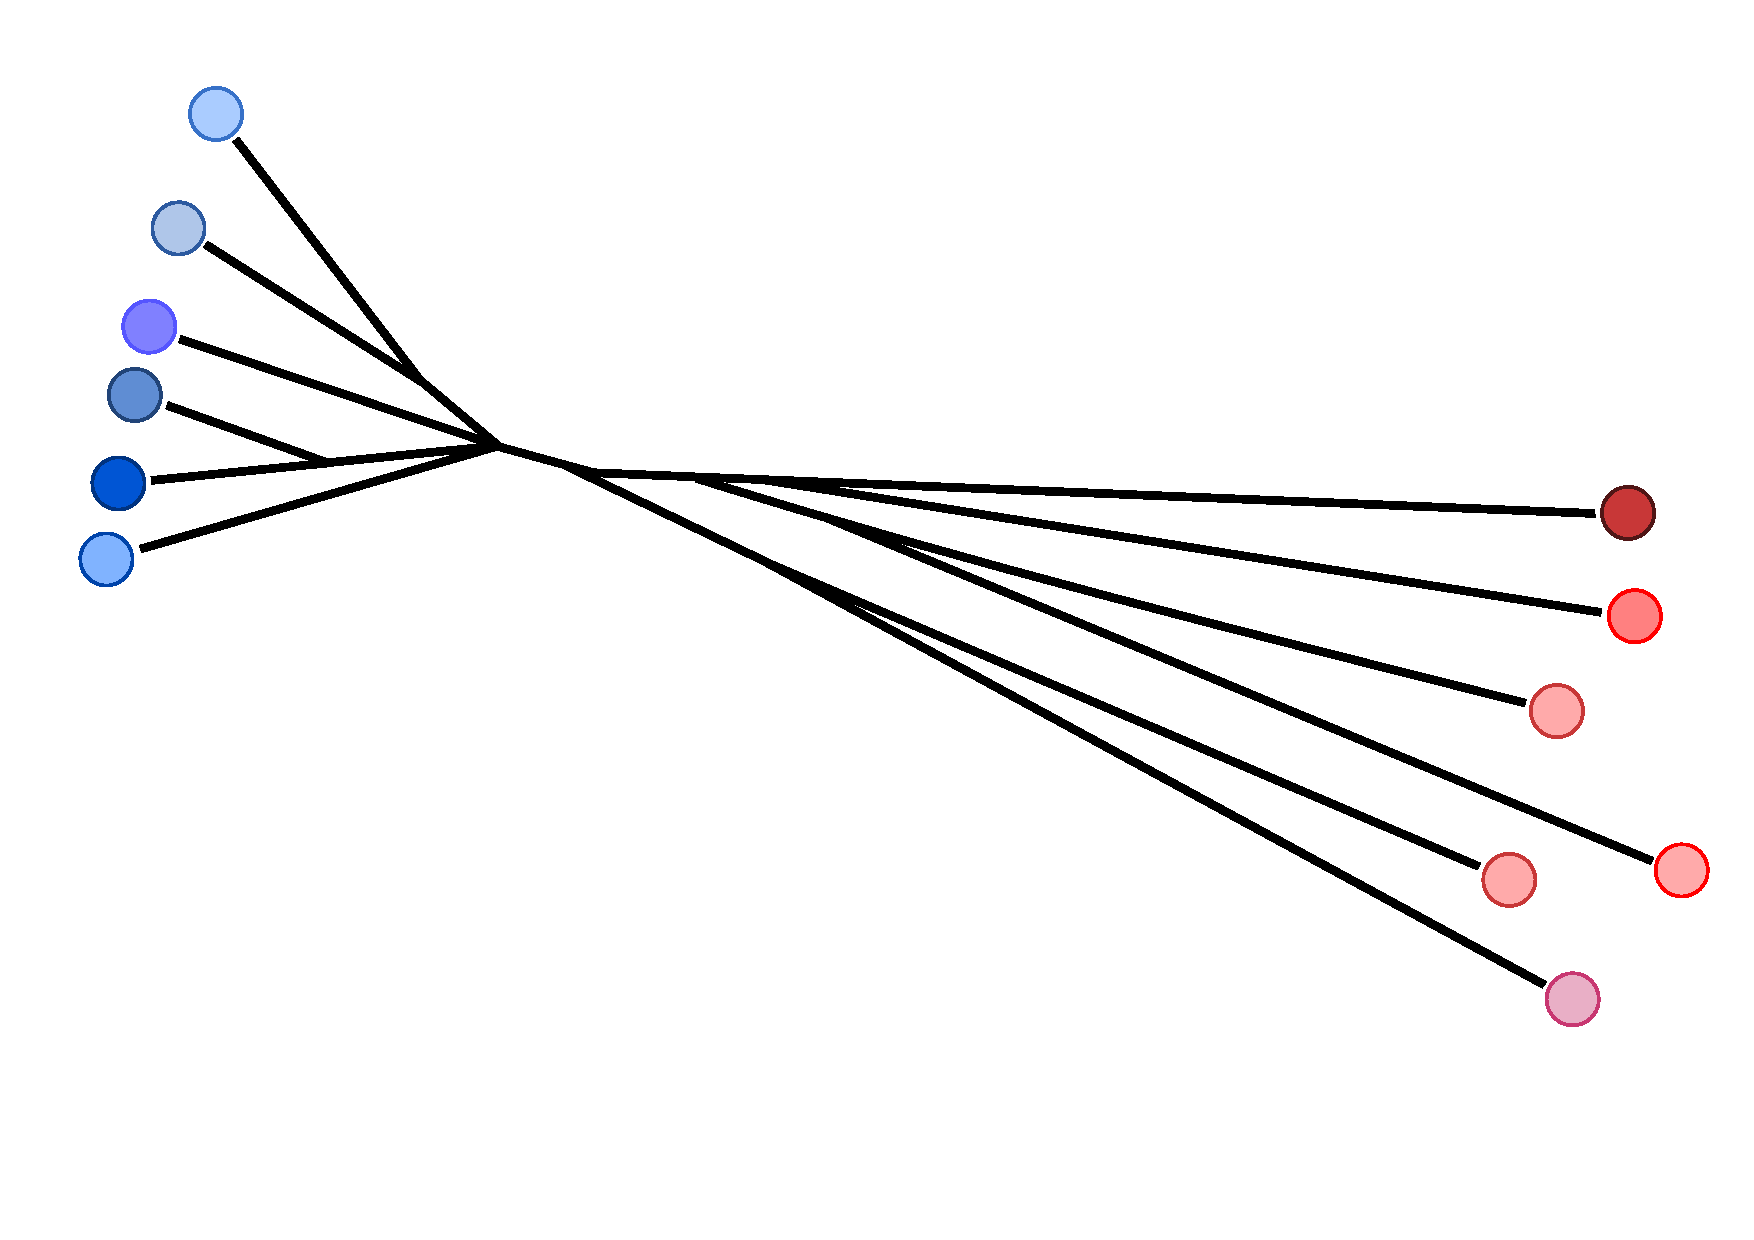
\includegraphics{figs/distanceParadox1}}}\only<2->{\resizebox{.8\textwidth}{!}{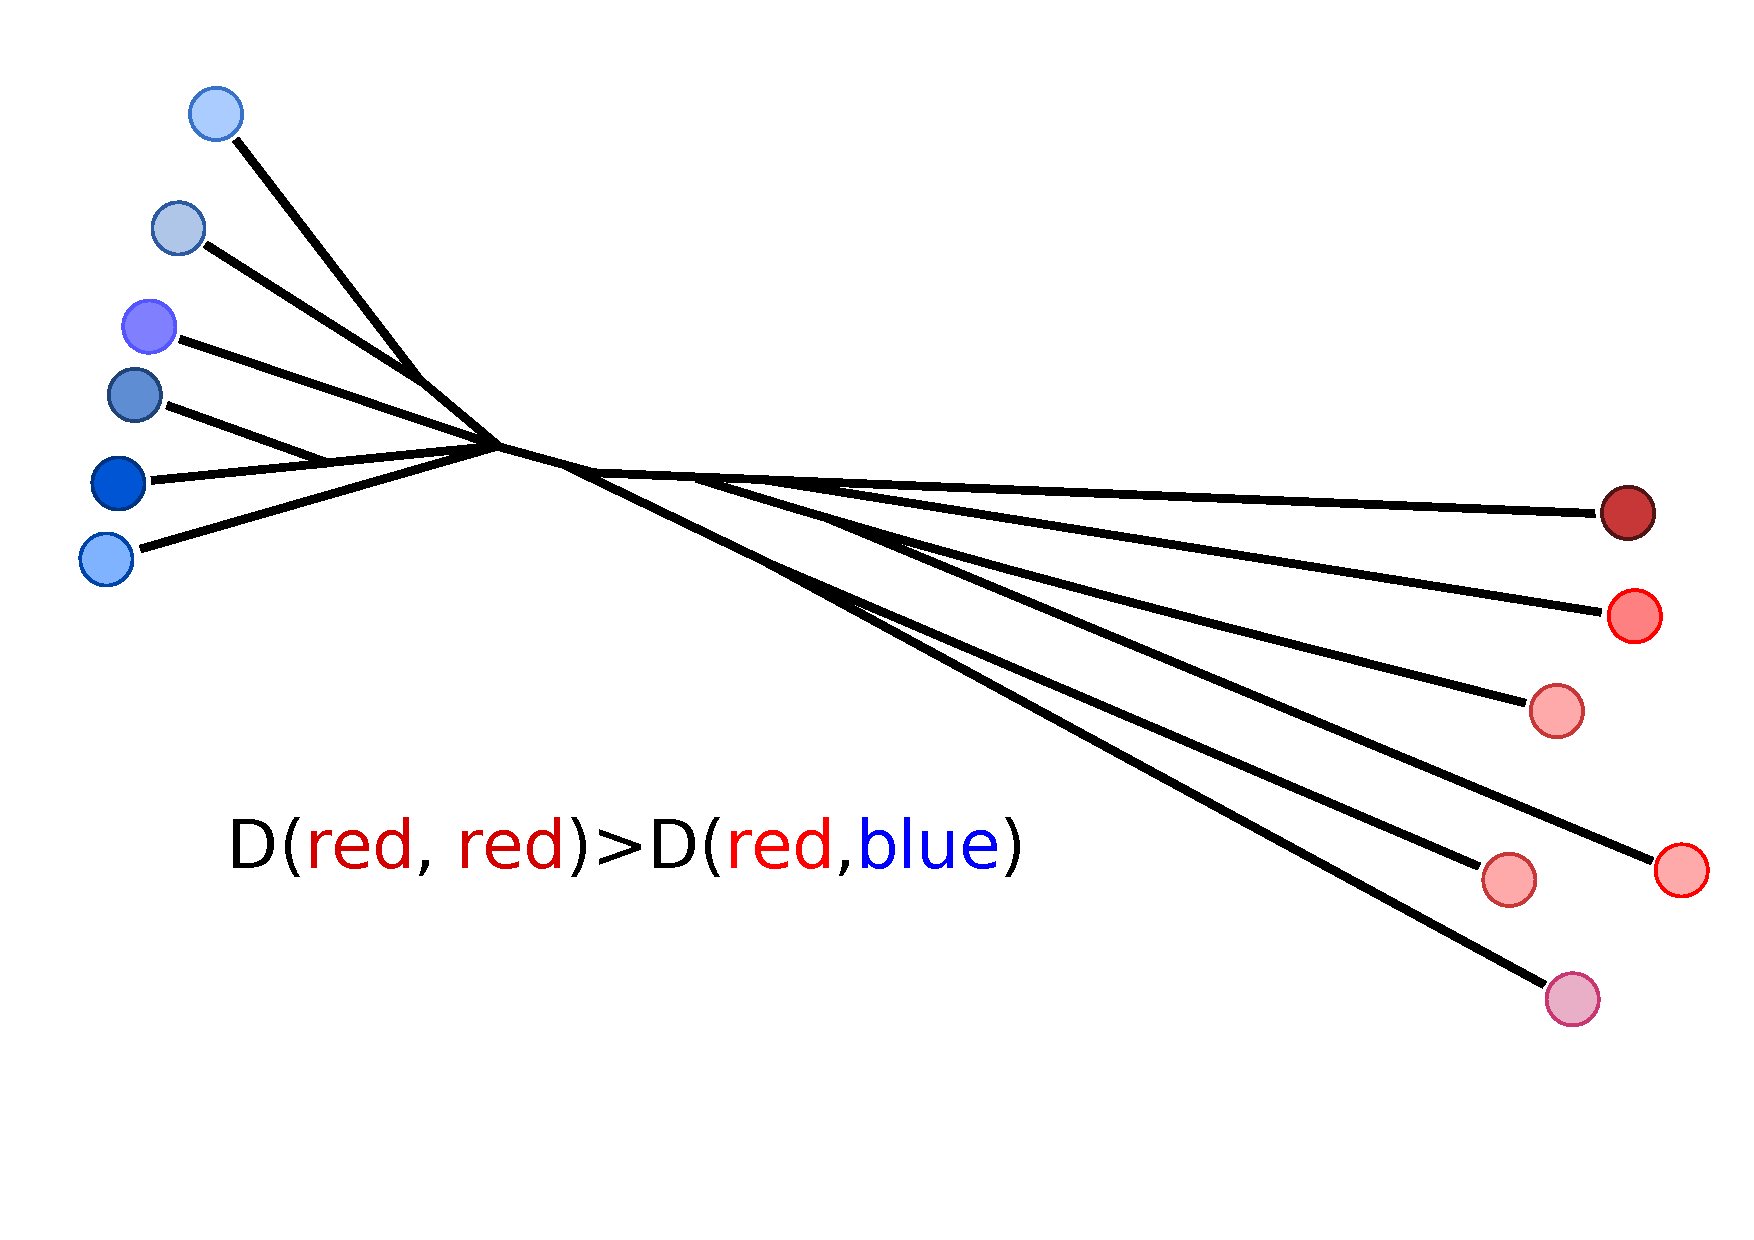
\includegraphics{figs/distanceParadox2}}}

    \pause
    \pause
MRCA and genetic distances may give different information.
\end{center}


\end{frame}
%%%%%%%%%%%%%%%%%%%%
%%%%%%%%%%%%%%%%%%%%





%%%%%%%%%%%%%%%%%%%%
%%%%%%%%%%%%%%%%%%%%
\begin{frame}
  \frametitle{Taking uncertainty into account}

\begin{center}
    \only<1>{\resizebox{\textwidth}{!}{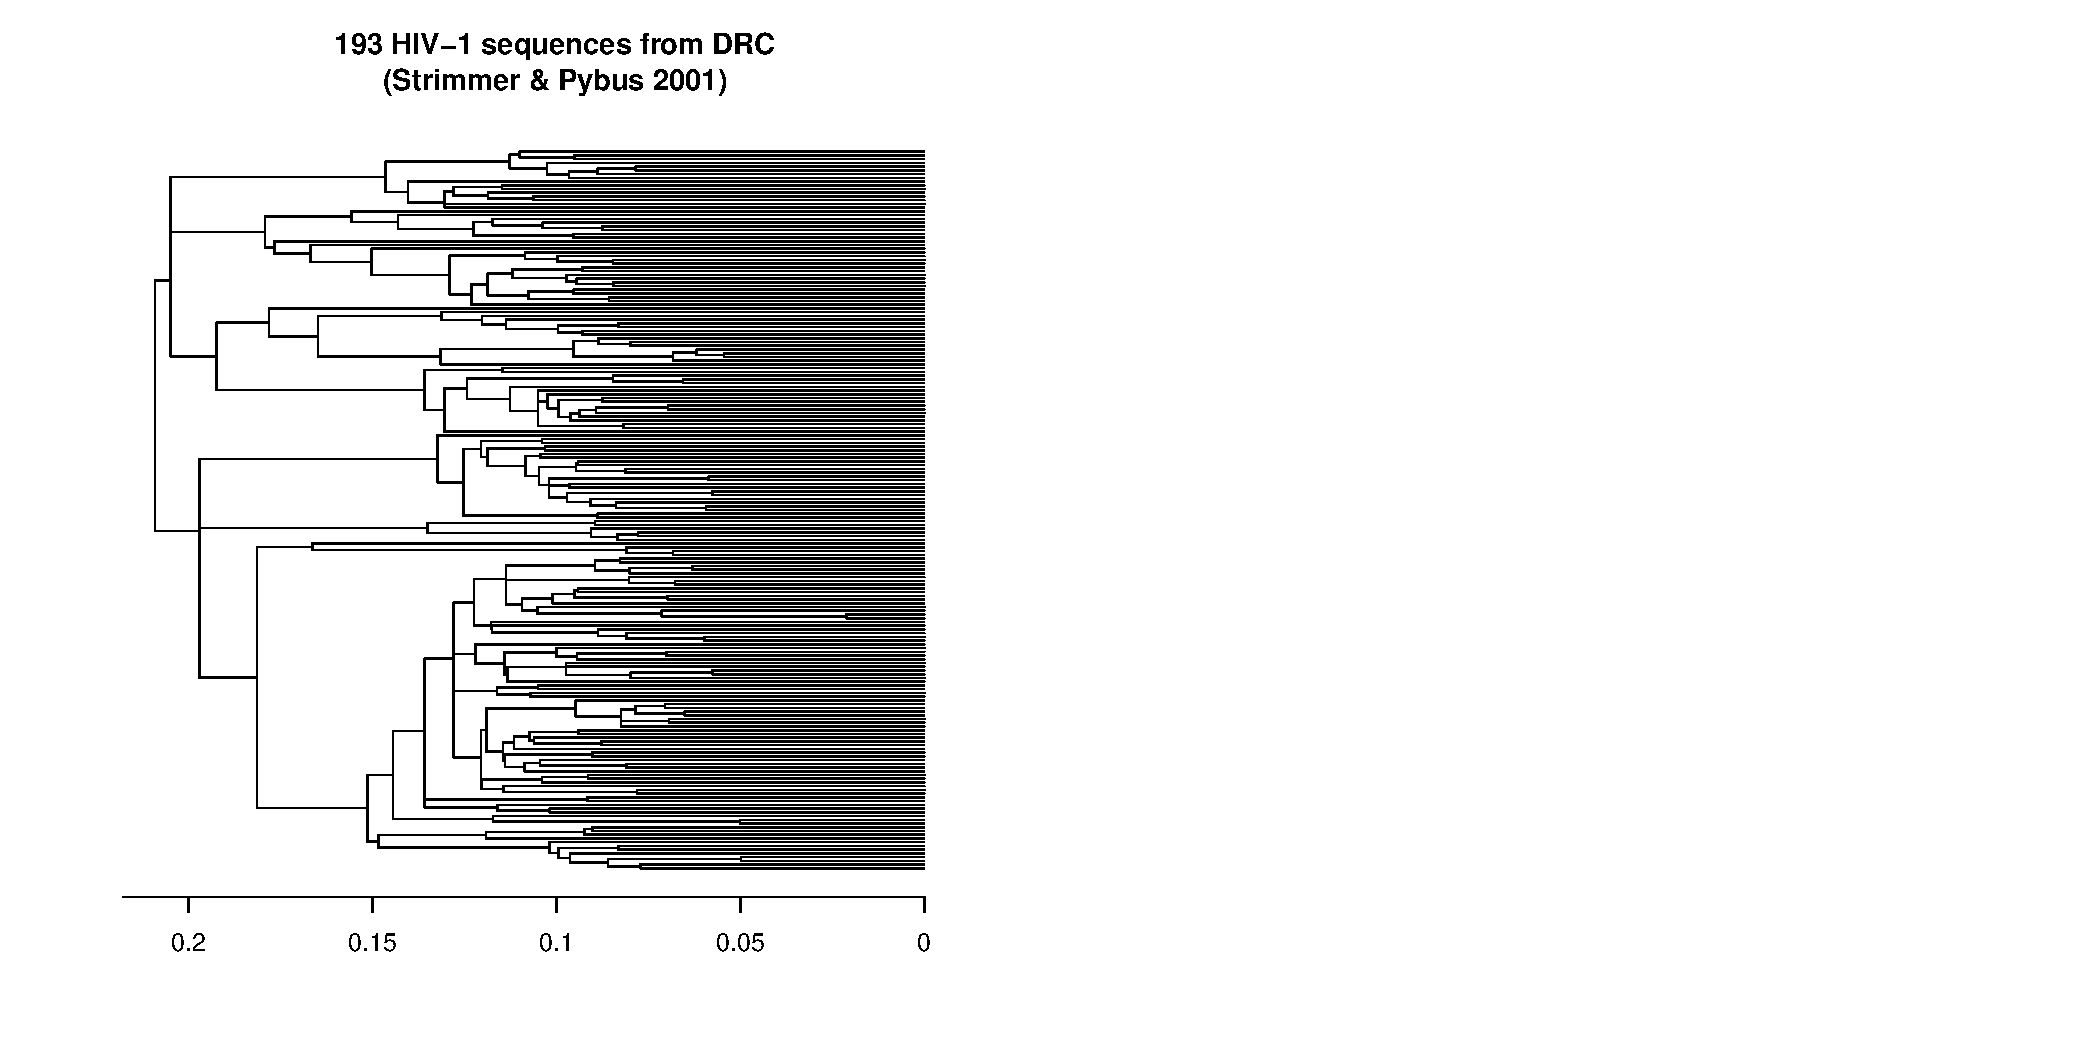
\includegraphics{figs/hivtree1}}}\only<2->{\resizebox{\textwidth}{!}{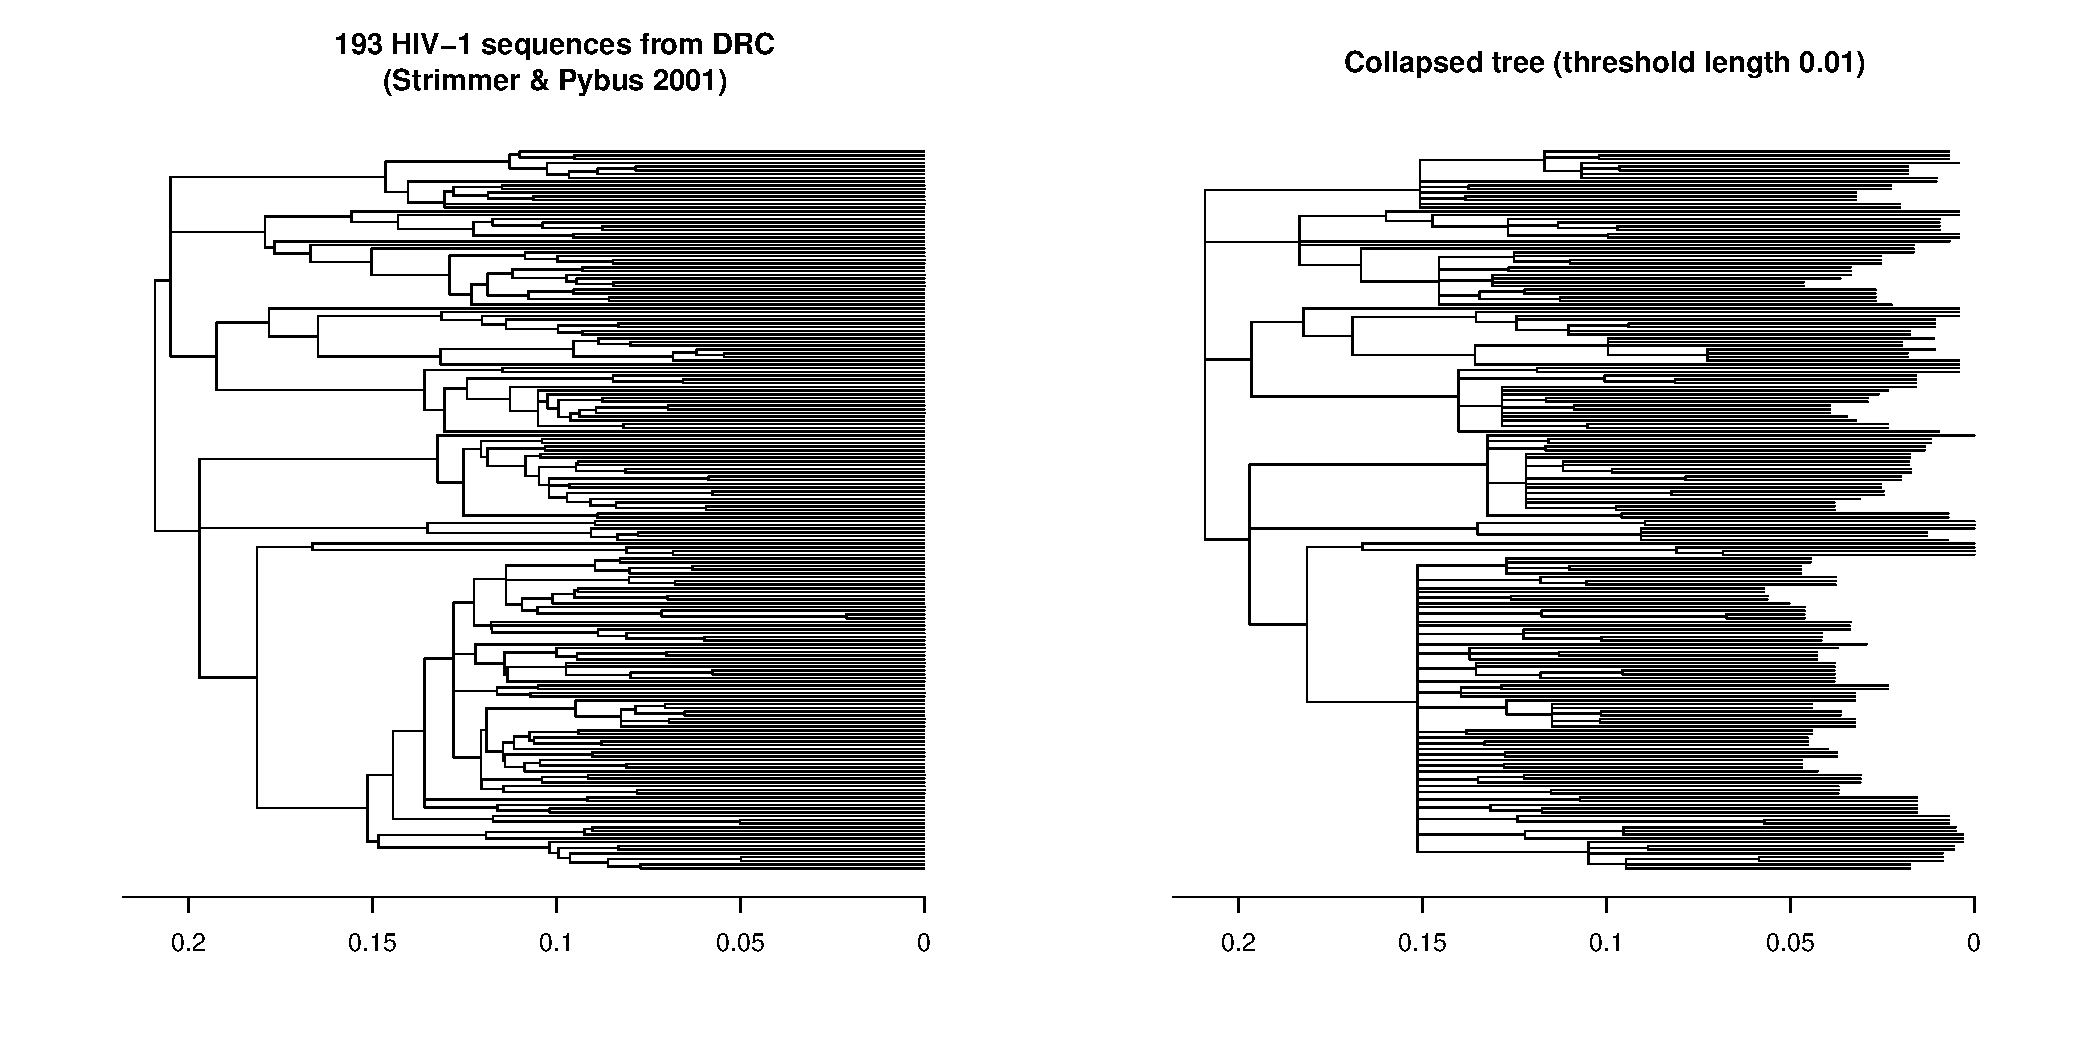
\includegraphics{figs/hivtree2}}}
    \pause
    \pause
At best, the tree is an estimate of the likely evolutionary history of the taxa studied.
\end{center}


\end{frame}
%%%%%%%%%%%%%%%%%%%%
%%%%%%%%%%%%%%%%%%%%





%%%%%%%%%%%%%%%%%%%%
%%%%%%%%%%%%%%%%%%%%
\begin{frame}
  \frametitle{(Over, Mis)Interpreting temporal trends}

\begin{center}
    \only<1>{\resizebox{\textwidth}{!}{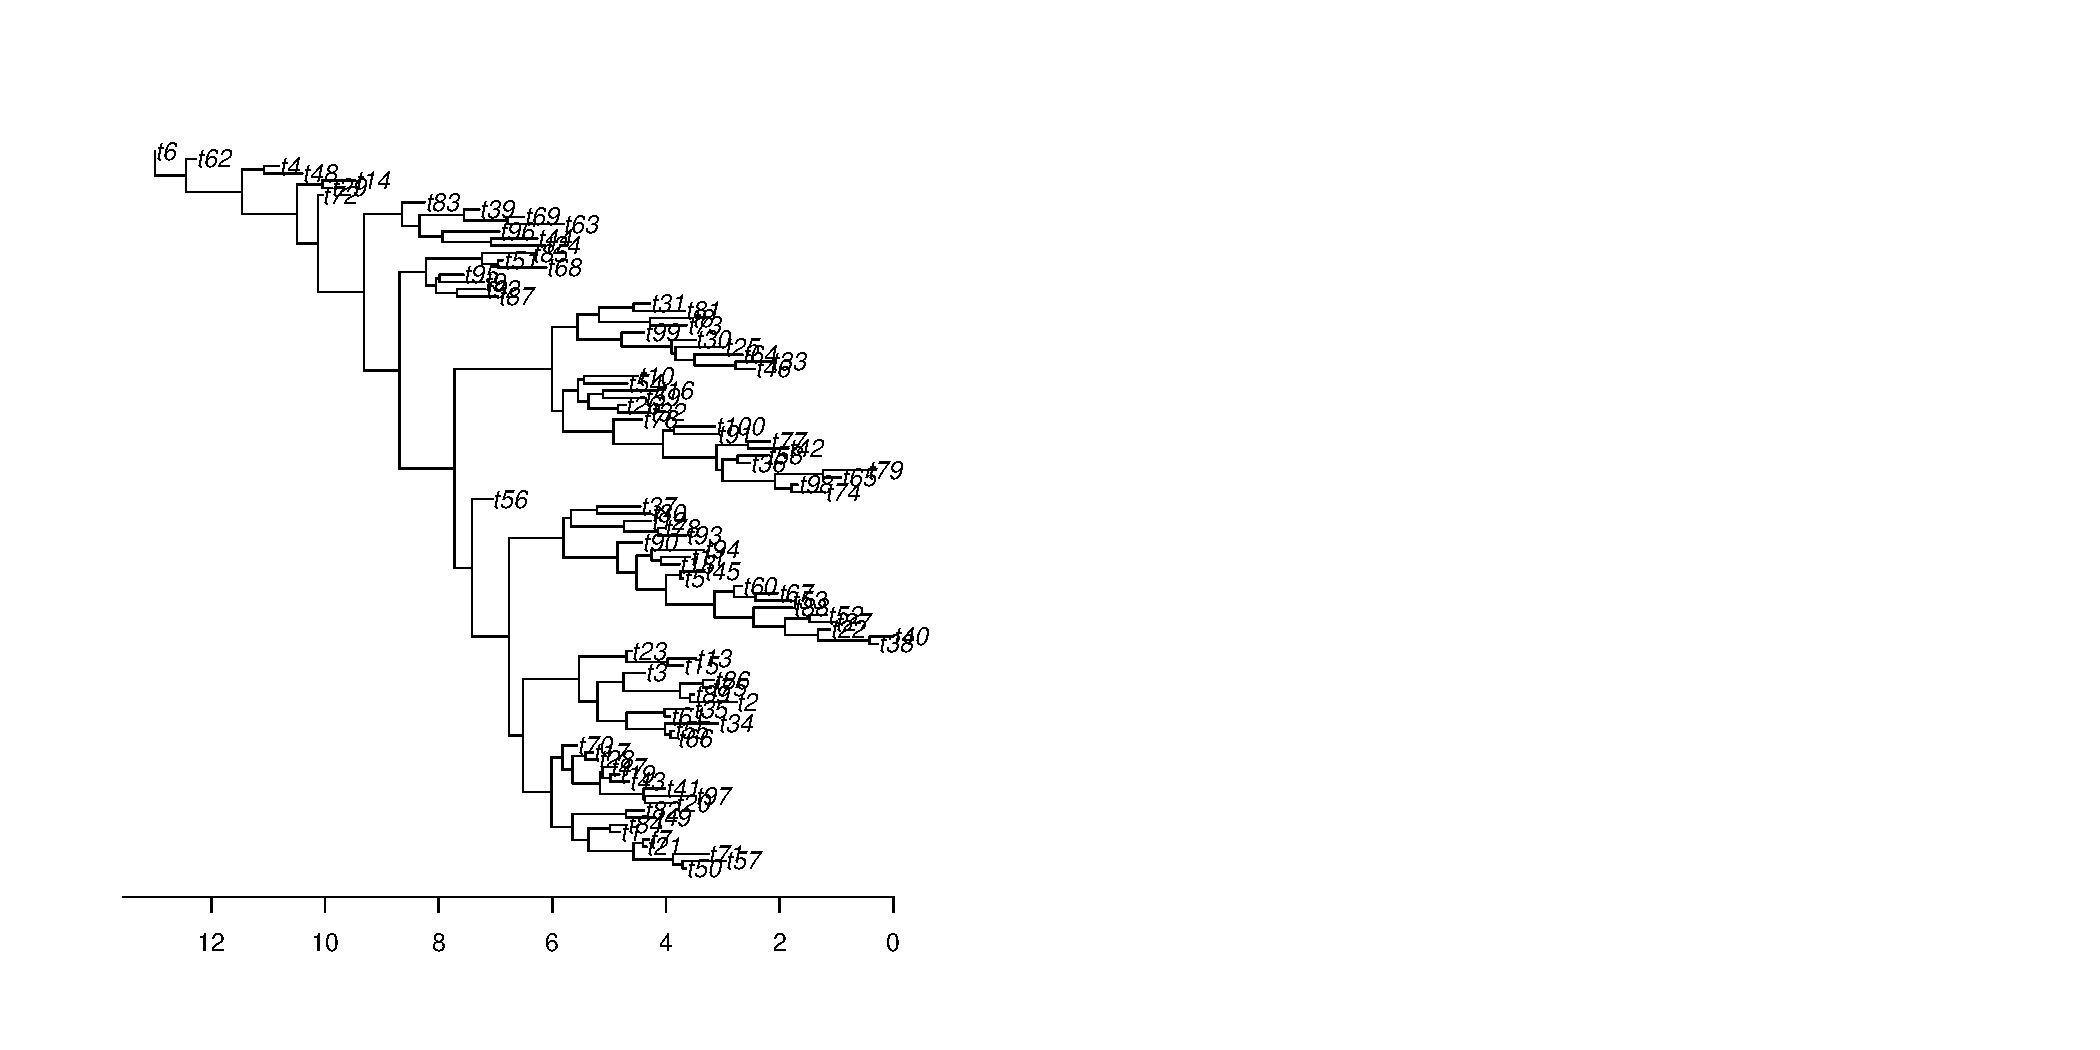
\includegraphics{figs/molecularClock1}}}\only<2->{\resizebox{\textwidth}{!}{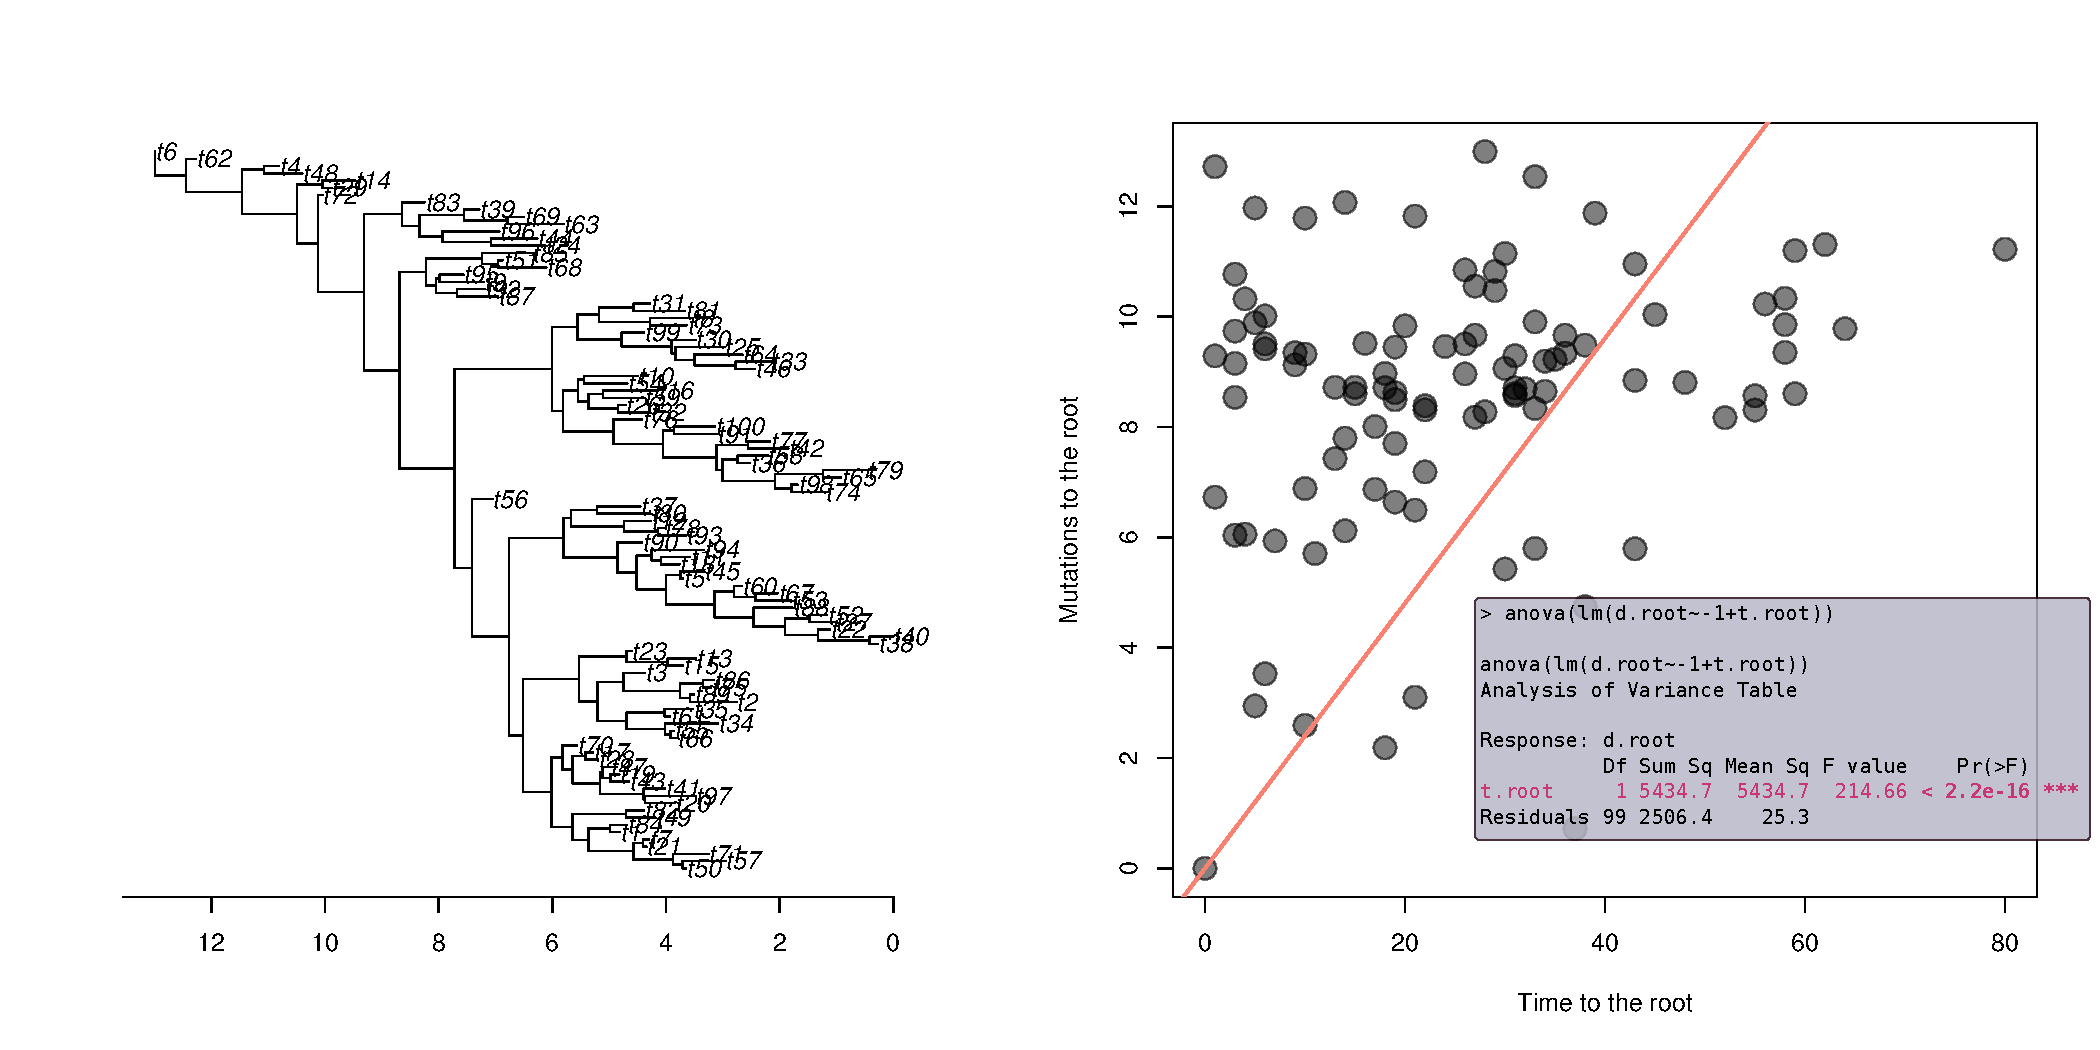
\includegraphics{figs/molecularClock2}}}

    \pause
    \pause
``Time trees'' only make sense under a near-perfect molecular clock.
\end{center}


\end{frame}
%%%%%%%%%%%%%%%%%%%%
%%%%%%%%%%%%%%%%%%%%




%%%%%%%%%%%%%%%%%%%%
%%%%%%%%%%%%%%%%%%%%
\section{And more...}
\subsection{~}
%%%%%%%%%%%%%%%%%%%%
%%%%%%%%%%%%%%%%%%%%


%%%%%%%%%%%%%%%%%%%%
%%%%%%%%%%%%%%%%%%%%
\begin{frame}
  \frametitle{This is only the beginning}

Many things can be done with trees
\begin{columns}[l]
    \column{0.6\textwidth}
\begin{itemize}
  \item estimate divergence time \pause
  \item model trait evolution (phylogenetic comparative method) \pause
  \item reconstruct ancestral states \pause
  \item measure diversity \pause
  \item infer past demographics/effective population size (coalescence) \pause
  \item ...\pause
  \item \textbf{and also, other approaches than phylogenetics to analyse genetic data}
\end{itemize}
    \column{0.4\textwidth}
           \resizebox{\textwidth}{!}{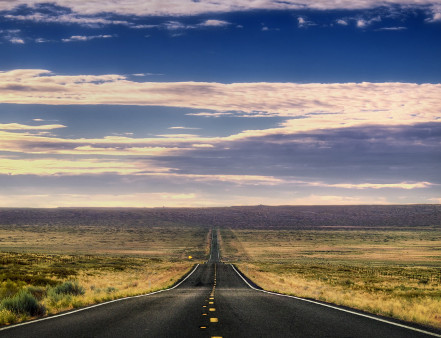
\includegraphics{figs/longroad}}
\end{columns}

\end{frame}
%%%%%%%%%%%%%%%%%%%%
%%%%%%%%%%%%%%%%%%%%




%%%%%%%%%%%%%%%%%%%%%%%%%%%%
%%%%%%%%%%%%%%%%%%%%%%%%%%%%
\begin{frame}[fragile]
  \frametitle{~}
  ~\\
  ~\\
  
  \begin{center}
    
\includegraphics[width=.7\textwidth]{figs/the-end.jpg}
  \end{center}

\end{frame}
%%%%%%%%%%%%%%%%%%%%%%%%%%%%
%%%%%%%%%%%%%%%%%%%%%%%%%%%%




\end{document}




% %%%%%%%%%%%%%%%%%%%%
% %%%%%%%%%%%%%%%%%%%%
% \begin{frame}
%   \frametitle{Frame title}
% 
% \begin{block}{Title}
% \begin{itemize}
%   \item 
%   \item 
% \end{itemize}
% \end{block}
% 
% \end{frame}



